\documentclass[a4paper, 10pt, titlepage]{article}
% PACKAGES
\pdfpagewidth
\paperwidth
\pdfpageheight
\paperheight
\usepackage[english,italian]{babel} 
\usepackage{epsfig}
\usepackage{fancyhdr} 
\usepackage{amsmath,amssymb}
\usepackage{amscd}
\usepackage{amsthm} % per i teoremi
\usepackage[T1]{fontenc} 
\usepackage[utf8]{inputenc} 
\usepackage[usenames,dvipsnames]{xcolor}
\usepackage{graphicx}
\usepackage{hologo}
\usepackage[document]{ragged2e}
\frenchspacing 
\usepackage{geometry}
\geometry{a4paper,tmargin=2cm,bmargin=2cm, lmargin=2.8cm,rmargin=2.8cm} 
\usepackage{booktabs}
\usepackage{longtable}
\usepackage{colortbl}
\usepackage{multirow}
\usepackage{float}
\usepackage{svg}
\usepackage[caption=true,font={tt,bf,sc},listofformat=subsimple, labelformat=empty]{subfig}
\usepackage{hyperref}
\hypersetup{
  colorlinks   = true,    % Colours links instead of ugly boxes
  urlcolor     = blue,    % Colour for external hyperlinks
  linkcolor    = black,    % Colour of internal links
  citecolor    = blue      % Colour of citations
}
\usepackage{natbib}
%%%%%%%%%%%%%%%%%%%%%%%%%%%%%%%%%%%%%%%%%%%%%%%%%%%%%%%%%%%%%%%%%%%%%%%%%%%%%%
\definecolor{MyGreen}{HTML}{ccff99}
\definecolor{MyGold}{HTML}{ffe066}
\definecolor{MyOrange}{HTML}{ffc266}
\newcommand{\clrmatch}[0]{MyGold}
\newcommand{\clrpath}[0]{MyOrange}
\newcommand{\clrnew}[0]{blue}
%%%%%%%%%%%%%%%%%%%%%%%%%%%%%%%%%%%%%%%%%%%%%%%%%%%%%%%%%%%%%%%%%%%%%%%%%%%%%%
%INTERLINEA
\linespread{1.2}
\newcommand\frontmatter{%
    %\cleardoublepage
  %\@mainmatterfalse
  \pagenumbering{roman}}

\newcommand\mainmatter{%
    %\cleardoublepage
 % \@mainmattertrue
  \pagenumbering{arabic}}

\newcommand\backmatter{%
  % \if@openright
  %   \cleardoublepage
  % \else
  %   \clearpage
  % \fi
 % \@mainmatterfalse
   }
% defining the \BibTeX command - from Oren Patashnik's original BibTeX documentation.
\def\BibTeX{{\rm B\kern-.05em{\sc i\kern-.025em b}\kern-.08emT\kern-.1667em\lower.7ex\hbox{E}\kern-.125emX}}
\begin{document}
    \begin{titlepage}
        \begin{center}
            
\includegraphics [width=.15\columnwidth, angle=0]{unisa}\\ % height
            \vspace{0.5cm}
            {\LARGE \scshape Università degli Studi di Salerno}\\
            \vspace{0.5cm}
            {\Large Dipartimento di Informatica}\\
            \vspace{0.1cm}
            {\large Strumenti Formali per la Bioinformatica}\\
            \vspace{1.5cm}
            {\Large \scshape Relazione di Progetto} \\
            \vspace{4cm}
            {\huge \bfseries Un approccio deep learning per la classificazione delle varie tipologie di forme tumorali tramite uso delle espressioni genetiche, individuando potenziali biomarker} \\ 
            \vspace{2cm}
        \end{center}   
        \begin{minipage}[t]{6cm}
        \flushleft
        \textsc{Docenti:}\\
        Prof.ssa \textbf{Clelia De Felice} \\
        Prof.ssa \textbf{Rosalba Zizza} \\
        Prof. \textbf{Rocco Zaccagnino} \\
        %{\small Università degli studi di Salerno} \\[0.25cm]
        \end{minipage}
        \hfill
        \begin{minipage}[t]{6cm}
        \flushright
        \textsc{Studenti:}\\
        \textbf{Nicola Pagliara} 0522501413 \\
        {\small \url{n.pagliara1@studenti.unisa.it}} \\
        \textbf{Gaetano Antonucci} 0522500941\\
        {\small \url{g.antonucci2@studenti.unisa.it}} \\
        \end{minipage}
        \vspace{3cm}
        \begin{center}
            {\small Anno Accademico 2022-2023} 
        \end{center}   
    \end{titlepage}
    % ABSTRACT
    \pagenumbering{gobble}
    \frontmatter
    % TESTO GIUSTIFICATO
    \justifying
    % ABSTRACT
    \renewcommand{\abstractname}{Abstract}
    \begin{abstract}
L'analisi differenziale è la parte più significativa dell'analisi delle RNA-Seq. 
I metodi convenzionali di solito mettono in corrispondenza i sample tumorali con
i sample normali provenienti dalla stessa tipologia di tumore. Tali metodi, però,
potrebbero fallire nel differenziare i diversi tipi di timore siccome non possono
sfruttare la conoscenza proveniente da altre tipologie di tumore. Il Pan-Cancer
Atlas fornisce informazioni molto ampie sulle 33 classi prevalenti di tumori che
possono essere utilizzate come conoscenza base per generare biomarker specifici
a seconda della classe tumorale. In questo lavoro abbiamo dapprima replicato
il lavoro svolto nel paper \cite{lyu2018deep} inglobando i dati ad alta dimensionalità
delle RNA-Seq in immagini 2D al fine di usare una rete neurale convoluzionale
(CNN) per eseguire la classificazione delle 33 classi tumorali. 
L'accuracy finale ottenuta è stata del $94.74\%$. 
Abbiamo poi provato, come variante a quanto svolto in \cite{lyu2018deep}, a
modificare i parametri di addestramento della CNN al fine di migliorarne le
performance ma abbiamo ottenuto un'accuracy complessiva del $94.83\%$ che è inferiore
a quanto ottenuto da \cite{lyu2018deep}. Tuttavia abbiamo ottenuto dei miglioramenti
per singola coorte tumorale, come ad esempio ESCA, LGG e LUAD.
In seguito, seguendo quanto fatto, abbiamo sfruttato anche noi l'idea di 
Guided Grad-CAM \cite{selvaraju2017grad} e abbiamo generato, per ogni classe,
le heatmap significative per tutti i geni.
Tramite Pathway Enrichment Analysis, sui geni che hanno mostrato un'alta 
intesità nelle heatmap, è stato possibile validare che tali geni sono correlati
a specifiche path tumorali dimostrando che è possibile utilizzare tale lavoro
per la ricerca di potenziali biomarker.
\end{abstract}

% abbiamo riportato i risultati dell'accuracy GPU

    % INDICE
    \pagestyle{plain}
    \tableofcontents
    \clearpage
    % ELENCO DELLE FIGURE
    \addcontentsline{toc}{section}{Elenco delle figure}
    \listoffigures
    \clearpage
    % ELENCO DELLE TABELLE
    \addcontentsline{toc}{section}{Elenco delle tabelle}
    \listoftables
    \clearpage
    \mainmatter
    % SEZIONI
    % 1
    \section{Introduzione}
\label{sec:intro}
Grazie al miglioramento delle tecniche di sequenziamento con l'avvento dei Next Generation Sequencing methods, 
si è avuto un progressivo miglioramento in accuratezza ed efficienza anche per quanto riguarda l'analisi del genoma
umano. Un problema sempre presente anche ai giorni nostri è quello di comprendere in maniera completa e approfondita
le cause dei vari tumori. A tal fine, The Cancer Genome Atlas, si è occupato del sequenziamento e della gestione di
un grande volume di tessuti tumorali e, inoltre, ha analizzato oltre 11.000 tumori appartenenti alle 33 forme più diffuse
di cancro. A partire da tali analisi è stata incentivata la creazione del Pan-Cancer Atlas, il quale, come riportato
nella loro home page "fornisce una comprensione unica, completa, approfondita e interconnessa di come, dove e 
perché nascono i tumori nell'uomo". Il Pan-Cancer Atlas è di fatto una risorsa essenziale per lo sviluppo di nuovi
trattamenti nella ricerca della medicina personalizzata, in quanto, per ogni sample tumorale, è possibile accedere ai
suoi \textit{RNA-Seq expression data}. Tali dati sono un vantaggio quando si cerca di identificare i potenziali
biomarker per ogni tipo di tumore.

Finora, per tentare di scoprire i potenziali biomarker, molte analisi cercavano di trovare i geni che si sono espressi 
differentemente. Tali analisi, però, non tengono conto dell'espressione dei geni in altri tipi di tumore e solo legate
al tipo di tumore e/o ai dati specifici che si stanno analizzando correntemente. Di fatti, molti modelli vanno a 
simulare l'espressione dei geni ma falliscono miseramente quando si usa il modello su altri dati o su altri
tipi di tumore. Da tali fallimenti è dunque nata l'esigenza di progettare un metodo che possa includere nelle analisi
la conoscenza proveniente da più classi tumorali.

Da un altro punto di vista, la classificazione dei tumori usando i dati genomici può contribuire ad una diagnosi più
veloce e più accurata ma, di fatti, raramente viene usata in quanto è difficile lavorare con dataset genomici ad alta
dimensionalità. 
Per rendere più chiaro questo punto, basti pensare che nel Pan-Cancer Atlas gli \textit{mRNA-Seq gene expression} 
data contengono informazioni a partire da oltre 20 mila geni, molti dei quali non sono coinvolti nello sviluppo dei
tumori. 
Tali geni sono dunque weak feature quando si lavora con tecniche di Machine Learning. Usare metodi classici di ML 
come KNN non è fattibile in quanto essi fallirebbero a causa della cosiddetta "curse of dimension". 
È da notare che, se anche la classificazione dei tumori è ancora agli inizi, la classificazione e il riconoscimento di
immagini è invece molto sviluppata e in tale ambito è usato ampiamente il deep learning. Molte architetture come ResNet
\cite{he2016deep} e Inception \cite{szegedy2015going} hanno mostrato performance eccellenti nella classificazione 
multi-classe di immagini.
Inoltre, per comprendere come lavorano le deep neural network, nel campo della computer vision sono stati sviluppati
metodi come la deep Taylor Decomposition, la layer-wise decomposition e Grad-CAM \cite{selvaraju2017grad}. 
Tali metodi generano heatmap delle immagini in input al fine di indicare quanto ogni pixel ha contribuito alla
classificazione.
Dal momento che i \textit{gene expression data} contengono oltre 10 mila geni è promettente utilizzare le deep neural
network per ottenere una buona accuracy. Allo stesso tempo, se si suppone che l'importanza di un gene sia paragonabile 
a quanto si è espresso (e dunque a quanto ha contribuito alla classificazione), si possono prendere in prestito i 
metodi di interpretazione delle deep neural network per scoprire i top gene di ogni tumore. 
A tale scopo, ad ogni gene sarà associato un confidence score, e i geni con uno score alto saranno considerati come top
gene e dunque potenziali biomarker dal momento che la loro esistenza ha influito in maniera considerevole nella 
classificazione.

A partire dal lavoro svolto da Lyu e Haque \cite{lyu2018deep}, dapprima abbiamo provveduto a creare il dataset 
su cui lavorare a partire dai \textit{raw data}. Poi, abbiamo replicato il loro lavoro andando a filtrare i geni 
nei sample che presentavano una varianza piccola. 
Successivamente, abbiamo incorporato gli expression data ad alta intensità (10381x1) in immagini 2D (102x102) 
per adattarli ai layer convoluzionali. In seguito, abbiamo utilizzato la rete convoluzionale di Lyu e Haque 
unitamente alla 10-fold cross validation per testare le performance. Con la rete addestrata, abbiamo seguito 
al pari degli autori, l'idea della Gradient-weighted Class Activation Mapping (Guided Grad-CAM \cite{selvaraju2017grad})
e sono state generate le heat-map per tutte le classi mostrando i pixel più significativi (geni). 
Tramite Pathway Enrichment Analysis, abbiamo poi validato, come in \cite{lyu2018deep}, che la scelta dei top gene
effettuata è biologicamente significativa per i tumori corrispondenti e ciò dimostra che il lavoro di partenza è valido.
Per agevolarci nel compito abbiamo dapprima effettuato dei test su un numero ristretto di classi tumorali.
Dapprima abbiamo lavorato su un caso binario (classi DLBC e UCS), poi su un caso ternario (BLCA, CESC e LGG) e 
infine sul caso generale (tutte e 33 le classi tumorali).

\subsubsection{Pan-Cancer Atlas}~\newline
The Cancer Genome Atlas (TCGA), un programma di riferimento per la genomica del cancro, ha caratterizzato 
molecolarmente oltre 20.000 campioni primari di cancro e campioni normali appaiati che coprono 33 tipi di cancro. 
Questo sforzo congiunto tra il National Cancer Institute (NCI) e il National Human Genome Research Institute è 
iniziato nel 2006 riunendo ricercatori di diverse discipline e molteplici istituzioni. 
The Cancer Genome Atlas (TCGA) ha contribuito a stabilire l'importanza della genomica del cancro\footnote{Il cancro è 
un gruppo di malattie causate da cambiamenti nel DNA che alterano il comportamento delle cellule, provocando una
crescita incontrollabile a livello molecolare e causando gravi danni al sistema cellulare. Queste anomalie
possono assumere diverse forme, tra cui mutazioni del DNA, riarrangiamenti, soppressioni, amplificazioni e aggiunta 
o rimozione di marcature chimiche.
Questi cambiamenti possono indurre le cellule a produrre quantità anomale di particolari proteine o a produrre proteine
malformate che non funzionano come dovrebbero. Spesso, una combinazione di diverse alterazioni genomiche portano alla
formazione di un cancro. Per risolvere  e capire al meglio questi cambiamenti genomici si utilizzano dati clinici che
descrivono la risposta dei pazienti al trattamento del cancro, esperimenti di laboratorio che utilizzano linee cellulari
e organismi modello e tecniche di analisi dei big data.}, ha trasformato la nostra comprensione del cancro e ha persino
iniziato a cambiare il modo in cui la malattia viene trattata clinicamente. L'impatto va ancora oltre poi, raggiungendo
le tecnologie sanitarie e scientifiche, la biologia computazionale e altri campi di ricerca. Dopo 12 anni, con i
contributi di oltre 11.000 pazienti e l'incredibile impegno di migliaia di ricercatori, il TCGA ha prodotto una serie 
di dati di incommensurabile valore. Questi dati\footnote{2.5 petabytes} rimangono a disposizione del pubblico 
come riferimento affidabile che potrà essere sfruttato per molti anni. 
Da questi sforzi nasce il Pan-Cancer Atlas, una raccolta di analisi trasversali sul cancro che ne approfondiscono 
temi generali, tra cui: i modelli di origine cellulare, i processi oncogenici e le signaling pathway.
Grazie all'analisi di oltre 11.000 tumori provenienti da 33 delle forme tumorali più diffuse, il Pan-Cancer Atlas
fornisce una comprensione unica, completa, approfondita e interconnessa di come, dove e perché nascono i tumori
nell'uomo. Come punto di riferimento unico e unificato, il Pan-Cancer Atlas è una risorsa essenziale per lo sviluppo 
di nuovi trattamenti nella ricerca della medicina di precisione, il progetto è stato reso pubblico con
tutti i dati dopo il suo completamento nel 2018.

\subsection{Next Generation Sequencing e RNA-Seq}
Come affermato in \cite{illumina2021rna} con le tecniche Next Generation Sequencing e quelle NGS-based RNA sequencing 
(RNA-Seq) si è avuto un progresso tecnologico che ha consentito agli scienziati 
di andare oltre quelli che erano i limiti dei metodi tradizionali. 
Inizialmente i ricercatori guardavano il 90\% del genoma umano unicamente come 
"junk DNA" mentre ora esso è apprezzato per il suo ruolo di controllo sui geni 
espressi includendo anche informazioni quali: le regioni in cui si sono espressi,
in quale momento e in che entità.
Grazie ai GWAS (Genome-Wide Associations Studies) è stato rilevato che la 
maggior parte delle varianti identificate sono presenti nelle regioni 
non-codificanti del DNA e ciò sottolinea quanto sia importante la \textit{gene expression e regulation} 
nel meccanismo di una malattia.
RNA-Seq rivela il trascrittoma completo (full transcriptome), non solo pochi 
trascritti selezionati. L’RNA-Seq fornisce visibilità all’interno di cambiamenti
nella gene expression che prima non erano rilevabili e consente la 
caratterizzazione di forme multiple di RNA non codificante.
Grazie all'autentico potere di scoperta del rilevamento imparziale dell'RNA, 
l'RNA-Seq è rapidamente emerso come l'approccio più importante per la 
profilazione del trascrittoma ad alto throughput e attualmente è uno 
dei tool più potenti e significativi.

L'analisi dell'espressione genica con RNA-Seq è considerata uno strumento 
fondamentale per scoprire i meccanismi del cancro e aiutare la ricerca sulle 
malattie genetiche. L'RNA-Seq fornisce anche una visione dei trascritti non 
codificanti e ne illumina il ruolo nelle malattie complesse.
Gli avanzamenti nell'RNA-Seq hanno permesso ai ricercatori di esaminare i 
dettagli dello sviluppo del cancro e delle malattie infettive a livello di 
singola cellula con un contesto a livello di tessuto.

\subsection{RNA-Seq vs Microarray DNA}
L’RNA-Seq è un potente metodo basato sul sequenziamento che cattura uno spettro
completo e informativo dei dati di espressione genica. A differenza dei microarray,
RNA-Seq non richiede l'uso di sonde (probe) predefinite e dunque i set di dati
sono imparziali e consentono una progettazione sperimentale priva di ipotesi.
Tale strumento si rivela fondamentale negli studi di \textit{transcript discovery} e di
varianti che non sarebbero possibili con l'utilizzo di metodi tradizionali che
prevedono che l'esperimento abbia un target noto. 

L'RNA-Seq offre una copertura più fine del trascrittoma e una minore 
variabilità tecnica rispetto ai microarray, con la capacità di rilevare una 
percentuale più elevata di geni espressi in modo differenziato, in particolare 
sui geni a bassa abbondanza.

\subsection{Funzionamento di RNA-Seq}
L'RNA-Seq conta le singole \textit{sequence read} allineate ad una \textit{reference sequence} per
generare conteggi discreti di read. I ricercatori, aumentando o diminuendo
il numero di sequence read (\textit{coverage depth}), possono regolare con precisione
la sensibilità di un esperimento al fine di soddisfare i diversi obiettivi di studio.
La natura quantitativa di questo processo e la capacità di controllare i 
livelli di copertura supportano un intervallo dinamico estremamente ampio, 
con valori di espressione assoluti piuttosto che relativi.

\subsection{RNA-Seq per la ricerca sul cancro}
L'RNA-Seq si è rivelato uno strumento essenziale per misurare in maniera diretta
le conseguenze funzionali delle mutazioni dei geni. Dalle 46 mutazioni circa contenute
nel cancro medio, ne servono solo da 5 a 8 per dare inizio al tumore.
Il solo profilo genomico è insufficiente per differenziare queste "driver mutation"
dalle "passenger mutation", ovvero quelle mutazioni che non influenzano l'inizio
o la progressione del cancro. Combinando le misurazioni dei modelli di espressione
genica e le conseguenze delle mutazioni tramite RNA-Seq è possibile differenziare,
su larga scala e in maniera imparziale, i fattori cruciali per la progressione
del cancro e ciò consente una modellazione più approfondita e accurata dello stesso.
Il rilevamento delle fusioni geniche è particolarmente significativo per la 
ricerca sul cancro, poiché il 20\% di tutti i tumori umani presenta 
traslocazioni e fusioni geniche. La maggior parte delle fusioni geniche ha un 
impatto significativo sulla tumorgenesi e una forte associazione con il 
fenotipo morfologico, rendendole utili come potenziali marker diagnostici e 
prognostici.

\vspace{5mm}
La parte restante di questa relazione è organizzata come segue: nella sezione 2 vengono passati 
a rassegna i lavori correlati alla classificazione dei tumori e alla visualizzazione delle deep neural network. 
Nella sezione 3 vengono descritti i dati utilizzati, le metodologie applicate per la classificazione dei 
tumori e la procedura per generare le heatmap. 
Nella sezione 4 vengono discussi i risultati ottenuti e la validazione tramite 
Pathway Enrichment Analysis dei top gene estrapolati dalle heatmap. Infine, nella sezione 5 presentiamo
quella che è stata la nostra modifica al lavoro di Lyu e Haque \cite{lyu2018deep}.
    % 2
    \section{Lavori correlati}
\label{sec:relwork}
\subsection{Metodi di Machine Learning e Deep Learning per la classificazione}
Molti paper scientifici di questi ultimi anni si soffermano maggiormente sull'individuazione dei top gene per una singola
tipologia di tumore mentre altri si limitano ad effettuare una classificazione binaria (identificazione) dei
tumori usando i \textit{gene expression data}. Il paper \cite{li2017comprehensive}, invece, ha effettuato una ricerca
sulla classificazione di multipli tipi di tumore usando tecniche classiche di Machine Learning. 
Gli autori di tale lavoro hanno applicato iterativamente il metodo
GA/KNN al fine di generare, ad ogni iterazione, un sottoinsieme di geni (le feature) da passare a KNN per testarne
l'accuracy. Con questo procedimento hanno ottenuto un'accuracy del 90\% su 31 classi tumorali e sono riusciti a generare
un insieme di top gene valido per tutti i tipi di tumore analizzati. Per quanto questo sia un metodo robusto
e alla fine riesca ad ottenere un feature set ottimale esso richiede molte iterazioni e la dimensione del feature 
set è fissata a priori. Inoltre, usando un unico feature set, viene trascurata quella che è
l'eterogeneità tra i differenti tipi di tumore e non si vanno a considerare quelli che sono i top gene specifici di
una determinata classe, tenendo conto che i top gene potrebbero variare molto da classe a classe.
Analizzando, invece, tecniche di Deep Learning, nel paper \cite{danaee2017deep} gli autori hanno usato gli
stacked auto-encoder per estrarre feature di alto livello dai valori di espressione dei geni. Tali feature
vengono date in input ad una ANN a singolo layer per decidere se il sample è un tumore oppure no. L'accuracy di
tale modello ha raggiunto il 94\%. Questo metodo, tuttavia, ha una struttura estremamente complessa dal momento
che non è un metodo end-to-end. Per identificare i top gene di BRCA, dapprima le matrici dei pesi di ogni layer
dell'auto-encoder vengono moltiplicate per ottenere i pesi stimati di ogni gene dell'input layer e poi estraggono
i top gene facendone il fit con la distribuzione normale.
L'idea di tale lavoro è molto simile a quella seguita successivamente da \cite{lyu2018deep} usando però metodi
di visualizzazione delle DNN. La differenza sta nel fatto che in \cite{danaee2017deep} hanno fatto corrispondere
l'importanza dei geni alle feature di alto livello, mentre in \cite{lyu2018deep} hanno fatto corrispondere l'importanza
dei geni alla loro contribuzione nella classificazione.

\subsection{Metodi di Visualizzazione delle Deep Neural Network}
Le Deep Neural Network sono spesso descritte come delle "black box" perché non è così ovvio e scontato il perché una rete
prenda determinate decisioni. Con il crescente utilizzo delle DNN anche in ambito medico, però, è diventato cruciale
comprendere come una DNN arrivi a prendere una determinata decisione.
A seguito di tale esigenza sono state sviluppate diverse tecniche, tra cui, la Deep Taylor Decomposition e la layer-wise
relevance propagation (LRP) \cite{bachdeep, bach2015pixel}. Tali tecniche sono progettate per interpretare la DNN tramite
backpropagation. Una maniera conservativa di eseguire LRP è quella di redistribuire l'input di ogni neurone all'indietro
a tutti i suoi predecessori ugualmente layer dopo layer e, quando viene raggiunto il layer di input, la decomposizione
risulta effettuata. Tale metodo però va ad inserire dei vincoli sulla rete in quanto richiede una proprietà di relevance
conservation tra i layer. 
Esiste una tecnica invece che non va a modificare la rete di partenza e può essere applicata a qualsiasi rete neurale.
Tale tecnica è la Guided Grad-CAM \cite{selvaraju2017grad}, una combinazione di Guided back-propagation e Grad-CAM.
In questo lavoro, così come fatto da \cite{lyu2018deep}, si userà tale tecnica per tener traccia dei pixel significativi
(i geni) in input al fine di poter estrarre i top gene. La localization map di Grad-CAM è generata dapprima calcolando
l'activation map nella forward propagation e poi calcolando la gradient map nella backward propagation. Ciò è così fatto
dal momento che, più profondo è il layer convoluzionale, più alto è il livello delle feature che esso contiene. Dal 
momento che, una volta che i dati raggiungono i layer fully-connected, tutti i dati spaziali vengono persi, Grad-CAM
costruisce la localization map dell'ultimo layer convoluzionale e la ridimensiona alla dimensione dell'input.
Tuttavia, come affermato in \cite{selvaraju2017grad}, la heatmap mostra l'importanza di ogni classe ma la risoluzione 
è bassa a causa del processo di ridimensionamento. Per risolvere questo problema, è stato usato Guided backpropagation,
un metodo di pixel-space gradient visualization, per raffinare la heatmap. L'output di Guided backpropagation è il
gradiente di ogni pixel nell'immagine di input e può essere ottenuto attraverso backpropagation. 
Il risultato finale di Guided Grad-CAM può, quindi, essere ottenuto moltiplicando i risultati di Guided backpropagation 
e di Grad-CAM.
    % 3
    \section{Metodologia Applicata}
\label{sec:methodology}
\subsection{Workflow}
\begin{figure}[hbpt!]
		\centering
		\includesvg[inkscapelatex=false, width=0.7\textwidth]{images/workflow}
  		\caption{Il workflow del nostro metodo (ripreso da \cite{lyu2018deep})}
        \label{fig:workflow}
\end{figure}
Il workflow del nostro metodo ricalca in buona parte quello di \cite{lyu2018deep} ed è mostrato in 
Figura \ref{fig:workflow}: 
\begin{enumerate}
    \item Unione dei dati grezzi per ottenere i dataset su cui operare (tale passo non è riportato nella Figura 
          \ref{fig:workflow} in quanto è stato utilizzato solo per il test binario e il test ternario e dunque
          non viene effettuato in quello che è il test principale di questo lavoro).
    \item Preprocessing sui dati che rappresentano le espressioni genetiche di vari genomi.
    \item Classificazione delle varie tipologie di tumori tramite l'uso di una rete neurale convoluzionale. 
    \item Valutazione delle performance della rete neurale. 
    \item Generare le heatmap per ogni classe tumorale e selezionare i geni corrispondenti ai pixel 
          con la massima intensità.
    \item Convalidare i percorsi biologici dei geni selezionati.
\end{enumerate}

\subsection{Dati utilizzati}
Sono stati utilizzati i \textbf{normalized-level3 RNA-Seq gene expression} data di 33 tipi di tumore presenti 
nel Pan-Cancer Atlas. Un elenco dettagliato di tutti i 33 tipi di tumore e del corrispondente numero di campioni è
riportato nella Tabella \ref{tab:tumor-samples} a pagina \pageref{tab:tumor-samples}. 
I dati contengono 10.267 campioni di tumore su 20.531 campioni totali. I dati sono stati scaricati 
da \textit{Firehose}\cite{firehose}, che è un tool sviluppato dal TGCA network e gestito dal Broad Institute.
\textit{Firehose} è "una serie di tool e pipeline sviluppati per processare ed analizzare vari tipi di dati genomici 
e proteici su vasta scala" \cite{tgcatools}.

Per il caso binario (DLBC e UCS) e per il caso ternario (BLCA, CESC e LGG) abbiamo ricreato il dataset di partenza 
unendo i raw data delle classi prese in esame, abbiamo effettuato data cleaning sui dati in quanto erano presenti 
dei sample non appartenenti al tessuto tumorale e abbiamo aggiunto le label per distinguere le classi. 
Per il caso generale, invece, abbiamo deciso di utilizzare il dataset messo a disposizione da \cite{lyu2018deep} 
che è stato creato a partire dagli stessi dati.

% Tabella: Numero di campioni di RNA-Sequence Tumorali
\begin{table}[htbp]
    \centering 
    \caption{Numero campioni di RNA-Sequence tumorali.}
    \large{
    \begin{tabular}{llr}
    \toprule
    Classe   & Coorte & Numero    \\
    tumorale &        & Campioni  \\
    \midrule
    Adrenocortical carcinoma                        & ACC  & $79$   \\
    Bladder urothelial carcinoma                    & BLCA & $408$  \\
    Breast invasive carcinoma                       & BRCA & $1093$ \\
    Cervical and endocervical cancers               & CESC & $304$  \\
    Cholangiocarcinoma                              & CHOL & $36$   \\
    Colon adenocarcinoma                            & COAD & $457$  \\
    Lymphoid Neoplasm Diffuse Large B-cell Lymphoma & DLBC & $48$   \\
    Esophageal carcinom                             & ESCA & $184$  \\
    Glioblastoma multiforme                         & GBM  & $160$  \\
    Head and Neck squamous cell carcinoma           & HNSC & $520$  \\
    Kidney Chromophobe                              & KICH & $66$   \\
    Kidney renal clear cell carcinoma               & KIRC & $533$  \\
    Kidney renal papillary cell carcinoma           & KIRP & $290$  \\
    Acute Myeloid Leukemia                          & LAML & $179$  \\
    Brain Lower Grade Glioma                        & LGG  & $516$  \\
    Liver hepatocellular carcinoma                  & LIHC & $371$  \\
    Lung adenocarcinoma                             & LUAD & $515$  \\
    Lung squamous cell carcinoma                    & LUSC & $501$  \\
    Mesothelioma                                    & MESO & $87$   \\
    Ovarian serous cystadenocarcinoma               & OV   & $304$  \\
    Pancreatic adenocarcinoma                       & PAAD & $178$  \\
    Pheochromocytoma and Paraganglioma              & PCPG & $179$  \\
    Prostate adenocarcinoma                         & PRAD & $497$  \\
    Rectum adenocarcinoma                           & READ & $166$  \\ 
    Sarcoma                                         & SARC & $259$  \\ 
    Skin Cutaneous Melanoma                         & SKCM & $469$  \\ 
    Stomach adenocarcinoma                          & STAD & $415$  \\ 
    Testicular Germ Cell Tumors                     & TGCT & $150$  \\ 
    Thyroid carcinoma                               & THCA & $501$  \\ 
    Thymoma                                         & THYM & $120$  \\ 
    Uterine Corpus Endometrial Carcinoma            & UCEC & $545$  \\ 
    Uterine Carcinosarcoma                          & UCS  & $57$   \\ 
    Uveal Melanoma                                  & UVM  & $80$   \\ 
    \midrule
    \textbf{Totale campioni}                        &      & $\mathbf{10267}$  \\
    \bottomrule
    \label{tab:tumor-samples}
    \end{tabular} 
    } % end large
\end{table}

\subsubsection{RSEM: RNA-Seq Expetation Maximization}~\newline
I dati utilizzati nell'ambito di questo progetto sono stati ottenuti dal FireHose Broad GDAC\footnote{Con sede a
Cambridge, nel Massachusetts, il Broad Institute è stato fondato nel 2004 per realizzare la promessa della medicina
genomica, tre anni dopo il completamento del Progetto Genoma Umano, che gli scienziati del Broad hanno contribuito a
creare e guidare. Le nostre origini sono radicate nella genomica e, dal 2004, la ricerca biomedica e la conoscenza si
sono ampliate, così come noi. I nostri ricercatori sono profondamente collaborativi, lanciano agilmente progetti
innovativi e ad alto rischio su ogni scala, acquisiscono conoscenze sui meccanismi biologici delle malattie, inventano
nuove tecnologie, costruiscono e implementano strumenti computazionali, sviluppano nuove terapie da portare in clinica,
fanno da tutor e formano la prossima generazione di scienziati oltre che condividere apertamente i dati e gli
strumenti per consentire progressi in ogni settore della società.}.
Questi ultimi sono ottenuti dall'applicazione di un software denominato RSEM \cite{li2011rsem} così definito: 
RSEM è un pacchetto software di facile utilizzo per quantificare le abbondanze di geni e isoforme da dati RNA-Seq 
single-end o paired-end. RSEM, inoltre, è stato progettato per lavorare con letture allineate a sequenze di trascritti,
anziché a letture allineate a sequenze di genomi interi. 
L'utilizzo di allineamenti a livello di trascrizione ha come vantaggio quello di consentire facilmente l'analisi di
campioni di specie senza genomi sequenziati ma con un trascrittoma decentemente caratterizzato (magari attraverso
l'assemblaggio del trascrittoma RNA-Seq \cite{robertson2010novo, grabherr2011full}). 
Infine, la lunghezza totale di tutti i possibili trascritti è spesso molto inferiore alla lunghezza del genoma,
consentendo un allineamento più rapido a livello di trascritto.
RSEM produce stime di abbondanza, intervalli di credibilità al 95\%, file di visualizzazione, può anche simulare i dati
RNA-Seq, e a differenza di altri strumenti esistenti, il software non richiede un genoma di riferimento. Pertanto, in
combinazione con un assemblatore di trascrittomi de novo, RSEM consente una quantificazione accurata dei trascritti 
per le specie prive di genomi sequenziati. Su set di dati simulati e reali, RSEM ha prestazioni superiori o paragonabili
ai metodi di quantificazione che si basano su un genoma di riferimento. Sfruttando la capacità di RSEM di
utilizzare efficacemente le letture a mappatura ambigua, è stato dimostrato che le stime accurate dell'abbondanza a
livello genico si ottengono al meglio con un gran numero di short read single-end. D'altra parte, le stime delle
frequenze relative delle isoforme all'interno di singoli geni possono essere migliorate con l'uso di letture 
paired-end, a seconda del numero di possibili forme di splice per ciascun gene. Inoltre RSEM possiede diversi
allineatori di sequenze genomiche come Bowtie, Bowtie2 e STAR. Gli input di tali strumenti risultano quindi essere le
sequenze di RNA prodotte dalla piattaforma genomica Illumina sottoforma di file formato fasta o fastaq. Oltre a ciò,
viene dato anche un file contente l'annotazione genetica che RSEM userà come rifermento per stimare il gene expression 
level. 
% Parte ML / statistica di RSEM 
Dopo l'allineamento delle read tramite uno degli algoritmi sopra citati, RSEM calcola le stime di abbondanza ML
utilizzando l'algoritmo Expectation-Maximization (EM) per il suo modello statistico. Sono disponibili diverse opzioni
per specificare il modello utilizzato da RSEM, che deve essere personalizzato in base al protocollo RNA-Seq che ha
prodotto le letture in ingresso. Ad esempio, se viene utilizzato un protocollo specifico per ogni filamento, è
necessario specificare l'opzione \texttt{--strand-specific}. Altrimenti, si presume che una lettura abbia la stessa
probabilità di provenire dalla direzione \textit{senso} o \textit{antisenso}. L'output principale di RSEM consiste 
di due file: uno per le stime a livello di isoforma e l'altro per le stime a livello di gene. 
Le stime di abbondanza sono fornite in termini di due misure. La prima è una stima del numero di frammenti derivati 
da una determinata isoforma o gene. La seconda, è la frazione stimata di trascritti costituita da una determinata
isoforma o gene. Questa misura può essere utilizzata direttamente come valore compreso tra zero e uno o può essere
moltiplicata per $10^6$ per ottenere una misura in termini di trascritti per milione (TPM). 

\subsection{Fase di Preprocessing}
I dati contengono il conteggio normalizzato delle read per ogni gene, ma l'intervallo dei valori è enorme e alcuni
alcuni valori sono più piccoli di 1.
Perciò, come \cite{lyu2018deep}, abbiamo applicato prima una trasformazione usando $y = \log_2 (x + 1)$ per ridurre la
scala. Poi abbiamo posto a 0 tutti i valori inferiori a 1, poiché è molto probabile che si tratti di rumore.
Successivamente, abbiamo confrontato i geni con un file di annotazione (aggiornato al 03 aprile 2018) scaricato
dall'NCBI. Circa 1000 geni non sono stati trovati nel file di annotazione, quindi sono stati rimossi. 
Abbiamo poi utilizzato una soglia di varianza pari a $1,19$ per filtrare i geni i cui livelli di espressione 
rimangono quasi invariati tra i campioni. Il numero di geni è stato così ulteriormente ridotto a $10.381$. 
Questa soglia è stata scelta considerando sia l'accuratezza della classificazione sia l'integrità
dell'insieme di geni. Una soglia più alta ridurrà maggiormente le "weak feature", in modo da migliorare l'accuratezza
della classificazione. Una soglia più bassa, invece, permette di mantenere un maggior numero di geni, in modo da 
non perdere i reali biomarker specifici del gene. Inoltre, per comodità nella fase successiva, abbiamo voluto che il
numero di geni filtrati fosse vicino a un numero quadrato.
Per dare in pasto i dati alla rete neurale convoluzionale, essi sono stati incorporati in immagini 2D. I primi geni 
sono ordinati in base al numero di cromosoma, perché è più probabile che geni adiacenti interagiscano tra loro. 
Poi i dati sono stati rimodellati da una matrice $10.381 \times 1$ in un'immagine $102 \times 102$ aggiungendo 
alcuni zeri all'ultima riga dell'immagine. Quindi tutte le immagini vengono normalizzate per assicurarsi che
che l'intervallo sia $[0, 255]$. Le immagini generate delle diverse classi sono mostrate nella Figura
\ref{fig:img2Dexample} a pagina \pageref{fig:img2Dexample}.
	\begin{figure}[h!]
		\centering
		% prima riga
		\subfloat[][ACC]{
\includegraphics[scale=0.3]{images/tumorimg/ACC}}   \hfill % 1
		\subfloat[][BLCA]{
\includegraphics[scale=0.3]{images/tumorimg/BLCA}} \hfill % 2
		\subfloat[][BRCA]{
\includegraphics[scale=0.3]{images/tumorimg/BRCA}} \hfill % 3
		\subfloat[][CESC]{
\includegraphics[scale=0.3]{images/tumorimg/CESC}} \hfill % 4
		\subfloat[][CHOL]{
\includegraphics[scale=0.3]{images/tumorimg/CHOL}} \hfill % 5
		\subfloat[][COAD]{
\includegraphics[scale=0.3]{images/tumorimg/COAD}} \hfill % 6
		\subfloat[][DLBC]{
\includegraphics[scale=0.3]{images/tumorimg/DLBC}} \hfill % 7
		\subfloat[][ESCA]{
\includegraphics[scale=0.3]{images/tumorimg/ESCA}} \hfill % 8
		\subfloat[][GBM]{
\includegraphics[scale=0.3]{images/tumorimg/GBM}}   \hfill % 9
		\subfloat[][HNSC]{
\includegraphics[scale=0.3]{images/tumorimg/HNSC}} \hfill % 10
		\subfloat[][KICH]{
\includegraphics[scale=0.3]{images/tumorimg/KICH}} \\     % 11
		% seconda riga
		\subfloat[][KIRC]{
\includegraphics[scale=0.3]{images/tumorimg/KIRC}} \hfill % 12
		\subfloat[][KIRP]{
\includegraphics[scale=0.3]{images/tumorimg/KIRP}} \hfill % 13
		\subfloat[][LAML]{
\includegraphics[scale=0.3]{images/tumorimg/LAML}} \hfill % 14
		\subfloat[][LGG]{
\includegraphics[scale=0.3]{images/tumorimg/LGG}}   \hfill % 15
		\subfloat[][LIHC]{
\includegraphics[scale=0.3]{images/tumorimg/LIHC}} \hfill % 16
		\subfloat[][LUAD]{
\includegraphics[scale=0.3]{images/tumorimg/LUAD}} \hfill % 17
		\subfloat[][LUSC]{
\includegraphics[scale=0.3]{images/tumorimg/LUSC}} \hfill % 18
		\subfloat[][MESO]{
\includegraphics[scale=0.3]{images/tumorimg/MESO}} \hfill % 19
		\subfloat[][OV]{
\includegraphics[scale=0.3]{images/tumorimg/OV}}     \hfill % 20
		\subfloat[][PAAD]{
\includegraphics[scale=0.3]{images/tumorimg/PAAD}} \hfill % 21
		\subfloat[][PCPG]{
\includegraphics[scale=0.3]{images/tumorimg/PCPG}} \\ % 22
		% terza riga
		\subfloat[][PRAD]{
\includegraphics[scale=0.3]{images/tumorimg/PRAD}} \hfill % 23
		\subfloat[][READ]{
\includegraphics[scale=0.3]{images/tumorimg/READ}} \hfill % 24
		\subfloat[][SARC]{
\includegraphics[scale=0.3]{images/tumorimg/SARC}} \hfill % 25
		\subfloat[][SKCM]{
\includegraphics[scale=0.3]{images/tumorimg/SKCM}} \hfill % 26
		\subfloat[][STAD]{
\includegraphics[scale=0.3]{images/tumorimg/STAD}} \hfill % 27
		\subfloat[][TGCT]{
\includegraphics[scale=0.3]{images/tumorimg/TGCT}} \hfill % 28
		\subfloat[][THCA]{
\includegraphics[scale=0.3]{images/tumorimg/THCA}} \hfill % 29
		\subfloat[][THYM]{
\includegraphics[scale=0.3]{images/tumorimg/THYM}} \hfill % 30
		\subfloat[][UCEC]{
\includegraphics[scale=0.3]{images/tumorimg/UCEC}} \hfill % 31
		\subfloat[][UCS]{
\includegraphics[scale=0.3]{images/tumorimg/UCS}}   \hfill % 32
		\subfloat[][UVM]{
\includegraphics[scale=0.3]{images/tumorimg/UVM}}   \hfill % 33
		\caption{Un esempio di immagini 2D incorporate dalla classe 1 alla classe 33.}
		\label{fig:img2Dexample}
	\end{figure}

\subsection{Classificazione delle immagini tramite Neural Network}
\label{methology_sec:ClassNN}
\begin{figure}[h!]
		\centering
		\includesvg[inkscapelatex=false, width=1.1\textwidth]{images/CNN}
  		\caption{L'architettura della rete neurale convoluzionale}
        \label{fig:cnn}
\end{figure}
A causa dello squilibrio nel set di dati, alcune classi hanno pochi campioni, quindi la rete neurale non dovrebbe
contenere troppi strati al fine di evitare un grave overfitting. 
Alla fine abbiamo utilizzato la rete neurale convoluzionale di \cite{lyu2018deep} composta da tre layer convoluzionali 
e tre layer completamente connessi, come mostrato in Figura \ref{fig:cnn}. Il primo layer convoluzionale "conv1"
contiene 64 filtri diversi, mentre il secondo e il terzo layer convoluzionale contengono rispettivamente 128 e 256
filtri. Il layer di max-pooling e il layer di batch normalization sono posti immediatamente dopo
ogni layer convoluzionale. Prima di entrare nel layer fully-connected viene aggiunto un layer di drop-out, il cui 
tasso di drop-out è del 25\%. Le dimensioni dei tre layer fully-connected sono 36.864, 1.024 e 512 rispettivamente.
Abbiamo scelto la Cross Entropy come funzione di perdita e l'ottimizzatore Adam per aggiornare i pesi. 
Abbiamo utilizzato la 10 fold cross validation per addestrare la rete neurale convoluzionale e testarne le
prestazioni. \newline

\subsubsection{Convolutional Neural Network}~\newline
\label{subsubsec:3.4.1}
La CNN è una rete neurale feedforward che è in grado di estrarre caratteristiche dai dati, tramite connessioni locali e 
un pattern di pesi replicati in ogni layer nascosto della rete. Questo pattern è definito kernel ed il processo di 
applicazione del kernel sull'input è detto convoluzione. 
Diversamente dai metodi classici di estrazione delle caratteristiche \cite{1717463, lindeberg2012scale}, le CNN non 
hanno bisogno di estrarre caratteristiche manualmente. L'architettura della CNN si ispira alla percezione visiva
\cite{hubel1962receptive}, quindi imita il funzionamento del sistema oculare umano. In questa visione possiamo 
entrare nel dettaglio di questa struttura, affermando che un neurone biologico del cervello che fa da feedback 
alla corteccia visiva può corrispondere ad un neurone artificiale che compone uno strato della rete; i layer che
applicano la convoluzione usano i kernel che fungono da recettori e possono catturare varie caratteristiche della
realtà; le funzioni di attivazione possono simulare il funzionamento di trasmissione tra vari gruppi di neuroni,
imponendo che solo i segnali elettrici neurali, superiori ad una certa soglia, possono essere trasmessi al gruppo
successivo o al singolo neurone. Le funzioni di perdita e gli ottimizzatori sono strumenti che permettono al
sistema CNN di imparare e migliorarsi per raggiungere gli obiettivi che ci aspettiamo. 
\begin{figure}[hbpt!]
		\centering
		\includesvg[inkscapelatex=false, width=\textwidth]{images/cl_vs_fcl} %CNNvsFC
  		\caption{Confronto architterture CNN e FC \cite{9451544}}
        \label{fig:cnnvsfc}
\end{figure}
Rispetto al layer fully connected (FC), come in Figura \ref{fig:cnnvsfc}, le CNN possiedono molti vantaggi:
\begin{enumerate}
    \item \textbf{Connessioni locali:} Ogni neurone non è più collegato a tutti i neuroni del layer precedente, 
          ma solo ad un piccolo numero di neuroni. Ciò è utile a ridurre i parametri ed accelerare la 
          convergenza del modello. 
    \item \textbf{Ripartizione del peso:} un gruppo di connessioni possono condividere gli stessi pesi e ciò riduce
          ulteriormente i parametri.
    \item \textbf{Riduzione della dimensione di downsampling:} il principio della correlazione locale dell'immagine
          applicata dall'operazione di convoluzione serve a filtrare la dimensione dell'immagine (downsample
          dell'immagine) conservando le informazioni più complesse che devono essere processate da uno strato 
          più profondo. Il downsample rimuove anche le caratteristiche banali consentendo al modello di
          avere un minor numero di parametri negli strati più profondi. 
\end{enumerate}
Queste tre caratteristiche accattivanti rendono le CNN uno degli algoritmi più rappresentativi nel campo del deep
learning. Il termine "convoluzione" si riferisce ad un processo matematico lineare tra matrici. 
I layer convoluzionali, non lineari, di pooling e fully connected sono solo alcuni tra i molti layer che compongono 
una CNN. Nei layer di una CNN si fa distinzione tra layer con parametri e layer senza parametri. 
I layer con parametri sono quelli convoluzionali e quelli fully connected. Quelli senza parametri sono i layer 
di pooling e i layer non lineari. Nel sottoparagrafo seguente analizzeremo come agiscono i differenti layer durante 
la classificazione effettuata con una CNN.


\subsubsection{Convolutional Neural Network Layers}~\newline
Le CNN sono composte da vari strati che hanno la capacità di comporre l'input tramite l'uso di funzioni non lineari e 
di associarlo ad una target class.
I principali componenti base per la costruzione di una CNN sono:
\begin{description}
    \item[Convolutional layer] Il layer di convoluzione è il layer più semplice ma allo stesso tempo più 
    importante di una CNN.
    Fondamentalmente applica il kernel oppure moltiplica o la matrice dei pixel generata per l'immagine o 
    l'oggetto dato in input per produrre una mappa di attivazione per l'immagine fornita. Il vantaggio 
    principale della mappa di attivazione è che memorizza tutte le caratteristiche distintive di una data 
    immagine riducendo allo stesso tempo la quantità di dati da elaborare.
    La matrice con cui i dati sono convogliati è un rilevatore di caratteristiche che fondamentalmente è un 
    insieme di valori con cui la rete è compatibile.
    Diverse versioni dell'immagine vengono generate utilizzando diversi valori del rilevatore di funzionalità.
    Inoltre il modello CNN è anche addestrato con backpropagation per accertare l'errore minimo in ogni layer e,
    a seconda dell'errore più basso ottenuto dal layer, si imposta la profondità, ossia il numero di filtri, e 
    il padding.
    La Figura \ref{fig:ConvKernel} mostra come funziona la convoluzione. 
    Questo passaggio comporta la convoluzione della matrice contenente i dati dell'immagine e quindi il 
    rilevatore di caratteristiche che ci dà una mappa di attivazione o una mappa caratteristica. 
    Ciò che accade nella convoluzione è che i valori su posizioni identiche nei dati e nella mappa delle
    caratteristiche, cioè i valori che hanno valore 1 o più di 1, vengono mantenuti mentre il resto viene rimosso.
    La matrice dei dati dell'immagine viene confrontata $3 \times 3$ alla volta. 
    La dimensione del rilevatore di caratteristiche varia a seconda del tipo di CNN utilizzato. 
    Per esempio ci sono versioni di CNN che utilizzano filtri $5 \times 5$ o anche filtri in scala $7 \times 7$. 
    La convoluzione segue la seguente formula: 
    \[
        (f ^{\ast} g)(t) = \int_{-\infty}^{\infty} f(\beta)\,g\,(t - \beta)\,d \beta
    \]
    che mira a mostrare come una funzione modifica la forma dell'altra. Nell'immagine \ref{fig:ConvLayer} 
    si nota che i dati generati per questa immagine sono stati modificati usando il filtro per generare la 
    mappa di attivazione. 
    L'insieme di tutte le feature map create con vari filtri formano un livello di convoluzione. Altri fattori 
    che influiscono sulla potenzialità di un strato convoluzionale sono lo \textbf{Stride} e il \textbf{Padding}:
    \begin{description}
        \item[Stride] In realtà, per le CNN esistono altre possibilità per diminuire ulteriormente i parametri
        in un layer convoluzionale, impedendo anche effetti collaterali dovuti a questa diminuzione. Una di
        queste opzioni è lo stride. Si assume per semplicità questa ipotesi di base che afferma che il nodo del
        livello successivo abbia molte sovrapposizioni con i suoi vicini quando guardano le regioni di una
        immagine. Possiamo manipolare queste sovrapposizione tra i campi recettivi che compongono un layer
        convoluzionale gestendo lo stride. La Figura \ref{fig:Stride}, è un esempio che inizia con una data
        immagine $7\times 7$. Se spostiamo il filtro un nodo alla volta, possiamo avere solo un'uscita 
        $5 \times 5$. Si noti che l'uscita delle tre matrici di sinistra in Figura \ref{fig:Stride}, hanno 
        una sovrapposizione (un totale di tre tra quelle centrali e di tre tra quelle di destra). Tuttavia, 
        se ci muoviamo e facciamo ogni movimento con stride 2, allora l'uscita sarà $3 \times 3$. 
        In parole povere, non solo il fenomeno della sovrapposizione, ma anche la dimensione della output 
        image sarà ridotto \cite{o2015introduction}.
        \[ O=1+\frac{N-F}{S} \tag{1} \]
        L'Equazione (1), formalizza quanto detto in precedenza, afferma che data l'immagine di dimensione 
        $N \times N$ e la dimensione del filtro data come $F \times F$, la dimensione dell'output $O$ ed è 
        mostrato in Figura \ref{fig:Stride2} dove $N$ è la dimensione del immagine d'input, $F$ è la dimensione 
        del filtro, e $S$ è la dimensione del passo.

        \begin{figure}[h]
            \centering
            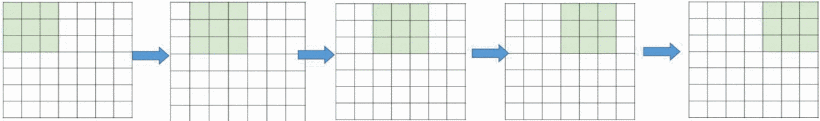
\includegraphics[width=0.7\textwidth]{images/CNN/fig_Stride.png}
            \caption{Esempio di movimento di un filtro $3 \times 3$ con stride 1. \cite{8308186}}
            \label{fig:Stride}
        \end{figure}
    
        \begin{figure}[h]
            \centering
            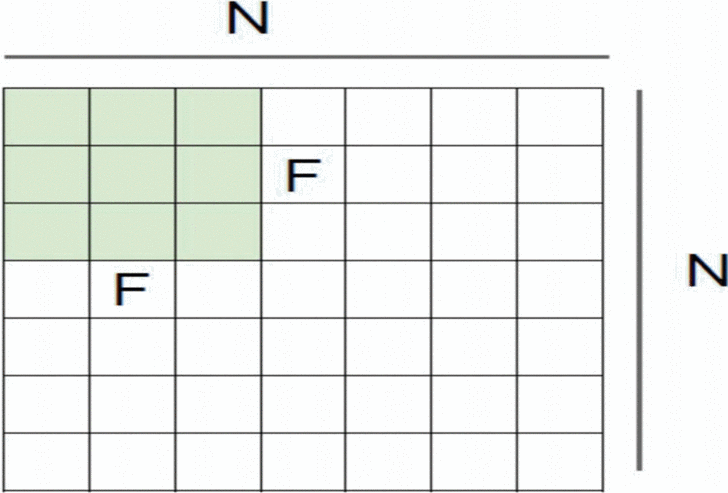
\includegraphics[width=0.7\textwidth]{images/CNN/fig_Stride2.png}
            \caption{Risultato dell'applicazione dello stride. \cite{8308186}}
            \label{fig:Stride2}
        \end{figure}

        \item[Padding] Uno degli svantaggi della fase di convoluzione è la perdita di informazioni che
        potrebbero esistere sul bordo dell'immagine, poiché durante la convoluzione i pixel del bordo sono 
        visti ed usati meno volte rispetto a quelli del centro, dato che il filtro li osserva solo quando 
        si muove attraverso l'immagine. Un metodo molto semplice ma efficace per risolvere il problema, è 
        usare zero-padding. L'altro vantaggio di zero-padding è quello di gestire la dimensione dell'output. 
        Per esempio, in Figura \ref{fig:Stride}, con $N=7$ e $F=3$ e stride 1, l'uscita sarà $5 \times 5$ 
        (che si restringe da un ingresso $7 \times 7$). Tuttavia, aggiungendo uno zero-padding, l'output 
        sarà $7 \times 7$, che è esattamente lo stesso dell'input originale (il valore attuale di $N$ 
        diventa 9, usata nella (1). L'equazione modificata che include zero-padding è la (2).
        \[ O=1+ \frac{N+2P-F}{S} \tag{2} \]
        dove $P$ è il numero dei livelli di riempimento applicati dallo zero-paddding (ad esempio $P=1$ in
        Figura \ref{fig:Padding}). Questa idea di riempimento ci aiuta a impedire che la dimensione dell'uscita
        di rete si restringa con la profondità. Pertanto, è possibile avere un numero qualsiasi di reti 
        convoluzionali profonde \cite{o2015introduction}.
    \end{description}

       \begin{figure}[h]
           \centering
           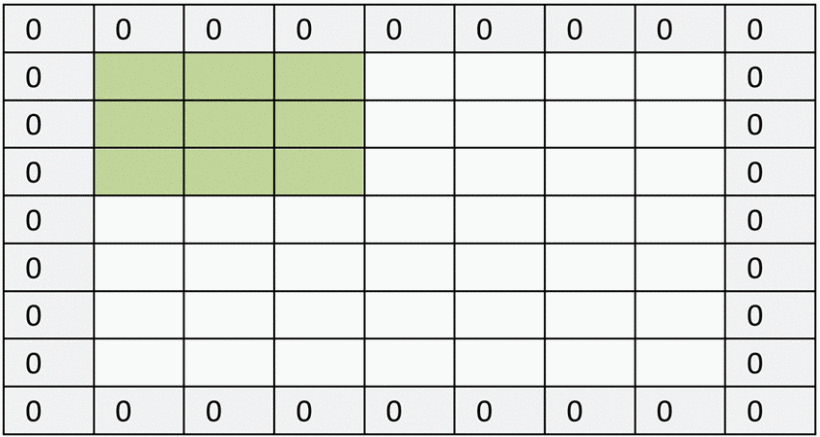
\includegraphics[width=0.7\textwidth]{images/CNN/fig_Padding.png}
           \caption{Effetto dello zero padding sull'immagine di input. \cite{8308186}}
           \label{fig:Padding}
       \end{figure}

    \begin{figure}[h]
        \centering
        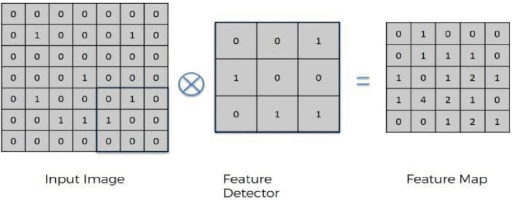
\includegraphics[width=0.7\textwidth]{images/ConvLayer_resize.png}
        \caption{Funzionamento della convoluzione \cite{9077735}}
        \label{fig:ConvKernel}
    \end{figure}
    
    \begin{figure}[h]
        \centering
        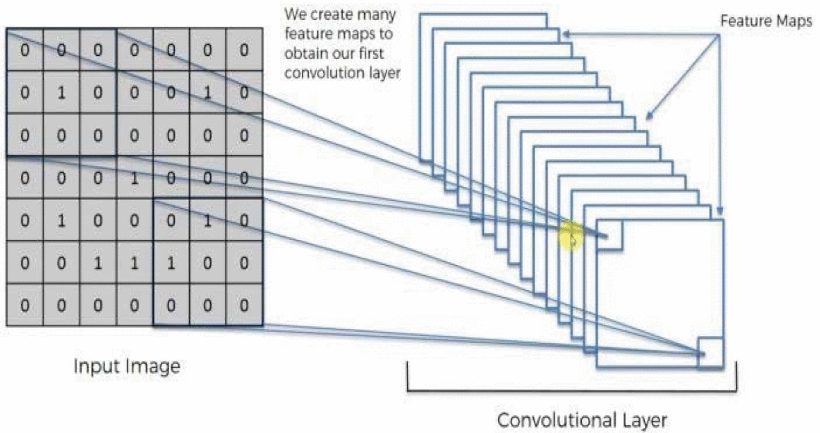
\includegraphics[width=0.7\textwidth]{images/CNN/ConvsLayer.png}
        \caption{Layer Convoluzionale \cite{9077735}}
        \label{fig:ConvLayer}
    \end{figure}
    \item[Pooling Layer] Il pooling è un passo importante per ridurre ulteriormente le dimensioni della mappa di
    attivazione, mantenendo solo le caratteristiche importanti e riducendo l'invarianza spaziale. Questo a sua 
    volta riduce il numero di caratteristiche apprendibili dal modello. Ciò aiuta a risolvere il problema del
    sovradimensionamento. Il pooling consente alla CNN di incorporare tutte le diverse dimensioni di un'immagine 
    in modo che la rete riconosca con successo l'oggetto dato anche se la sua forma è inclinata o è presente con
    un'angolazione diversa. 
    Ci sono vari tipi di pooling come il Max Pooling, l'Average Pooling, lo Stochastic Pooling e lo Spatial Pyramid
    Pooling. Tra questi, il più popolare è il Max Pooling che prende il valore più alto da ogni sub matrice della mappa 
    di attivazione e forma una matrice separata. In questo modo si assicura che le caratteristiche apprendibili
    rimangano limitate nel numero, preservando allo stesso tempo le caratteristiche chiave di qualsiasi immagine. 
    Il Max Pooling è solitamente fatto usando un filtro $2 \times 2$. La Figura \ref{fig:PoolLayer} mostra il
    funzionamento di tale layer.  
    \begin{figure}[h!]
        \centering
        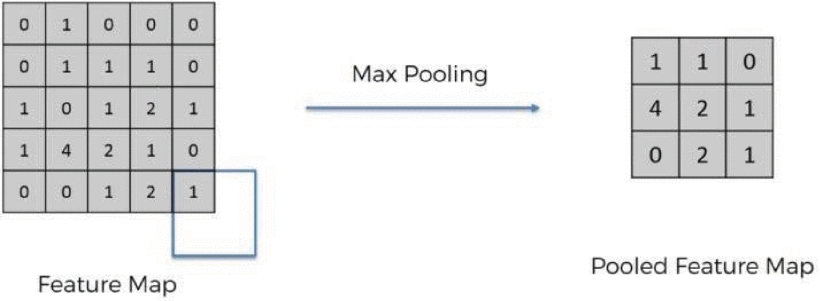
\includegraphics[width=0.7\textwidth]{images/PoolLayer.png}
        \caption{Applicazione Max Pooling \cite{9077735}}
        \label{fig:PoolLayer}
    \end{figure}
    \item[Batch Normalization layer] La Batch Normalization (BatchNorm) \cite{ioffe2015batch,9077735} è stata
    probabilmente una delle innovazioni architetturali di maggior successo nel deep learning e anche se la sua 
    efficacia è indiscutibile, non abbiamo una ferma comprensione del perché questo è il caso. In generale, 
    BatchNorm è un meccanismo che mira a stabilizzare la distribuzione (su un mini lotto) di input ad un
    determinato livello di rete durante l'addestramento. Ciò si ottiene aumentando la rete con strati aggiuntivi 
    che impostano i primi due momenti (media e varianza) della distribuzione di ciascuna attivazione rispettivamente 
    a $0$ (zero) e $1$ (uno). Poi, gli ingressi normalizzati batch sono in genere anche in scala e spostati sulla 
    base di parametri addestrabili per preservare l'espressività del modello. Questa normalizzazione viene applicata
    prima della non-linearità del layer precedente. Una delle motivazioni chiave per lo sviluppo di BatchNorm è 
    stata la riduzione del cosiddetto Spostamento Covariato Interno (Internal Covariate Shift).
    Questa riduzione è stata ampiamente considerata come il fulcro del successo di BatchNorm. Ioffe e Szegedy
    \cite{ioffe2015batch} descrivono l'ICS come "il fenomeno in cui la distribuzione degli input a un livello 
    della rete cambia a causa di un aggiornamento dei parametri dei livelli precedenti". Questo cambiamento porta 
    ad un costante spostamento del problema di formazione di base e si ritiene quindi che abbia un
    effetto negativo sul processo di training.
    \item[Drop-out Layer] Drop-out \cite{hinton2012improving} è un metodo per regolarizzare le reti neurali, 
    proposto per evitare l'over-fitting. È un metodo di regolarizzazione\footnote{Un metodo di regolarizzazione 
    è spesso formalmente definito come un metodo di inversione a seconda di un singolo parametro reale $\alpha \geq 0$
    che produce una famiglia di soluzioni approssimative $f(\alpha)$ con le seguenti due proprietà: 
    in primo luogo, per $\alpha$ grande abbastanza la soluzione regolarizzata $f(\alpha)$ è stabile a fronte di
    perturbazioni o rumore nei dati (a differenza della soluzione generalizzata) e, in secondo luogo, per $\alpha$ 
    che va a zero è recuperata la soluzione generalizzata non regolarizzata: $f(\alpha) = f() + \alpha \to 0$} 
    che imposta stocasticamente a zero le attivazioni delle unità nascoste per ogni caso di addestramento al momento
    della fase di training. 
    Questo interrompe il co-adattamento dei rilevatori di funzionalità poiché le unità degli strati nascosti 
    selezionati dal drop-out non possono influenzare le restanti unità. Un altro modo per interpretare il drop-out 
    è che produce una forma molto efficiente di media del modello in cui il numero di modelli addestrati è 
    esponenziale in quello delle unità, e questi modelli condividono gli stessi parametri. Il drop-out ha anche
    ispirato altri metodi stocastici come lo Stochastic Pooling \cite{zeiler2013stochastic} e 
    DropConnect \cite{wan2013regularization}. 
    Anche se il Drop-out è noto per funzionare bene in layer fully connected di reti neurali convoluzionali il 
    suo effetto non è stato ancora ben documentato \cite{wan2013regularization, zeiler2013stochastic,
    krizhevsky2017imagenet}.
    Il Drop-out è una nuova tecnica di regolarizzazione che è stata più recentemente impiegata nel deep learning. 
    È simile al bagging \cite{breiman1996bagging}, in cui un insieme di modelli sono addestrati su diversi sottoinsiemi
    degli stessi dati di allenamento. Al momento della prova, le previsioni dei diversi modelli sono mediate insieme.
    Nel bagging, ogni modello ha parametri indipendenti e tutti i membri sarebbero addestrati individualmente. 
    Nel caso di formazione tramite drop-out, ci sono esponenzialmente molti modelli eventualmente da
    addestrare ma non lo sono tutti in maniera palese, poiché questi ultimi condividono gli stessi parametri. 
    In realtà, il numero di modelli addestrati tramite drop-out non è più grande di $\gamma \times \epsilon$, 
    dove $\gamma$ è il numero di esempi di formazione, ed $\epsilon$ è il numero di epoche usate nel training. 
    Questo è molto più piccolo del numero di modelli eventualmente addestrati che è pari a $2^n$ 
    (dove $n$ è il numero di unità nascoste in una rete neurale feed-forward). Pertanto, la stragrande maggioranza 
    dei modelli non sono esplicitamente addestrati al momento della formazione.
    \item[Fully Connected Layer] Questo è il layer che viene utilizzato alla fine della rete neurale. 
    Generalmente la matrice dei pesi viene appiattita prima di essere passata ai neuroni. È difficile seguire i 
    dati dopo questo punto a causa della presenza di molte unità nascoste con peso variabile all'uscita di ogni 
    neurone. Tutto il ragionamento e il calcolo sui dati ed il raggiungimento di una target class associato al 
    nostro input, viene delegato a questa tipologia di layer.
\end{description}

\subsubsection{Funzioni d'attivazione}~\newline
\label{subsubsec:act_func}
Le CNN possono sfruttare diverse funzioni di attivazione per esprimere funzioni complesse. Simile alla funzione del
modello del neurone del cervello umano, la funzione di attivazione qui è un'unità che determina quale informazione
dovrebbe essere trasmessa al neurone seguente.
Ogni neurone nella rete neurale accetta il valore di uscita dei neuroni dal livello precedente come input e passa il
valore elaborato al livello successivo.
In una rete neurale multilayer, la funzione di attivazione è posta tra due layer e la struttura 
è mostrata nella figura \ref{fig:activation_func}.
\begin{figure}[h!]
    \centering
    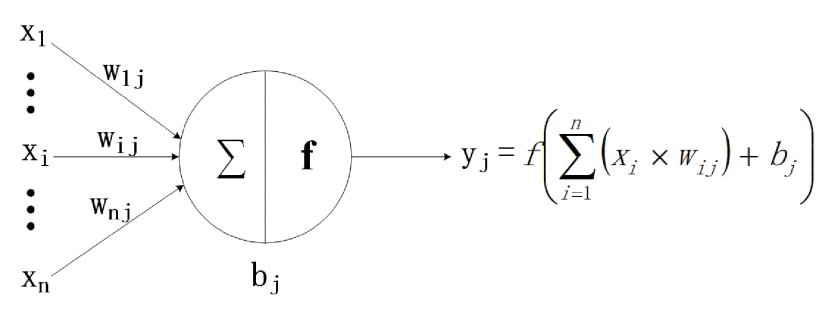
\includegraphics[width=\textwidth]{images/activaiton_func.png}
    \caption{Diagramma generale sulle funzioni d'attivazione \cite{9451544}}
    \label{fig:activation_func}
\end{figure}
In Figura \ref{fig:activation_func} , $x_{i}$ rappresenta la funzione di input; $n$ sono le caratteristiche in input 
al neurone $j$ allo stesso tempo; $W_{ij}$ rappresenta il valore di peso della connessione tra la funzione di input
$x_{i}$ e il neurone $j$; $b_{j}$ rappresenta lo stato interno del neurone $j$, che è il valore di bias; 
e $y_{j}$ è l'uscita del neurone $j$. $f()$ è la funzione di attivazione, che può essere la funzione sigmoide, 
la funzione Tanh \cite{726791} o l'unità lineare rettificata (ReLU) \cite{nair2010rectified}.
Se non viene utilizzata una funzione di attivazione o viene utilizzata una funzione lineare, l'input di ciascun 
livello sarà una funzione lineare dell'output del livello precedente. In questo caso, He et al. \cite{he2015delving}
dimostrano che non importa quanti layer ha la rete neurale, l'output sarà sempre una combinazione lineare dell'input, 
il che significa che i livelli nascosti non hanno effetto. Questa situazione rappresenta il modello del 
perceptron \cite{rosenblatt1958perceptron, rosenblatt1961principles}, che ha capacità di apprendimento limitata. 
Per questo motivo, le funzioni non lineari sono introdotte come funzioni di attivazione. Teoricamente, reti 
neurali profonde con funzioni di attivazione non lineari possono approssimare qualsiasi funzione, il che 
migliora notevolmente la capacità delle reti neurali di adattarsi ai dati.
La funzione sigmoide è una delle più tipiche funzioni di attivazione non lineari con una forma S complessiva (
vedere Figura \ref{fig:activation_function}(a)). 
Quando il valore $x$ si avvicina a $0$, il gradiente diventa più ripido. La funzione sigmoide può mappare un 
numero reale nell'intervallo $(0, 1)$, pertanto, può essere utilizzata per problemi di classificazione binaria. 
Inoltre, i modelli Senet \cite{hu2018squeeze} e MobileNet v3 \cite{howard2019searching} devono trasformare il 
valore di uscita di ogni layer in $(0, 1)$ per poter usare il loro meccanismo di attenzione. 
In questo contesto la sigmoide è la funzione più appropriata da implementare.
Diversamente dalla sigmoide, la funzione Tanh \cite{726791} (vedere Figura \ref{fig:activation_function}(b)) 
può mappare un numero reale nel range $(-1, 1)$. Poiché il valore medio dell'output di Tanh è $0$, può raggiungere 
una sorta di normalizzazione. Questo rende l'apprendimento di nuove complessità più facili per lo
strato successivo.
Oltre Tanh, esiste anche ReLU \cite{nair2010rectified} (vedere Figura \ref{fig:activation_function}(c)) che 
risulta essere un'altra funzione di attivazione efficace. 
Quando $x$ è inferiore a $0$, il suo valore di funzione è $0$; quando $x$ è maggiore o uguale a $0$, il suo valore 
di funzione è $x$ stesso. 
Rispetto alla funzione sigmoide e alla funzione Tanh, un vantaggio significativo dell'utilizzo della funzione ReLU è che 
può accelerare l'apprendimento. Sigmoide e Tanh mentre calcolano i derivati coinvolgono nel calcolo una funzione
esponenziale che include la divisione.
Il derivato di ReLU, invece, è una costante. Inoltre, nella funzione sigmoide e Tanh, se il valore di $x$ è troppo
grande o troppo piccolo, il gradiente della funzione è piccolo, il che può far convergere lentamente la funzione. 
Tuttavia, quando $x$ è inferiore a $0$, il derivato di ReLU è $0$, e quando $x$ è maggiore di $0$, la derivata è $1$;
quindi, si può ottenere un effetto di convergenza ideale. AlexNet \cite{krizhevsky2017imagenet}, il miglior modello 
in ILSVRC-2012, utilizza ReLU come funzione di attivazione del modello basato su CNN perché mitiga il problema della
scomparsa del gradiente quando la rete è profonda e verifica che l'uso di ReLU superi il sigma nelle reti profonde.

\begin{figure}[h!]
    \centering
    \subfloat[][]{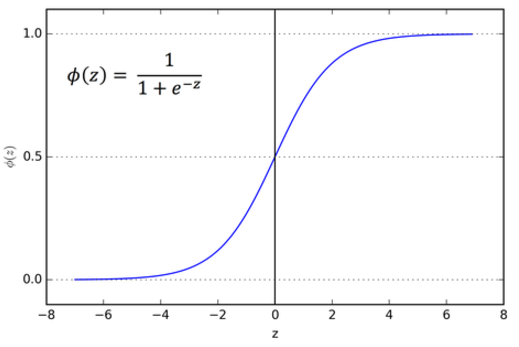
\includegraphics[scale=0.6]{images/ActivationFunction/sigmoid_function.png}} \hfill % 1
		\subfloat[][]{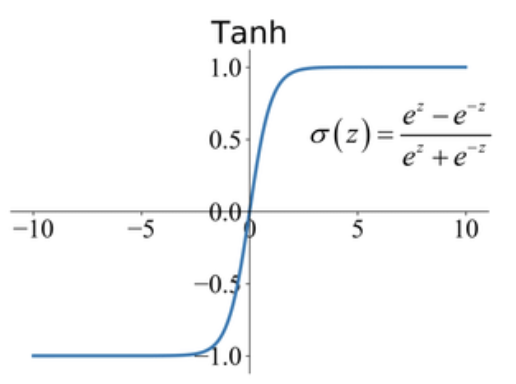
\includegraphics[scale=0.6]{images/ActivationFunction/Tanh_function.png}} \hfill % 2
		\subfloat[][]{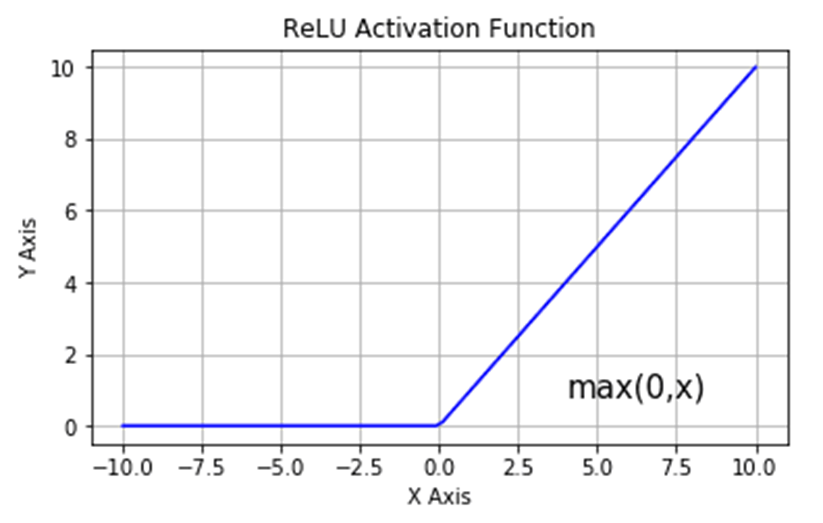
\includegraphics[scale=0.6]{images/ActivationFunction/ReLU_function.png}} \hfill % 3
    \caption{Esempi di funzioni d'attivazione: (a) Sigmoid, (b) Tanh, (c) ReLU}
    \label{fig:activation_function}
\end{figure}

Sulla base della discussione precedente, notiamo che ReLU non include il limite superiore. In pratica, 
possiamo impostare un limite superiore, come ReLU6 \cite{krizhevsky2010convolutional}.

\begin{figure}
    \centering
    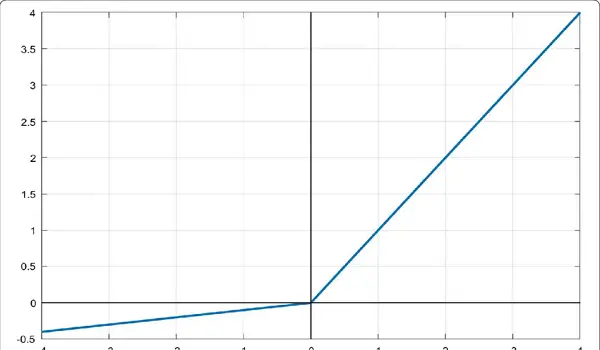
\includegraphics[width=0.7\textwidth]{images/leaky-ReLU-activation-function-new.png}
    \caption{La funzione Leaky ReLU}
    \label{fig:leaky_relu}
\end{figure}
Tuttavia un difetto di ReLU è che, quando $x$ è minore di $0$, il gradiente di ReLU è $0$. Ciò significa che 
l'errore retropropagato verrà moltiplicato per $0$, con il risultato che non verrà passato alcun errore al livello
precedente.
In questo scenario, i neuroni possono essere considerati inattivati o morti.
Pertanto, vengono proposte alcune versioni migliorate. Un esempio è Leaky ReLU (Figura \ref{fig:leaky_relu}) che riesce 
a ridurre l'inattivazione dei neuroni.
Quando $x$ è minore di $0$, l'errore retropropagato è $x/a$, invece di zero, dove $a$ è un parametro fisso
nell'intervallo $(1, +\infty)$.

\subsubsection{Funzioni di perdita}~\newline
\label{subsubsec:loss}
La funzione di perdita o la funzione di costo è sfruttata per calcolare la distanza fra il valore previsto ed il 
valore reale. La funzione di perdita è usata solitamente come criterio imparante del problema di ottimizzazione. 
La funzione di perdita può essere utilizzata con CNN per affrontare i problemi di regressione e i problemi di
classificazione, il cui obiettivo è quello di minimizzare la funzione stessa. Le funzioni di perdita comunemente usate
includono l'errore assoluto medio (MAE), l'errore quadratico medio (MSE), l'entropia trasversale e così via. 
Nelle CNN, ci sono molte funzioni di perdita da gestire quando si tratta di un task di classificazione. La più
conosciuta ed usata è la Cross-Entropy, che è usata per valutare la differenza tra la distribuzione di probabilità
ottenuta dall'allenamento corrente e la distribuzione effettiva. 
Questa funzione confronta la probabilità prevista con il valore di uscita effettivo ($0$ o $1$) in ogni classe 
e calcola il valore di penalità in base alla distanza da loro. La penalità è logaritmica, pertanto, la funzione 
fornisce una penalità minore ($0.1$ o $0.2$) per differenze più piccole tra le due distribuzioni e una penalità 
più grande ($0.9$ o $1.0$) per differenze più grandi.
La Cross-Entropy loss function è anche chiamata perdita di Softmax, poiché viene usata nelle reti convoluzionali 
in combinazione con un layer Softmax.
Ad esempio, AlexNet \cite{krizhevsky2017imagenet}, Inception v1 \cite{szegedy2015going} e Resnet \cite{he2016deep}
utilizzano la Cross-Entropy loss function come funzione di perdita nei loro articoli originali e ciò li ha aiutati 
a raggiungere risultati all'avanguardia. Tuttavia, la Cross-Entropy loss function ha alcuni difetti: essa si 
preoccupa solo della correttezza della classificazione ma non del grado di compattezza all'interno della stessa
classe o del margine tra classi diverse. 
Una delle varianti della Cross-Entropy è la Large-Margin Softmax loss \cite{liu2016large}. Lo scopo di questa 
funzione è di massimizzare la densità interna tra campioni di una stessa classe e massimizzare la distanza tra 
classi diverse. 
La Large-Margin Softmax loss aggiunge un margine tra classi diverse e introduce la regolarità di tale margine 
attraverso l'angolo della matrice del peso di vincolo. Tale funzione è stata utilizzata per face recognition 
\cite{liu2016large}, emotion recognition \cite{tan2017group}, speaker verification \cite{liu2019large}, e così via.

\subsubsection{Ottimizzatori}~\newline
\label{subsubsec:optimizer}
Nelle CNN, spesso abbiamo bisogno di ottimizzare le funzioni non convesse. I metodi matematici richiedono un'enorme
potenza di calcolo, pertanto, gli ottimizzatori vengono utilizzati nel processo di allenamento per ridurre al minimo 
la funzione di perdita e per ottenere parametri di rete ottimali in un tempo accettabile. Gli algoritmi di
ottimizzazione comuni includono momentum, Root-mean-square prop (RMSprop), stima del momento adattivo (Adam), e
così via. Ciascuno dei precedenti algoritmi si basa sulla discesa del gradiente e ne esistono tre tipi che si possono
utilizzare per allenare i modelli di CNN:
\begin{enumerate}
    \item Batch Gradient Descent (BGD)
    \item Stochastic Gradient Descent (SGD)
    \item mini-BGD (MBGD)
\end{enumerate}
Il BGD indica che un intero lotto di dati deve essere calcolato per ottenere un gradiente per ogni aggiornamento al
fine di garantire la convergenza all'ottimo globale del piano convesso e all'ottimo locale del piano non convesso.
Tuttavia, BGD è troppo lento da usare perché deve essere calcolato il gradiente medio dei campioni interi del lotto.
Inoltre, può essere difficile per i dati che non sono adatti per il calcolo in memoria. BGD, quindi, è difficilmente
utilizzato nella pratica nella formazione di modelli basati su CNN. Al contrario, SGD utilizza un solo
campione per ogni aggiornamento. È evidente che il tempo di SGD per ogni aggiornamento è notevolmente inferiore 
rispetto a BGD perché soltanto un gradiente del campione totale viene usato per il calcolo. In questo caso, SGD è 
adatto per l'apprendimento online \cite{saad1999line}. Tuttavia, SGD è rapidamente aggiornato con varianza elevata 
e ciò causa una forte oscillazione nella funzione di perdita.
Da un lato, l'oscillazione del calcolo può far saltare il calcolo del gradiente dall'ottimo locale e infine 
raggiungere un punto migliore.
D'altra parte, SGD non può mai convergere a causa dell'oscillazione infinita. In termini di tasso di convergenza,
supponendo che la deviazione standard di ciascun campione per la distribuzione reale sia $\sigma$, la deviazione
standard di $n$ campioni è $\frac{\sigma}{\sqrt{n - 1}}$. 
Quando usiamo i campioni per stimare il gradiente, un campione introduce una deviazione standard pari a $\sigma$,
ma usandone $n$ ciò non fa diminuire linearmente la deviazione standard. L'unica cosa che aumenta è la quantità 
di calcolo sugli $n$ campioni e l'aumento è lineare. 
Sulla premessa di questa stessa quantità di calcolo, la velocità di convergenza dell'utilizzo dell'intero set di
campioni è molto più lenta rispetto all'utilizzo di un piccolo numero di campioni. In altre parole, per convergere
nello stesso punto ottimale, quando si utilizza l'intero set di allenamento, anche se il numero di iterazioni è 
piccolo, il tempo di ogni iterazione è lungo. Quindi, il costo totale di tempo è maggiore rispetto 
ad un piccolo numero di campioni per più iterazioni multiple.

Teoricamente, quanto affermato prima è vero, ossia minore è il numero di campioni, più veloce sarà il tasso 
di convergenza quando si utilizza una CPU single-core. Tuttavia, quando si utilizzano le GPU per l'addestramento, 
a causa del gran numero di core ed all'eccellente capacità di calcolo parallelo della GPU, ci vuole lo stesso 
tempo sia per calcolare un campione sia per calcolarne decine o centinaia. 
Pertanto, nella pratica ingegneristica basata su BGD e SGD, MBGD è stato proposto e utilizzato frequentemente. 
Esso combina i vantaggi di BGD e SGD e la dimensione del batch dipende dalla memoria della GPU e dal core di calcolo. 
MBGD utilizza un piccolo lotto di campioni per ogni aggiornamento in modo che possa non solo eseguire la discesa 
del gradiente in modo più efficiente di BGD, ma anche ridurre la varianza rendendo la convergenza più stabile.

Molti modelli classici della CNN utilizzano MGBD per addestrare le loro reti, come AlexNet
\cite{krizhevsky2017imagenet}, VGG \cite{simonyan2014very}, inception v2 \cite{szegedy2015going}, 
Resnet \cite{krizhevsky2017imagenet} e DenseNet \cite{huang2017densely}.
È stata inoltre utilizzata in FaceNet \cite{schroff2015facenet}, DeepID \cite{sun2014deep} e DeepID2 \cite{sun2014deeps}.
Sulla base di MBGD, sono stati proposti una serie di algoritmi efficaci per l'ottimizzazione per accelerare il 
processo di formazione del modello. Qui di seguito mostriamo alcuni ottimizzatori che si basano MBDG:

\begin{itemize}
    \item  L'algoritmo di Adagrad \cite{duchi2011adaptive} è un altro algoritmo di ottimizzazione basato sui gradienti.
           Può adattare dinamicamente il learning rate ai parametri delle rete, cioè esegue piccoli aggiornamenti 
           (se ad esempio, sussiste un basso learning rate) per caratteristiche che si mostrano con alta frequenza 
           ed esegue aggiornamenti più ampi (cioè, con un alto learning rate) per quelle non frequenti. 
           Pertanto, è adatto per l'elaborazione di dati sparsi. Uno dei principali vantaggi di Adagrad è che non è 
           necessario regolare manualmente il tasso di apprendimento. 
           Nella maggior parte dei casi, si usa solo $0.01$ come learning rate predefinito \cite{ma2018shufflenet}. 
           Ad esempio FaceNet \cite{schroff2015facenet} utilizza Adagrad come ottimizzatore in allenamento.

    \item L'algoritmo di Adadelta \cite{zeiler2012adadelta}, che è un'estensione dell'Adagrad, è progettato per 
          ridurre il suo learning rate come una funzione monotona descrescente.
          Non si limita ad accumulare tutti i gradienti al quadrato, ma imposta una finestra di dimensioni fisse 
          per limitare il numero di gradienti al quadrato accumulati. Allo stesso tempo, la somma dei gradienti 
          è definita ricorsivamente come la media di decadimento di tutti i gradienti precedentemente quadrati,
          piuttosto che memorizzare direttamente i gradienti precedentemente quadrati. L'algoritmo Adadelta è 
          sfruttato in molti compiti come speech recognition e sentence classification \cite{chorowski2015attention,
          kim-2014-convolutional}.

    \item L'algoritmo RMSprop \cite{hinton2012neural} è progettato per risolvere il problema del tasso di 
          apprendimento radicalmente decrescente nell'algoritmo Adagrad. MobileNet \cite{howard2017mobilenets}, 
          versione iniziale v3 \cite{szegedy2016rethinking} e versione iniziale v4 \cite{szegedy2017inception} 
          hanno ottenuto i migliori modelli utilizzando RMSprop.

    \item Un altro ottimizzatore utilizzato di frequente è la stima adattiva del momento (Adam) \cite{kingma2014adam}. 
          È essenzialmente un algoritmo formato combinando la quantità di moto con l'RMSprop. Adam memorizza 
          sia la media di decadimento esponenziale dei gradienti quadrati passati, come l'algoritmo Adadelta, 
          sia la media di decadimento esponenziale medio dei gradienti passati, come l'algoritmo di quantità di moto. 
          La pratica ha dimostrato che l'algoritmo Adam funziona bene su molti problemi ed è applicabile a molte 
          strutture diverse di CNN \cite{sharma2015action,van2018predicting}.

          L'algoritmo AdaMax \cite{kingma2014adam} è una variante di Adam che semplifica l'intervallo di confine 
          del tasso di apprendimento ed è stato utilizzato per addestrare i modelli CNN di \cite{van2018predicting} e
          \cite{niklaus2017video}.

          La stima di Adam accelerata da Nesterov (Nadam) \cite{dozat2016incorporating} è una combinazione di Adam 
          e NAG. Nadam ha un vincolo più forte sul tasso di apprendimento e un impatto diretto sull'aggiornamento 
          del gradiente. Nadam è utilizzato in molti compiti come la classificazione del livello del suono in un 
          luogo \cite{nguyen2018convolutional,schindler2018multi}.
\end{itemize}

\subsubsection{Hyperparameter tuning}~\newline
Quando si costruisce una CNN, oltre a selezionare la funzione di attivazione, la funzione di perdita e l'ottimizzatore,
dobbiamo anche regolare molti altri iperparametri che influiscono notevolmente sulle prestazioni del modello. Come è
noto, non esiste un insieme fisso di iperparametri in grado di garantire una soluzione ottimale per tutto il tempo. 
Per cui, un insieme di esperienze e buone regole pratiche sono significative durante l'hyperparameter tuning. 
Un modello di deep neural network (DNN) apprende i valori appropriati delle sue variabili di configurazione, 
cioè i pesi di connessione e il bias, dai dati di allenamento e, tali variabili, sono chiamate parametri
\cite{nasrabadi2007pattern}. 
Il processo di determinazione dei loro valori dai dati è noto come formazione o apprendimento del modello.
Tuttavia, ci sono alcuni parametri di alto livello noti come "iperparametri" i cui valori non possono essere 
appresi dai dati \cite{bergstra2011algorithms}. Alcuni degli iperparametri importanti per le architetture DNN 
includono il numero di layer, il numero di nodi, il tasso di apprendimento, il tasso di regolarizzazione, 
la funzione di perdita, la funzione di attivazione, il metodo di ottimizzazione, il metodo di valutazione, ecc.
L'addestramento di una DNN è un processo relativamente ingombrante poiché queste ultime devono essere
addestrate con una grande quantità di dati per imparare i loro parametri con precisione \cite{lecun2015deep,
schmidhuber2015deep}. 
Anche una singola istanza del problema di formazione della rete neurale potrebbe richiedere giorni o addirittura
settimane per allenarsi. Ciò influenza anche le reti neurali convoluzionali (CNN) distribuite per riconoscere le
immagini e video \cite{pmlr-v9-glorot10a}.
Quando la CNN tenta di riconfigurare i suoi parametri dopo l'introduzione di piccoli rumori, si rischia 
l'over-fitting e il rallentamento della convergenza del modello \cite{7536654}. Allo stesso modo, 
l'addestramento delle reti neurali ricorrenti (RNN) è un compito difficile poiché hanno un'architettura 
complessa e soffrono di problemi di gradienti che svaniscono \cite{Pascanu2013}.
Le prestazioni di formazione delle DNN e la loro struttura dipendono fortemente dalle scelte dei valori 
degli iperparametri \cite{Dobslaw2010APF}.
Perciò, decidere i valori ottimali degli iperparametri è essenziale per esprimere il massimo potenziale dei modelli 
DNN \cite{7536654}. 
La Tabella \ref{tab:Hyper_tab} a pagina \pageref{tab:Hyper_tab} mostra come alcuni iperparametri comuni influenzano le prestazioni dei modelli.
\begin{table}[hpbt!]
    \centering
    \caption{Iperparametri più comuni}
    \footnotesize
    \begin{tabular}{>{\bfseries}lp{0.50\textwidth}l}
    \toprule
        Iperparametri & Descrizione \\
        \midrule
         Learning rates &  Il tasso di apprendimento si riferisce alla dimensione del passo di aggiornamento dei pesi di
         rete. Può essere costante o variabile. Come accennato nella sottosezione Ottimizzatori
         \ref{subsubsec:optimizer}, gli algoritmi di ottimizzazione determinano diversi tassi di apprendimento. Per
         rendere la discesa in pendenza migliore, il valore della velocità di apprendimento dovrebbe essere impostato 
         in un intervallo appropriato. Se la velocità di apprendimento è troppo piccola, la velocità di convergenza 
         sarà lenta; se è troppo grande, i parametri oscilleranno avanti e indietro su entrambi i lati della soluzione
         ottimale. \\
         \midrule
         Epoch & L'epoca si riferisce al numero di volte che tutto l'insieme di addestramento è dato in input 
         alla rete neurale per il training. Quando il divario di accuratezza fra l'insieme di addestramento e l'insieme
         di convalida è piccolo, l'epoca corrente è considerata appropriata. Altrimenti, se il divario diminuisce,
         significa che l'epoca è troppo piccola, con conseguente under-fitting; se il divario aumenta, l'epoca è 
         troppo grande, con conseguente over-fitting.\\  
         \midrule
         Mini-batch size & La dimensione del lotto mini è il numero di campioni inviati al modello in ogni allenamento.
         Nel processo di ottimizzazione della rete, avere la dimensione del batch troppo piccola significa che il numero
         di campioni immessi nella rete è troppo piccolo, cioè non rappresentativo, e il rumore aumenta di conseguenza,
         il che rende la convergenza della rete molto difficoltosa. La dimensione del lotto troppo grande rende la
         direzione del gradiente quasi stabile e ciò rende la discesa del gradiente rapida verso un punto ottimale
         locale o sella locale.\\
         \midrule
         Number of conv layers e conv kernels & Ogni livello Conv di solito contiene caratteristiche di livello diverso.
         Gli strati superficiali possono rilevare le caratteristiche dei bordi, le caratteristiche locali e altre
         caratteristiche a basso livello dell'immagine, mentre gli strati profondi possono rilevare le caratteristiche
         globali. Di solito, le reti con più livelli e kernel hanno la capacità di rappresentare caratteristiche più
         complesse, ma nel frattempo, sono più difficili da addestrare. \\
         \midrule
         Size of conv kernels & Sulla premessa dello stesso campo ricettivo, più piccolo è il kernel di convoluzione,
         meno sono i parametri e meno complessità computazionale è richiesta. In particolare, quando la dimensione del
         kernel di convoluzione è maggiore di $1$, può aumentare il campo ricettivo. Se si usa il kernel di convolutione
         con dimensione pari, anche se il padding viene aggiunto simmetricamente, non possono essere mantenute invariate
         la dimensione della mappa delle caratteristiche di input e la dimensione della mappa delle caratteristiche di
         output .\\
         \bottomrule
    \end{tabular}
    \normalsize
    \label{tab:Hyper_tab}
\end{table}

\subsection{Generazione delle Heatmap}~\newline
Le heatmap sono generate sulla base dell'idea di Guided Grad-CAM \cite{selvaraju2017grad}. Come premessa bisogna usare
solo il dataset di training sulla rete CNN già addestrata, in seguito, per ogni campione di dati, si è riportato la
mappa di attivazione dell'ultimo layer convoluzionale durante il processo di forward passing.
Poi, attraverso il processo di backpropagation, abbiamo registrato i gradienti specifici dell'etichetta di ogni neurone
dell'ultimo layer convoluzionale. Questi gradienti rappresentano il contributo dei neuroni ai risultati della
classificazione. La Grad-CAM viene calcolata utilizzando una somma ponderata delle mappe di attivazione che viene 
poi ridimensionata alle dimensioni dell'input. Per migliorare ulteriormente l'accuratezza della localizzazione, i
gradienti del layer di input sono moltiplicati con la Grad-CAM, generando infine la Guided Grad-CAM per ciascun
campione, che può essere visualizzata come una heatmap. 
Successivamente, è stata calcolata la media di tutte le heatmap della stessa classe e, dopo la normalizzazione, sono
state ottenute le heatmap per ogni classe. L'intensità di ciascun pixel rappresenta il significance score del gene 
che corrisponde al contributo dato da quest'ultimo alla classificazione.
In realtà, questo processo di generazione delle heatmap potrebbe essere impiantato nell'addestramento della rete 
neurale convoluzionale poiché non influisce sul processo di addestramento e di test.
La computazione è, però, minore con il metodo a due fasi descritto precedentemente, poiché la Grad-CAM richiede che
tutti i campioni passino una sola volta attraverso la rete neurale.

\subsubsection{Gradient Classification Activation Map}~\newline
Un certo numero di opere precedenti hanno affermato che rappresentazioni più profonde in una CNN catturano costrutti
visivi di livello superiore \cite{bengio2013representation, mahendran2016visualizing}. Inoltre, le caratteristiche
convoluzionali mantengono naturalmente le informazioni spaziali che vengono perse nei layer fully connected, quindi
possiamo aspettarci che gli ultimi layer convoluzionali abbiano il miglior compromesso tra semantica di alto livello 
e informazioni spaziali dettagliate.
I neuroni in questi layer cercano nell'immagine informazioni semantiche specifiche della classe (ad esempio, parti di
oggetti). Grad-CAM usa le informazioni di gradiente che fluiscono nell'ultimo strato convoluzionale della CNN per 
capire l'importanza di ogni neurone per una decisione di interesse. Anche se la nostra tecnica è molto generica e 
può essere utilizzata per visualizzare qualsiasi attivazione in una rete profonda, in questo lavoro ci concentriamo
sulla spiegazione delle decisioni che la rete può prendere eventualmente.

Come mostrato in Figura \ref{fig:GuidedGCam} a pagina \ref{fig:GuidedGCam}, al fine di ottenere la mappa di
localizzazione classe-discriminante Grad-CAM del layer $L$ definita come 
$L_{\text{Grad}-\text{CAM}}^{c}\in \mathbb{R}^{u \times v}$ di larghezza $u$ e altezza $v$ per qualsiasi classe $c$, 
in primo luogo calcoliamo il gradiente del punteggio per la classe $c$, $y^{c}$ (prima del Softmax), rispetto alla 
mappa delle caratteristiche $A^{k}$ di uno strato convoluzionale,cioè  $\frac{\partial y^{c}}{\partial A^{k}}$. 
Questi gradienti che scorrono indietro sono raggruppati nella media globale per ottenere i pesi 
$\alpha^{c}_{k}$ dell'importanza dei neuroni:
\[
    \alpha_{k}^{c}=\overbrace{\frac{1}{Z}\sum_{i}\sum_{j}}^{\text{global average pooling}}
    \underbrace{\frac{\partial y^{c}}{\partial A_{ij}^{k}}}_{\text{gradients via backprop}}\tag{1}
\]

Questo peso $\alpha^{c}_{k}$ rappresenta una linearizzazione parziale della rete profonda a valle di $A$, e 
cattura l'importanza della mappa caratteristica $k$ per una classe target $c$.

Eseguiamo una combinazione ponderata di mappe di attivazione in avanti e applichiamo ReLU per ottenere:
\[
    L_{\text{Grad}-\text{CAM}}^{c}=ReLU\underbrace{\left(\sum_{k}\alpha_{k}^{c}A^{k}\right)}_{\text{linear
    combination}}\tag{2}
\]

Si noti che ciò comporta una heatmap grossolana delle stesse dimensioni delle mappe delle caratteristiche 
convoluzionali ($14 \times 14$  nel caso degli ultimi strati convoluzionali della rete VGG \cite{simonyan2014very} 
e AlexNet \cite{krizhevsky2017imagenet}). 
Gli studi di ablazione e più visualizzazioni di Grad-CAM possono essere trovati in \cite{selvaraju2016grad}. 
In generale, $y^{c}$ non deve essere il punteggio di classe prodotto da una classificazione di immagine tramite CNN.
Potrebbe essere un'attivazione differenziabile che include parole da una didascalia o la risposta a una domanda.

\subsubsection{Guided BackPropagation}~\newline
Parte del potere d'interpretazione visiva di Guided Grad-CAM è ottenuta utilizzando l'algoritmo di Guided
Backpropagation basato sul gradiente (GBP) \cite{springenberg2014striving}, che si concentra sui pixel rilevanti 
delle immagini, responsabili della previsione della tipologia tumorale, fornendo un punteggio di confidenza a 
ciascun pixel. L'algoritmo GBP esegue una propagazione in avanti attraverso il modello in cui l'input viene passato
attraverso la funzione di attivazione ReLU, come descritto nell'Equazione \ref{eq:3}. Qui l'input $z_{i}^{l}$
rappresenta il punteggio di attribuzione per ogni timestamp. In questo caso, l'ingresso $z_{i}^{l}$ rappresenta 
l'uscita dell'$i^{th}$ neurone dell'$l^{th}$ strato. Durante la propagazione all'indietro, le saliency map ottenute 
con il filtro di convoluzione passano solo i valori che sono stati positivi durante il passaggio in avanti e
tagliano il resto dei valori. Ciò è visibile nell'Equazione \ref{eq:4}. Il segnale di errore $E_{i}^{l+1}$ 
rappresenta l'errore proveniente dall'$i^{th}$ neurone dello strato $(l+1)^{th}$. Il GBP modifica la propagazione
all'indietro classica, aggiungendo un'ulteriore condizione: passano solo i valori che sono stati positivi durante 
la propagazione in avanti e all'indietro. Dunque, dato questo vincolo viene generato un nuovo segnale di errore che 
tiene conto sia di $z_{i}^{l}$ sia di $E_{i}^{l+1}$ prima di passare l'errore al livello precedente, come descritto
nell'Equazione \ref{eq:5}. Pertanto, il gradiente è guidato dall'input dello strato precedente e dal segnale di 
errore dello strato successivo. I gradienti retropropagati evidenziano solo i pixel che influenzano fortemente la
diagnosi sulla tipologia di coorte tumorale, mentre la retropropagazione convenzionale non maschera le voci
negative durante la propagazione all'indietro. Il GBP calcola la versione vincolata del gradiente rispetto all'input,
mantenendo costante la matrice dei pesi della rete $\theta$ e utilizzando ReLU. Essendo una tecnica interpretabile a
posteriori, GBP non influenza la capacità decisionale del modello.

\begin{gather*} 
z_{i}^{l+1}=ReLU(z_{i}^{l})=max(z_{i}^{l},\ 0)\tag{3} \label{eq:3} \\ 
E_{i}^{l}=E_{i}^{l+1}\ \forall\ (z_{i}^{l} > 0),\ where\ E_{i}^{l+1}= \frac{\delta z^{out}}{\delta z_{i}^{l+1}}\tag{4} \label{eq:4}\\ E_{i}^{l}=E_{i}^{l+1}\ \forall\ (z_{i}^{l} > 0)\ and\ (E_{i}^{l+1} > 0)\tag{5} \label{eq:5}\\
\end{gather*}

\subsubsection{Guided GradCam}~\newline
Mentre le visualizzazioni Grad-CAM sono class-discriminant e localizzano bene le regioni più rilevanti in un'immagine,
esse non hanno la capacità di mostrare l'importanza a grana fine come i metodi di visualizzazione gradient pixel-space
transformation (ad es. guided backpropagation e deconvolution).
Per esempio, in Figura \ref{fig:GuidedGCam} a pagina \pageref{fig:GuidedGCam}, si può notare come nell'immagine 
indicata con \textbf{Grad-CAM}, vengano facilmente localizzate le regioni rilevanti del gatto; tuttavia, non è chiaro
dalle basse risoluzioni della heatmap perché la rete prevede questa particolare istanza come "gatto tigre".
Al fine di combinare gli aspetti migliori di entrambi, si fondono entrambi questi metodi di visualizzazione, Guided
Backpropagation e Grad-CAM, tramite moltiplicazione puntiforme ($L_{Grad-CAM}^{c}$ prima di essere moltiplicata 
con i gradienti generati da GBP viene ridimensionata alla risoluzione dell'immagine di ingresso utilizzando
interpolazione bi-lineare). Nella Figura \ref{fig:GuidedGCam} si può notare nell'immagine etichettata come
\textbf{Guieded Grad-CAM} come la heatmap generata con il procedimento descritto in precedenza sia ad alta risoluzione
e classe discriminante (ossia quando la classe di interesse è "gatto tigre", oltre che identificare importanti
caratteristiche del "gatto tigre", come strisce, orecchie a punta e gli occhi mostra anche la corretta tipologia 
di animale, cioè "gatto tigre" e non un altra classe). 
La sostituzione di Guided Backpropagation con Deconvolution, in base a quanto descritto sopra, dà risultati simili. 
Di fatti in \cite{lyu2018deep} hanno constato, però, che Deconvolution aveva degli artefatti: un vincolo
sull'architettura della rete presa in analisi e che le visualizzazioni erano rumorose rispetto a Guided
Backpropagation che erano generalmente meno rumorose. Per tali motivi, quindi, viene scelta come tecnica di 
gradient pixel-space transformation, Guided Backpropagation al posto di Deconvolution.
 \begin{figure}[h]
            \centering
            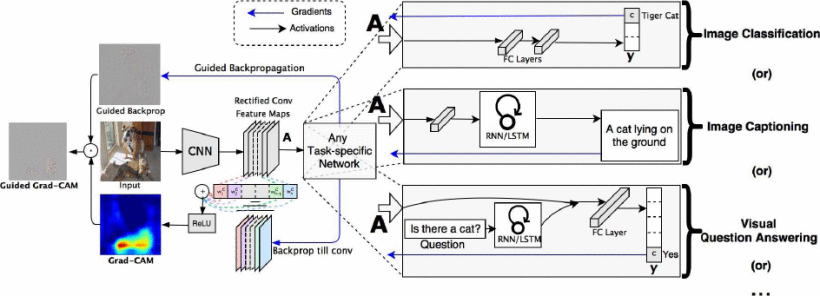
\includegraphics[width=0.9\textwidth]{images/Guided Grad-Cam/large_Guided_GradCam.png}
            \caption{Overview di Guided Grad CAM \cite{selvaraju2017grad}}
            \label{fig:GuidedGCam}
        \end{figure}
        
\subsection{Validazione}
I geni principali sono stati selezionati in base alla classifica dei significance score nelle heatmap. Abbiamo 
applicato l'analisi funzionale a questi top gene per dimostrare ulteriormente che i geni sono specifici per il tumore 
e che sono potenziali biomarker. 
Nella prima fase, abbiamo scelto i primi 400 geni più importanti di ciascun tipo di tumore per effettuare la pathway
analysis (analisi dei percorsi biologici), cercando di scoprire se i percorsi significativamente arricchiti
(significantly enriched pathway) sono correlati al tumore corrispondente. 

\subsubsection{Enchriment Pathway Analysis}~\newline
La Pathway Analysis (PA), nota anche come analisi di arricchimento funzionale, sta rapidamente diventando uno degli
strumenti più importanti della ricerca Omics\footnote{Con il termine OMICS si intendono tutte quelle scienze biologiche
il cui nome termina con il suffisso -omics, ad esempio genomics, transcriptomics, proteomics, metabolomics.}. 
Lo scopo principale degli strumenti di PA è di analizzare i dati ottenuti dalle tecnologie ad alta-capacità di
lavorazione, individuare i gruppi relativi ai geni legati alle alterazioni nei campioni di caso rispetto ad un 
campione di controllo. In questo modo, i metodi di PA cercano di superare il problema della dimensionalità 
introdotta dal dover interpretare grandi liste contenenti geni importanti, ma isolati dal contesto biologico, che
sono l'output principale dell'analisi dei dati ad alta-capacità di lavorazione prodotti dalla maggior parte delle
tecniche biologiche che si basano sull'analisi funzionale, come l'analisi di espressione differenziale. 
I metodi PA invece forniscono significato ai dati biologici sperimentali ad alto rendimento (High Troughput Biological
Data, in breve HTBD) facilitando così l'interpretazione e la successiva generazione di ipotesi. 
Ciò è stato ottenuto sulla base dell'accoppiamento delle conoscenze biologiche esistenti provenienti da banche dati 
con test statistici, analisi matematiche e algoritmi computazionali. I metodi di PA possiedono una vasta gamma 
di applicazioni nella ricerca fisiologica e biomedica. Questi metodi mirano ad aiutare il ricercatore a scoprire 
quali temi biologici, e quali biomolecole, sono cruciali per comprendere i fenomeni in studio, dato gli HTBD
analizzati. A sua volta, gli indizi che fornisce una PA consentono al ricercatore di generare nuove ipotesi, progettare
esperimenti successivi e convalidare ulteriormente i loro risultati. I metodi di PA hanno aiutato i ricercatori
nell'identificazione dei ruoli biologici dei geni candidati, selezionati per progettare nuove terapie per il cancro,
aggirando i danni collaterali alle cellule sane \cite{folger2011predicting}.
Ci sono diversi elementi necessari per eseguire una PA. Prima di tutto, sono necessari dati quantitativi rappresentativi
della biologia cellulare che sono generati con l'uso delle tecnologie di Omics come: RNA-microarrays, tandem mass
spectrometry e RNA-sequencing. 
In secondo luogo, un approccio in grado di analizzare una tale quantità sostanziale di dati è obbligatorio. 
La biologia dei sistemi è un campo di ricerca emergente che consente lo studio degli organismi viventi come sistemi,
opponendosi ad approcci riduzionisti \cite{hartwell1999murray, kitano2002computational}, utilizzando i dati Omics 
come input principale delle sue analisi. In terzo luogo, le conoscenze biologiche molecolari memorizzate in basi 
di dati sono necessarie per l'analisi da eseguire, guidando i metodi PA per cercare le relazioni tra i dati 
Omics generati e temi biologici noti. Infine, il potere computazionale necessario per realizzare PA consiste
principalmente nella computazione necessaria ad eseguire il test statistico dei temi biologici vs. i dati, e 
alla complessità degli altri algoritmi matematici che cercano di estrarre le relazioni tra i dati e le conoscenze
precedenti. 
Un altro esempio è la determinazione della somiglianza e della diversità, a livello molecolare, tra gruppi di campioni,
come nel confronto tra linee cellulari e campioni tumorali \cite{heiser2012subtype}. Questo tipo di analisi può 
aiutare i ricercatori a comprendere i fenomeni di eterogeneità in diversi contesti di ricerca. Un altro esempio 
ancora è l'uso di metodi PA per esaminare la funzione biologica dei moduli genici. I ricercatori hanno
dovuto convalidare insiemi di geni pensati per essere correlati tra loro, come nell'analisi dei geni che fluttuano 
in risposta alle variazioni naturali, come le stagioni \cite{dopico2015widespread}. Anche se tutte queste 
applicazioni hanno avuto successo in obiettivi specifici, l'uso di metodi di PA può essere ampia e complessa come 
la creatività del loro utente. Gli sforzi nella strutturazione della conoscenza biologica sulle pathway hanno provocato 
la generazione delle basi di dati delle pathway (PDBs), anche denominate "basi di conoscenza," che condensano la
conoscenza biologica corrente delle interazioni molecolari nelle raccolte di dati delle pathway. I PDBs di 
solito recuperano e strutturano dati da fonti diverse. Generalmente, le prove sperimentali sono curate dalla 
letteratura e le analisi computazionali sono effettuate dal progetto stesso per inferire le funzioni possibili delle
biomolecole omologhe.
Inoltre, viene generalmente fatto un riferimento incrociato dei dati tra database simili. Ad esempio, le annotazioni 
del database Reactome \cite{vastrik2007reactome} sono curate manualmente dalla letteratura da biologi esperti in
collaborazione con il loro staff editoriale, e cross-referenced con diverse altre risorse, come letteratura primaria,
e altri PDBs correlati \cite{ogata1999kegg}. Aggiunte e correzioni ai PDBs sono effettuate
periodicamente, aumentando così la qualità e la copertura delle loro conoscenze biologiche.
Alcuni database sono in grado di aggiornare le proprie informazioni in modo frequente, per mantenere il passo con le
nuove scoperte. Ad esempio il database KEGG \cite{kanehisa1997database} aggiorna i suoi dati su base settimanale, ma
altri PDBs lo fanno meno spesso, come Gene Ontology \cite{dolinski2000gene}, che aggiorna i suoi dati su base mensile.
Tuttavia, alcuni PDBs non riescono ad aggiornare le loro informazioni in modo regolare, quindi diventano
obsoleti nel corso del tempo, eppure vengono utilizzati dagli utenti di strumenti di PA, quindi si suggerisce 
cautela nell'uso di dati PDB obsoleti.
Quando si esegue la PA è necessario considerare la qualità dei dati nei PDBs e, come ulteriore fattore, è necessario
considerare anche la copertura offerta dai PDBs.
Si tratta della proporzione di componenti biologici aggregati descritti in tutti i percorsi di un PDB rispetto a 
un elenco di riferimento di componenti. 
Ad esempio, uno dei più completi PDB pubblici compositi, Pathway Commons \cite{cerami2010pathway}, con le informazioni
aggregate di 22 PDBs, ha attualmente una copertura di 17.439 simboli genici sui 39.241 accettati, pari a circa 
il $45\%$ dei simboli totali dei registri ufficiali del Comitato per la nomenclatura del genoma HUGO\footnote{
Progetto approvato dal Comitato per la nomenclatura del genoma (HGNC)}. L'utilizzo delle informazioni più aggiornate 
e complete è importante per l'estrazione ottimale di informazioni dai dati sperimentali. Raggiungere questo obiettivo
non è solo un invito agli utenti a utilizzare i migliori PDB disponibili, ma è anche un invito ai
potenziali contributori a migliorare la copertura e la conoscenza contenuta nei database. La maggior parte delle 
banche dati pubbliche incoraggia sforzi di collaborazione aperti, con la corrispondente revisione dei dati condivisi.
Tutti questi miglioramenti nei PDBs porteranno, in conclusione, ad una più rapida scoperta della conoscenza e
ad una più rapida applicazione delle conoscenze biologiche. 
    % 4
    % Sezione 4
\section{Risultati Sperimentali}
\label{sec:result}
Nella seguente sezione mostriamo i risultati ottenuti dalle nostre sperimentazioni e le
comparazioni con il modello di riferimento in \cite{lyu2018deep}.
% 4.1
\subsection{Valutazione Classificazione}
Usando la 10-fold cross validation, è stata calcolata la media totale dell'accuracy, la media dell'accuracy per ogni
classe, la media del precision score $P$, la media del recall score $R$ e la media dell'f1 score $F1$.
\begin{equation}
   P = \frac{TP}{TP + FP}, \quad R = \frac{TP}{TP + FN}, \quad F1 = \frac{2PR}{P + R} 
\end{equation}
Nei paragrafi successivi mostriamo i risultati ottenuti per i test condotti.

% 4.1.1
\subsubsection{Caso Binario}
Per il caso binario, è stato necessario modificare la soglia di varianza utilizzata nella fase di preprocessing
al fine di estrarre un numero di feature (i geni) che fosse più o meno congruo a quello individuato da
\cite{lyu2018deep} in modo da non dover modificare la dimensione delle immagini e da ottenere in maniera più precisa
possibile i potenziali biomarker. 
La soglia utilizzata in questo caso è stata di $0.9552$ e ci ha permesso di avere $10381$ geni.
Le performance ottenute da questo test sono riportate in Tabella \ref{tab:binary_score} a pagina
\pageref{tab:binary_score} mentre l'accuracy divisa per coorte tumorale è riportata in Tabella \ref{tab:bin_test_res}
a pagina \pageref{tab:bin_test_res}. Per completezza, abbiamo generato anche la matrice di confusione riportata in
Figura \ref{fig:cnf_matrix_binary} dalla quale si evince che non ci sono stati errori di classificazione.
% Tabella: [Caso Binario] Performance
\begin{table}[htbp!]
    \centering
    \caption{Performance del caso binario}
    \begin{tabular}{crrrr}
        \toprule
         Metodo & Accuracy & Precision & Recall & F1-score \\
         \midrule
         CNN    & 100\%    & 100\%     & 100\%  & 100\%     \\
         \bottomrule
    \end{tabular}
    \label{tab:binary_score}
\end{table}

% Tabella: [Caso Binario] Accuracy per coorte tumorale
\begin{table}[htbp!]
    \centering 
    \caption{Risultati del caso binario per coorte tumorale}
    %\large{
    \begin{tabular}{llrrr}
    \toprule
    Classe   & Coorte & Numero   & Accuratezza & Accuratezza \\
    tumorale &        & Campioni & ns. metodo  & Riferimento \\
    \midrule
    Lymphoid Neoplasm Diffuse Large B-cell Lymphoma & DLBC & $48$   & 1.00 & 1.00 \\
    Uterine Carcinosarcoma                          & UCS  & $57$   & 1.00 & 0.81 \\ 
    \midrule
    \textbf{Totale campioni}                        &      & $\mathbf{105}$  \\
    \bottomrule
    \label{tab:bin_test_res}
    \end{tabular} 
    %}
\end{table}

% Figura: [Caso Binario] Matrice di Confusione
\begin{figure}
    \centering
    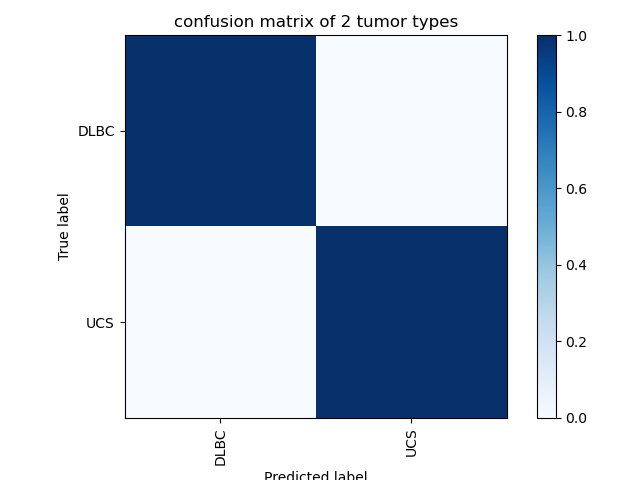
\includegraphics[width=0.7\textwidth]{images/cnfMatrices/cnf_matrix_caso_binario.png}
    \caption{La matrice di confusione del caso binario}
    \label{fig:cnf_matrix_binary}
\end{figure}

% 4.1.2
\subsubsection{Caso Ternario}
Come per il caso binario, anche per il caso ternario è stato necessario modificare la soglia di varianza utilizzata
nella fase di preprocessing per l'estrazione delle feature (i geni). La soglia utilizzata in questo caso è stata di
$0.9869$ e ci ha permesso di avere $10382$ geni. Le performance ottenute in questo test sono riportate in Tabella
\ref{tab:ternary_score} a pagina \pageref{tab:ternary_score} mentre l'accuracy divisa
per coorte tumorale è riportata in Tabella \ref{tab:tern_test_res} a pagina \pageref{tab:tern_test_res}. 
Per completezza, abbiamo generato anche la matrice di confusione riportata in Figura \ref{fig:cnf_matrix_ternary} 
dalla quale si evince che BLCA è stata identificata al 97.56\% correttamente e solo nel 2.44\% è stata 
identificata come CESC; CESC è stata sempre identificata correttamente; LGG è stata identificata correttamente al
98.04\% mentre è stata identificata all'1.96\% come BLCA. 

% Tabella: [Caso Ternario] Performance
\begin{table}[h!]
    \centering
    \caption{Performance del caso ternario}
    \begin{tabular}{crrrr}
        \toprule
         Metodo & Accuracy & Precision & Recall & F1-score \\
         \midrule
         CNN    & 98.37\%    & 98.45\%     & 98.37\%  & 98.37\%     \\
         \bottomrule
    \end{tabular}
    \label{tab:ternary_score}
\end{table}
% Tabella: [Caso Ternario] Accuracy per coorte tumorale
\begin{table}[htbp!]
    \centering 
    \caption{Risultati del caso ternario per coorte tumorale}
    %\large{
    \begin{tabular}{llrrrr}
    \toprule
    Classe   & Coorte & Numero   & Accuratezza & Accuratezza & Accuratezza \\
    tumorale &        & Campioni & ns. metodo  & Variante    & Riferimento \\
    \midrule
    Bladder urothelial carcinoma                    & BLCA & $408$  & 0.98 & & 0.97 \\
    Cervical and endocervical cancers               & CESC & $304$  & 1.00 & & 0.93 \\
    Brain Lower Grade Glioma                        & LGG  & $516$  & 0.98 & & 0.98 \\  
    \midrule
    \textbf{Totale campioni}                        &      & $\mathbf{1.228}$  \\
    \bottomrule
    \label{tab:tern_test_res}
    \end{tabular} 
    %}
\end{table}
% Figura: [Caso Ternario] Matrice di Confusione
\begin{figure}
    \centering
    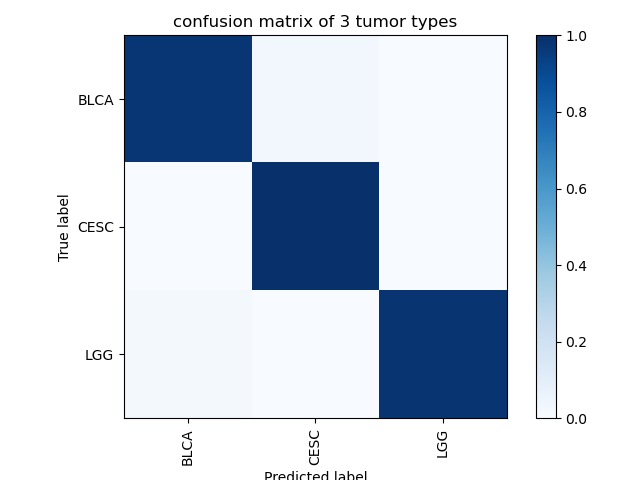
\includegraphics[width=0.7\textwidth]{images/cnfMatrices/cnf_matrix_caso_ternario.png}
    \caption{La matrice di confusione del caso ternario}
    \label{fig:cnf_matrix_ternary}
\end{figure}

% 4.1.3
\subsubsection{Caso Generale}
Le performance ottenute nel test generale usando la rete neurale di \cite{lyu2018deep} sono riportati nella 
Tabella \ref{tab:method_score} a pagina \pageref{tab:method_score} mentre una comparazione dell'accuracy per ogni
classe tumorale è mostrata in Tabella \ref{tab:GPU-res} a pagina \pageref{tab:GPU-res}.
Inoltre, abbiamo anche generato la matrice di confusione così come mostrato in Figura \ref{fig:cnf_matrix_general}.
Dalla matrice di confusione si può notare che la maggior parte delle classi sono classificate correttamente, 
tuttavia ci sono alcune classificazioni errate: 
\begin{enumerate}
    \item i campioni READ sono per lo più sono classificati come COAD e ciò potrebbe essere dovuto alla
          vicinanza delle locazioni spaziali dei due tumori; 
    \item alcuni campioni di CHOL sono classificati erroneamente come LIHC a causa dei pochi campioni presenti per 
          la classe CHOL;
    \item alcuni campioni di ESCA sono classificati erroneamente come STAD;
    \item alcuni campioni di UCS sono classificati erroneamente come UCEC.
\end{enumerate}
Delle possibili motivazioni per gli errori di classificazione (3) e (4) sono riportate nel paragrafo 
\ref{subsec:class-val-varnet} in quanto si sono riscontrate anche durante l'utilizzo della rete VarNet.
% Tabella: [Caso Generale] Performance
\begin{table}[htbp!]
    \centering
    \caption{Performance del metodo utilizzato}
    \begin{tabular}{crrrr}
        \toprule
         Metodo & Accuracy & Precision & Recall & F1-score \\
         \midrule
         CNN    & 95.79\%    & 95.95\%     & 95.79\%  & 95.57\%     \\
         \bottomrule
    \end{tabular}
    \label{tab:method_score}
\end{table}

% Tabella - [VarNet] Accuracy per coorte tumorale
\begin{table}[h!]
    \centering 
    \caption{Accuracy per coorte tumorale (calcolo effettuato su GPU e su dataset con oversampling).}
    \large{
    \begin{tabular}{lrrr}
    \toprule
     Coorte  & Accuratezza & Accuratezza & Accuratezza \\
             & ns. metodo  & Variante    & Riferimento \\
    \midrule
     ACC  & \textbf{1.00} & \textbf{1.00} & 0.95 \\
     BLCA &  \textbf{0.98} & \textbf{0.98} & 0.97 \\
     BRCA &  \textbf{1.00} &\textbf{ 1.00} & 0.99 \\
     CESC &  \textbf{0.97} & \textbf{0.97} & 0.93 \\
     CHOL &  \textbf{0.60} & \textbf{0.60} & 0.56 \\
     COAD &  \textbf{1.00} & \textbf{0.97} & 0.95 \\
     DLBC &  1.00 & 1.00 & 1.00 \\
     ESCA &  \textcolor{blue}{0.75} & \textbf{0.85} & 0.77 \\
     GBM  &  \textbf{1.00} & \textbf{1.00} & 0.94 \\
     HNSC &  0.98 & \textbf{1.00} & 0.98 \\
     KICH &  \textcolor{blue}{0.67} & \textcolor{blue}{0.44} & 0.87 \\
     KIRC &  \textcolor{blue}{0.87} & \textcolor{blue}{0.87} & 0.95 \\
     KIRP &  \textbf{0.94} & \textbf{0.94} & 0.93 \\
     LAML &  1.00 & 1.00 & 1.00 \\
     LGG  &  0.98 & \textbf{1.00} & 0.98 \\
     LIHC &  \textbf{1.00} & \textbf{1.00} & 0.97 \\
     LUAD &  \textcolor{blue}{0.91} & \textbf{0.97} & 0.95 \\
     LUSC &  \textcolor{blue}{0.89} & \textcolor{blue}{0.89} & 0.91 \\
     MESO &  \textbf{1.00} & \textcolor{blue}{0.89} & 0.94 \\
     OV   &  \textcolor{blue}{0.97} & \textbf{1.00} & 0.99 \\
     PAAD &  \textcolor{blue}{0.95} & \textcolor{blue}{0.95} & 0.97 \\
     PCPG &  1.00 & 1.00 & 1.00 \\
     PRAD &  1.00 & 1.00 & 1.00 \\
     READ &  \textcolor{blue}{\textbf{0.09}} & \textcolor{blue}{\textbf{0.09}} & 0.35 \\ 
     SARC &  \textcolor{blue}{0.92} & \textcolor{blue}{0.85} & 0.97 \\ 
     SKCM &  \textcolor{blue}{0.96} & \textcolor{blue}{0.96} & 0.98 \\ 
     STAD &  \textcolor{blue}{0.93} & \textbf{0.98} & 0.96 \\ 
     TGCT &  \textbf{1.00} & \textbf{1.00} & 0.99 \\ 
     THCA &  1.00 & 1.00 & 1.00 \\ 
     THYM &  \textbf{1.00} & \textcolor{blue}{0.92} & 0.99 \\ 
     UCEC &  \textbf{1.00} & \textcolor{blue}{0.95} & 0.96 \\ 
     UCS  &  \textbf{0.83} & \textcolor{blue}{0.67} & 0.81 \\ 
     UVM  &  \textbf{1.00} & \textbf{1.00} & 0.99 \\ 
    \bottomrule
    \label{tab:GPU-res}
    \end{tabular} 
    } %end large
\end{table}
Dal momento che il nostro metodo, al pari di \cite{lyu2018deep} si prefissava di classificare i tumori
e allo stesso tempo individuare i potenziali biomarker, sono stati mantenuti molti geni nella fase
di preprocessing.

% Figura: [Caso Generale] Matrice di Confusione
\begin{figure}[htbp!]
    \centering
    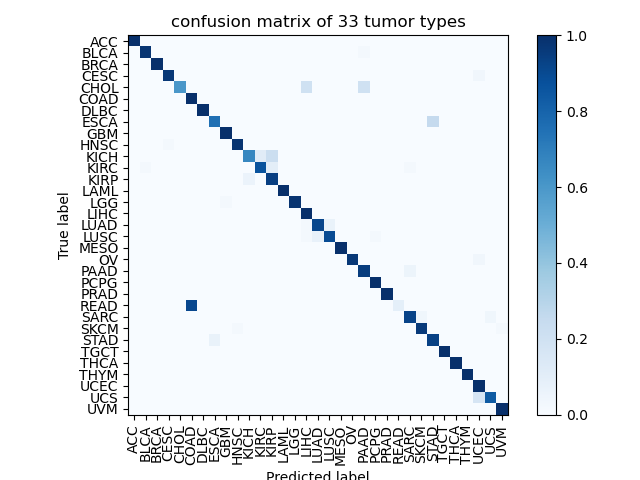
\includegraphics[width=0.7\textwidth]{images/cnfMatrices/cnf_matrix.png}
    \caption{La matrice di confusione del caso generale}
    \label{fig:cnf_matrix_general}
\end{figure}

% 4.2
\subsection{Heat-Map Generate}
\label{subsec:gen_heatmap}
Nelle seguenti sottosezioni saranno mostrati degli esempi di heatmap generate per i vari casi di test effettuati.
Le zone indicate da un contorno \textcolor{red}{rosso} nelle immagini indicano le zone con i pixel più luminosi, ossia
i geni che hanno contribuito maggiormente alla classificazione.

% 4.2.1
\subsubsection{Caso Binario}
Alcuni esempi di heatmap generate nel caso binario sono mostrate nella Figura \ref{fig:bin-heatmap} a pagina 
\pageref{fig:bin-heatmap}.
Si può notare che esiste una certa similarità nelle immagini e in particolare, per DLBC, è possibile
notare lo stesso pattern per le fold 2, 3, 4 e 9.

	\begin{figure}[htpb!]
		\centering
		% prima riga
		\subfloat[][]{
\includegraphics[scale=0.15]{images/bin-heatmaps/DLBCTitle}} \hfill
		\subfloat[][]{\includegraphics[scale=0.7]{images/bin-heatmaps/DLBCFold0}} \hfill % 1
		\subfloat[][]{\includegraphics[scale=0.7]{images/bin-heatmaps/DLBCFold1}} \hfill % 2
		\subfloat[][]{\includegraphics[scale=0.7]{images/bin-heatmaps/DLBCFold2}} \hfill % 3
		\subfloat[][]{\includegraphics[scale=0.7]{images/bin-heatmaps/DLBCFold3}} \hfill % 4
		\subfloat[][]{\includegraphics[scale=0.7]{images/bin-heatmaps/DLBCFold4}} \hfill % 5
		\subfloat[][]{\includegraphics[scale=0.7]{images/bin-heatmaps/DLBCFold5}} \hfill % 6
		\subfloat[][]{\includegraphics[scale=0.7]{images/bin-heatmaps/DLBCFold6}} \hfill % 7
		\subfloat[][]{\includegraphics[scale=0.7]{images/bin-heatmaps/DLBCFold7}} \hfill % 8
		\subfloat[][]{\includegraphics[scale=0.7]{images/bin-heatmaps/DLBCFold8}} \hfill % 9
		\subfloat[][]{\includegraphics[scale=0.7]{images/bin-heatmaps/DLBCFold9}} \\     % 10
	   \vspace{-5mm}
		% seconda riga
		\subfloat[][]{\includegraphics[scale=0.15]{images/bin-heatmaps/UCSTitle}} \hfill
		\subfloat[][]{\includegraphics[scale=0.7]{images/bin-heatmaps/UCSFold0}} \hfill % 11
		\subfloat[][]{\includegraphics[scale=0.7]{images/bin-heatmaps/UCSFold1}} \hfill % 12
		\subfloat[][]{\includegraphics[scale=0.7]{images/bin-heatmaps/UCSFold2}} \hfill % 13
		\subfloat[][]{\includegraphics[scale=0.7]{images/bin-heatmaps/UCSFold3}} \hfill % 14
		\subfloat[][]{\includegraphics[scale=0.7]{images/bin-heatmaps/UCSFold4}} \hfill % 15
		\subfloat[][]{\includegraphics[scale=0.7]{images/bin-heatmaps/UCSFold5}} \hfill % 16
		\subfloat[][]{\includegraphics[scale=0.7]{images/bin-heatmaps/UCSFold6}} \hfill % 17
		\subfloat[][]{\includegraphics[scale=0.7]{images/bin-heatmaps/UCSFold7}} \hfill % 18
		\subfloat[][]{\includegraphics[scale=0.7]{images/bin-heatmaps/UCSFold8}} \hfill % 19
		\subfloat[][]{\includegraphics[scale=0.7]{images/bin-heatmaps/UCSFold9}} \\     % 20
		\caption{Heatmaps del caso binario}
		\label{fig:bin-heatmap}
	\end{figure}

% 4.2.2
\subsubsection{Caso Ternario}
Alcuni esempi di heatmap generate nel caso ternario sono mostrate nella Figura \ref{fig:tern-heatmap} a
pagina \pageref{fig:tern-heatmap}.
Anche in questo caso si può notare che esiste una certa similarità nelle immagini ma purtroppo
non è presente nessun pattern evidente.

	\begin{figure}[htpb!]
		\centering
		% prima riga
		\subfloat[][]{\includegraphics[scale=0.15]{images/tern-heatmaps/BLCATitle}} \hfill
		\subfloat[][]{\includegraphics[scale=0.7]{images/tern-heatmaps/BLCAFold0}} \hfill % 1
		\subfloat[][]{\includegraphics[scale=0.7]{images/tern-heatmaps/BLCAFold1}} \hfill % 2
		\subfloat[][]{\includegraphics[scale=0.7]{images/tern-heatmaps/BLCAFold2}} \hfill % 3
		\subfloat[][]{\includegraphics[scale=0.7]{images/tern-heatmaps/BLCAFold3}} \hfill % 4
		\subfloat[][]{\includegraphics[scale=0.7]{images/tern-heatmaps/BLCAFold4}} \hfill % 5
		\subfloat[][]{\includegraphics[scale=0.7]{images/tern-heatmaps/BLCAFold5}} \hfill % 6
		\subfloat[][]{\includegraphics[scale=0.7]{images/tern-heatmaps/BLCAFold6}} \hfill % 7
		\subfloat[][]{\includegraphics[scale=0.7]{images/tern-heatmaps/BLCAFold7}} \hfill % 8
		\subfloat[][]{\includegraphics[scale=0.7]{images/tern-heatmaps/BLCAFold8}} \hfill % 9
		\subfloat[][]{\includegraphics[scale=0.7]{images/tern-heatmaps/BLCAFold9}} \\     % 10
	   \vspace{-5mm}
		% seconda riga
		\subfloat[][]{\includegraphics[scale=0.15]{images/tern-heatmaps/CESCTitle}} \hfill
		\subfloat[][]{\includegraphics[scale=0.7]{images/tern-heatmaps/CESCFold0}} \hfill % 11
		\subfloat[][]{\includegraphics[scale=0.7]{images/tern-heatmaps/CESCFold1}} \hfill % 12
		\subfloat[][]{\includegraphics[scale=0.7]{images/tern-heatmaps/CESCFold2}} \hfill % 13
		\subfloat[][]{\includegraphics[scale=0.7]{images/tern-heatmaps/CESCFold3}} \hfill % 14
		\subfloat[][]{\includegraphics[scale=0.7]{images/tern-heatmaps/CESCFold4}} \hfill % 15
		\subfloat[][]{\includegraphics[scale=0.7]{images/tern-heatmaps/CESCFold5}} \hfill % 16
		\subfloat[][]{\includegraphics[scale=0.7]{images/tern-heatmaps/CESCFold6}} \hfill % 17
		\subfloat[][]{\includegraphics[scale=0.7]{images/tern-heatmaps/CESCFold7}} \hfill % 18
		\subfloat[][]{\includegraphics[scale=0.7]{images/tern-heatmaps/CESCFold8}} \hfill % 19
		\subfloat[][]{\includegraphics[scale=0.7]{images/tern-heatmaps/CESCFold9}} \\     % 20
		\vspace{-5mm}
			% terza riga
		\subfloat[][]{\includegraphics[scale=0.15]{images/tern-heatmaps/LGGTitle}} \hfill
		\subfloat[][]{\includegraphics[scale=0.7]{images/tern-heatmaps/LGGFold0}} \hfill % 21
		\subfloat[][]{\includegraphics[scale=0.7]{images/tern-heatmaps/LGGFold1}} \hfill % 22
		\subfloat[][]{\includegraphics[scale=0.7]{images/tern-heatmaps/LGGFold2}} \hfill % 23
		\subfloat[][]{\includegraphics[scale=0.7]{images/tern-heatmaps/LGGFold3}} \hfill % 24
		\subfloat[][]{\includegraphics[scale=0.7]{images/tern-heatmaps/LGGFold4}} \hfill % 25
		\subfloat[][]{\includegraphics[scale=0.7]{images/tern-heatmaps/LGGFold5}} \hfill % 26
		\subfloat[][]{\includegraphics[scale=0.7]{images/tern-heatmaps/LGGFold6}} \hfill % 27
		\subfloat[][]{\includegraphics[scale=0.7]{images/tern-heatmaps/LGGFold7}} \hfill % 28
		\subfloat[][]{\includegraphics[scale=0.7]{images/tern-heatmaps/LGGFold8}} \hfill % 29
		\subfloat[][]{\includegraphics[scale=0.7]{images/tern-heatmaps/LGGFold9}} \\     % 30
		\caption{Heatmaps del caso ternario}
		\label{fig:tern-heatmap}
	\end{figure}

% 4.2.3
\subsubsection{Caso Generale}
Le heatmap generate per ogni classe mostrano una similarità tra le 10 fold e mostrano un pattern distinto
quando comparate tra classi. Alcuni esempi sono mostrati nella Figura \ref{fig:esempi-heatmap} a
pagina \pageref{fig:esempi-heatmap}. 
Nell'esempio, ogni riga rappresenta le heatmap di diverse fold (da sinistra a destra sono dalla fold 1 alla fold 10).
Anche se ci sono alcune differenze tra le diverse fold, esiste un pattern chiaro tra di esse.
\begin{figure}[htpb!]
    \centering
    % prima riga
    \subfloat[][]{\includegraphics[scale=0.3]{images/coloredHeatmapsNet/BLCAtitle}} \hfill
    \subfloat[][]{\includegraphics[scale=0.3]{images/coloredHeatmapsNet/BLCAAvgGuidedGcamNormFold0marked}} \hfill % 1
    \subfloat[][]{\includegraphics[scale=0.3]{images/coloredHeatmapsNet/BLCAAvgGuidedGcamNormFold1marked}} \hfill % 2
    \subfloat[][]{\includegraphics[scale=0.3]{images/coloredHeatmapsNet/BLCAAvgGuidedGcamNormFold2marked}} \hfill % 3
    \subfloat[][]{\includegraphics[scale=0.3]{images/coloredHeatmapsNet/BLCAAvgGuidedGcamNormFold3marked}} \hfill % 4
    \subfloat[][]{\includegraphics[scale=0.3]{images/coloredHeatmapsNet/BLCAAvgGuidedGcamNormFold4marked}} \hfill % 5
    \subfloat[][]{\includegraphics[scale=0.3]{images/coloredHeatmapsNet/BLCAAvgGuidedGcamNormFold5marked}} \hfill % 6
    \subfloat[][]{\includegraphics[scale=0.3]{images/coloredHeatmapsNet/BLCAAvgGuidedGcamNormFold6marked}} \hfill % 7
    \subfloat[][]{\includegraphics[scale=0.3]{images/coloredHeatmapsNet/BLCAAvgGuidedGcamNormFold7marked}} \hfill % 8
    \subfloat[][]{\includegraphics[scale=0.3]{images/coloredHeatmapsNet/BLCAAvgGuidedGcamNormFold8marked}} \hfill % 9
    \subfloat[][]{\includegraphics[scale=0.3]{images/coloredHeatmapsNet/BLCAAvgGuidedGcamNormFold9marked}} \\     % 10
   \vspace{-5mm}
    % seconda riga
    \subfloat[][]{\includegraphics[scale=0.3]{images/coloredHeatmapsNet/LGGtitle}} \hfill
    \subfloat[][]{\includegraphics[scale=0.3]{images/coloredHeatmapsNet/LGGAvgGuidedGcamNormFold0marked}} \hfill % 11
    \subfloat[][]{\includegraphics[scale=0.3]{images/coloredHeatmapsNet/LGGAvgGuidedGcamNormFold1marked}} \hfill % 12
    \subfloat[][]{\includegraphics[scale=0.3]{images/coloredHeatmapsNet/LGGAvgGuidedGcamNormFold2marked}} \hfill % 13
    \subfloat[][]{\includegraphics[scale=0.3]{images/coloredHeatmapsNet/LGGAvgGuidedGcamNormFold3marked}} \hfill % 14
    \subfloat[][]{\includegraphics[scale=0.3]{images/coloredHeatmapsNet/LGGAvgGuidedGcamNormFold4marked}} \hfill % 15
    \subfloat[][]{\includegraphics[scale=0.3]{images/coloredHeatmapsNet/LGGAvgGuidedGcamNormFold5marked}} \hfill % 16
    \subfloat[][]{\includegraphics[scale=0.3]{images/coloredHeatmapsNet/LGGAvgGuidedGcamNormFold6marked}} \hfill % 17
    \subfloat[][]{\includegraphics[scale=0.3]{images/coloredHeatmapsNet/LGGAvgGuidedGcamNormFold7marked}} \hfill % 18
    \subfloat[][]{\includegraphics[scale=0.3]{images/coloredHeatmapsNet/LGGAvgGuidedGcamNormFold8marked}} \hfill % 19
    \subfloat[][]{\includegraphics[scale=0.3]{images/coloredHeatmapsNet/LGGAvgGuidedGcamNormFold9marked}} \\     % 20
    \vspace{-5mm}
    % terza riga
    \subfloat[][]{\includegraphics[scale=0.3]{images/coloredHeatmapsNet/PRADtitle}} \hfill
    \subfloat[][]{\includegraphics[scale=0.3]{images/coloredHeatmapsNet/PRADAvgGuidedGcamNormFold0marked}} \hfill % 21
    \subfloat[][]{\includegraphics[scale=0.3]{images/coloredHeatmapsNet/PRADAvgGuidedGcamNormFold1marked}} \hfill % 22
    \subfloat[][]{\includegraphics[scale=0.3]{images/coloredHeatmapsNet/PRADAvgGuidedGcamNormFold2marked}} \hfill % 23
    \subfloat[][]{\includegraphics[scale=0.3]{images/coloredHeatmapsNet/PRADAvgGuidedGcamNormFold3marked}} \hfill % 24
    \subfloat[][]{\includegraphics[scale=0.3]{images/coloredHeatmapsNet/PRADAvgGuidedGcamNormFold4marked}} \hfill % 25
    \subfloat[][]{\includegraphics[scale=0.3]{images/coloredHeatmapsNet/PRADAvgGuidedGcamNormFold5marked}} \hfill % 26
    \subfloat[][]{\includegraphics[scale=0.3]{images/coloredHeatmapsNet/PRADAvgGuidedGcamNormFold6marked}} \hfill % 27
    \subfloat[][]{\includegraphics[scale=0.3]{images/coloredHeatmapsNet/PRADAvgGuidedGcamNormFold7marked}} \hfill % 28
    \subfloat[][]{\includegraphics[scale=0.3]{images/coloredHeatmapsNet/PRADAvgGuidedGcamNormFold8marked}} \hfill % 29
    \subfloat[][]{\includegraphics[scale=0.3]{images/coloredHeatmapsNet/PRADAvgGuidedGcamNormFold9marked}} \hfill % 30
    \caption{Alcuni esempi di heatmap. Ogni colonna rappresenta il risultato di una fold. Nella prima riga ci sono le heatmap %
                del tipo di tumore BLCA, nella seconda di LGG e nella terza di PRAD.}
    \label{fig:esempi-heatmap}
\end{figure}

% 4.3
\subsection{Validazione dei percorsi biologici dei top genes}
\label{ssec:val-bio-net}
Come si può notare dalla Figura \ref{fig:confidence-score-Net} a pagina \pageref{fig:confidence-score-Net}, 
l'intensità dei primi 100 geni decresce rapidamente, mentre l'intensità dei geni successivi decresce in maniera 
uniforme. Tale comportamento è stato constatato anche in \cite{lyu2018deep}. Inoltre, quando
l'intensità è bassa, il tasso di decrescita cresce di nuovo. Se, come hanno fatto in \cite{lyu2018deep}, si assume 
che un'intensità più alta implica una \textit{significance} più alta, dal momento che la curva delle intensità nei
primi 400 geni cambia in maniera più evidente (ossia è più grande) rispetto alle altra migliaia di geni, allora 
è lecito scegliere i primi 400 geni come query per effettuare la pathway analysis. In aggiunta, facendo una
comparazione con il numero totale di geni considerati (10381), la scelta di 400 geni è 
consistente col fatto che il numero di biomarker dovrebbe essere basso. Per effettuare la KEGG\footnote{Kyoto
Encyclopedia of Genes and Genomes} pathway analysis è stato utilizzato il tool
DAVID\footnote{\url{https://david.ncifcrf.gov/home.jsp}}.
In seguito, basandoci sui risultati già ottenuti da \cite{lyu2018deep} e facendo una sommaria attività di 
literature review, limitata alla nostra conoscenza attuale, abbiamo provato a trovare le relazioni che sussistono 
tra le pathway individuate e i tipi di tumore. Le pathway individuate, con un P-value inferiore a $10^{-3}$, per 
i casi di test effettuati, sono mostrate nelle successive sezioni.
% Figura - Confidence score
\begin{figure}
    \centering
    \includegraphics[width=0.7\textwidth]{images/confidence-score/ConfidenceScore-plot-Net.png}
    \caption{I cambi di intensità nelle heatmap per ogni classe. Si può notare come alcune classi condividano lo stesso pattern nei
    cambi di intensità.}
    \label{fig:confidence-score-Net}
\end{figure}
Nelle Tabelle che seguiranno si utilizzerà la seguente legenda: i valori di questo \textcolor{\clrnew}{colore} 
sono le nuove pathway rilevate dalle nostre analisi con il tool DAVID, i valori con questo 
\colorbox{\clrmatch}{background} indicano le path che trovano riscontro anche nel lavoro di Lyu e Haque
\cite{lyu2018deep} e i valori con questo \colorbox{\clrpath}{\textbf{background}} indicano quelle pathway che 
sono specifiche della coorte tumorale.
\subsubsection{Caso Binario}~\newline
Come si può notare dalla Tabella che segue, le pathway ottenute in questo caso binario, a differenza delle
stesse classi tumorali riportate nella sezione \ref{ssec:val-bio-net}, sono molte di più e, a differenza
di quanto rilevato in \cite{lyu2018deep} nel 2018, sono presenti anche malattie di origini recente (ad es. il Corona
Virus).
Per UCS inoltre, si può notare che sono presenti quattro pathway tumorali note: Wnt signaling pathway, PI3K-Akt
signaling pathway, Hippo signaling pathway e TGF-beta signaling pathway, tre delle quali (Wnt, Hippo e TGF-beta)
scompaiono nel caso generale descritto nella sezione \ref{ssec:val-bio-net}.

Tali risultati sono ottenuti in quanto il numero di classi in esame è molto piccolo e dunque, al momento della
classificazione, non viene sfruttata la conoscenza di ulteriori classi tumorali e in sede di generazione delle heatmap, 
e quindi di attribuzione del significance score ai geni (dal momento che si scopre quali geni hanno contribuito di più 
alla classificazione), il valore che viene assegnato ai geni è diverso e quindi ne consegue che anche la selezione 
dei top 400 effettuata in questo caso è diversa rispetto al caso generale.
\begin{longtable}{cllr}
%intestazione iniziale
\caption{Risultati della Pathways Analysis sui primi 400 geni per le coorti DLBC e UCS ($P < 10^{-3}$)} \\
\toprule
\multirow{2}{*}{Tumore} & \multicolumn{2}{l}{Pathway correlata} & \multirow{2}{*}{P value} \\
& ID & Nome \\
\midrule
\endfirsthead
\toprule
\multirow{2}{*}{Tumore} & \multicolumn{2}{l}{Pathway correlata} & \multirow{2}{*}{P value} \\
& ID & Nome \\
\midrule
\endhead
\midrule
\multicolumn{2}{r}{Continua nella prossima pagina}
\endfoot
\bottomrule
\endlastfoot
DLBC & hsa05169 & \textcolor{\clrnew}{Epstein-Barr virus infection} & 1.43e-16\\ 
 \rowcolor{\clrmatch} & hsa05166 & Human T-cell leukemia virus 1 infection & 1.01e-13 \\ 
 & hsa04659 & \textcolor{\clrnew}{Th17 cell differentiation} & 1.28e-13 \\ 
 & hsa04658 & \textcolor{\clrnew}{Th1 and Th2 cell differentiation} & 3.13e-13 \\ 
 \rowcolor{\clrpath} & hsa04062 & \textbf{Chemokine signaling pathway} & 3.10e-12 \\ 
 \rowcolor{\clrpath} & hsa05330 & \textbf{Allograft rejection} & 9.20e-12 \\ 
 \rowcolor{\clrmatch} & hsa04612 & Antigen processing and presentation & 5.07e-11 \\ 
 \rowcolor{\clrmatch} & hsa05140 & Leishmaniasis & 1.94e-10 \\ 
 \rowcolor{\clrmatch}& hsa04940 & Type I diabetes mellitus & 2.02e-10 \\ 
 \rowcolor{\clrpath} & hsa05332 & \textbf{Graft-versus-host disease} & 9.73e-10 \\ 
 \rowcolor{\clrmatch} & hsa05145 & Toxoplasmosis & 1.02e-09 \\ 
 \rowcolor{\clrmatch} & hsa05416 & Viral myocarditis & 1.72e-09 \\ 
 \rowcolor{\clrpath} & hsa04064 & \textbf{NF-kappa B signaling pathway} & 1.98e-09 \\ 
 \rowcolor{\clrmatch} & hsa05321 & Inflammatory bowel disease & 2.09e-09 \\ 
 & hsa04380 & \textcolor{\clrnew}{Osteoclast differentiation} & 3.82e-09 \\ 
 & hsa04668 & \textcolor{\clrnew}{TNF signaling pathway} & 4.10e-09 \\ 
 & hsa05340 & \textcolor{\clrnew}{Primary immunodeficiency} & 7.56e-09 \\ 
 & hsa04061 & \textcolor{\clrnew}{Viral protein interaction with cytokine and cytokine receptor} & 4.56e-08 \\ 
 & hsa05200 & \textcolor{\clrnew}{Pathways in cancer} & 8.57e-08 \\ 
 \rowcolor{\clrmatch} & hsa05323 & Rheumatoid arthritis & 1.18e-07 \\ 
 & hsa05163 & \textcolor{\clrnew}{Human cytomegalovirus infection} & 1.19e-07 \\ 
 \rowcolor{\clrmatch} & hsa05320 & Autoimmune thyroid disease & 1.26e-07 \\ 
 \rowcolor{\clrmatch} & hsa04672 & Intestinal immune network for IgA production & 1.57e-07 \\ 
 \rowcolor{\clrmatch} & hsa05150 & Staphylococcus aureus infection & 2.47e-07 \\ 
 & hsa05167 & \textcolor{\clrnew}{Kaposi sarcoma-associated herpesvirus infection} & 3.78e-07 \\ 
 \rowcolor{\clrpath} & hsa04514 & \textbf{Cell adhesion molecules} & 4.20e-07 \\ 
 \rowcolor{\clrpath} & hsa04662 & \textbf{B cell receptor signaling pathway} & 4.29e-07 \\ 
 \rowcolor{\clrmatch} & hsa04060 & Cytokine-cytokine receptor interaction & 4.36e-07 \\ 
 & hsa05417 & \textcolor{\clrnew}{Lipid and atherosclerosis} & 4.78e-07 \\ 
 \rowcolor{\clrmatch} & hsa04640 & Hematopoietic cell lineage & 4.99e-07 \\ 
 \rowcolor{\clrmatch} & hsa05310 & Asthma & 7.56e-07 \\ 
 \rowcolor{\clrmatch} & hsa05152 & Tuberculosis & 8.38e-07 \\ 
 \rowcolor{\clrmatch} & hsa04145 & Phagosome & 1.48e-06 \\ 
 & hsa04933 & \textcolor{\clrnew}{AGE-RAGE signaling pathway in diabetic complications} & 2.16e-06 \\ 
 & hsa05130 & \textcolor{\clrnew}{Pathogenic Escherichia coli infection} & 3.86e-06 \\ 
 & hsa05170 & \textcolor{\clrnew}{Human immunodeficiency virus 1 infection} & 4.80e-06 \\ 
 & hsa04210 & \textcolor{\clrnew}{Apoptosis} & 6.52e-06 \\ 
 & hsa05171 & \textcolor{\clrnew}{Coronavirus disease - COVID-19} & 1.05e-05 \\ 
 & hsa05162 & \textcolor{\clrnew}{Measles} & 1.06e-05 \\ 
 & hsa05205 & \textcolor{\clrnew}{Proteoglycans in cancer} & 1.10e-05 \\ 
 & hsa04611 & \textcolor{\clrnew}{Platelet activation} & 1.98e-05 \\ 
 & hsa05418 & \textcolor{\clrnew}{Fluid shear stress and atherosclerosis} & 2.83e-05 \\ 
 & hsa04670 & \textcolor{\clrnew}{Leukocyte transendothelial migration} & 3.00e-05 \\ 
 & hsa05142 & \textcolor{\clrnew}{Chagas disease} & 3.17e-05 \\ 
 & hsa04926 & \textcolor{\clrnew}{Relaxin signaling pathway} & 4.36e-05 \\ 
 & hsa04015 & \textcolor{\clrnew}{Rap1 signaling pathway} & 4.60e-05 \\ 
 & hsa05164 & \textcolor{\clrnew}{Influenza A} & 6.03e-05 \\ 
 & hsa05215 & \textcolor{\clrnew}{Prostate cancer} & 1.12e-04 \\ 
 & hsa04625 & \textcolor{\clrnew}{C-type lectin receptor signaling pathway} & 1.27e-04 \\ 
 & hsa05202 & \textcolor{\clrnew}{Transcriptional misregulation in cancer} & 1.58e-04 \\ 
 & hsa05161 & \textcolor{\clrnew}{Hepatitis B} & 2.46e-04 \\ 
 & hsa04218 & \textcolor{\clrnew}{Cellular senescence} & 2.74e-04 \\ 
 & hsa04010 & \textcolor{\clrnew}{MAPK signaling pathway} & 2.82e-04 \\ 
 & hsa04620 & \textcolor{\clrnew}{Toll-like receptor signaling pathway} & 3.39e-04 \\ 
 & hsa04660 & \textcolor{\clrnew}{T cell receptor signaling pathway} & 3.39e-04 \\ 
 & hsa04610 & \textcolor{\clrnew}{Complement and coagulation cascades} & 4.06e-04 \\ 
 & hsa04928 & \textcolor{\clrnew}{Parathyroid hormone synthesis, secretion and action} & 4.52e-04 \\ 
 & hsa05132 & \textcolor{\clrnew}{Salmonella infection} & 5.33e-04 \\ 
 & hsa05133 & \textcolor{\clrnew}{Pertussis} & 6.18e-04 \\ 
 & hsa05219 & \textcolor{\clrnew}{Bladder cancer} & 6.71e-04 \\ 
 & hsa04151 & \textcolor{\clrnew}{PI3K-Akt signaling pathway} & 8.15e-04 \\ 
 & hsa05203 & \textcolor{\clrnew}{Viral carcinogenesis} & 9.87e-04 \\ 
\midrule 
\rowcolor{\clrmatch} UCS & hsa04512 & ECM-receptor interaction & 1.14e-13\\ 
 & hsa05165 & \textcolor{\clrnew}{Human papillomavirus infection} & 3.44e-12 \\ 
 \rowcolor{\clrmatch}& hsa04510 & Focal adhesion & 1.42e-11 \\ 
 & hsa05200 & \textcolor{\clrnew}{Pathways in cancer} & 3.14e-10 \\ 
 & hsa05205 & \textcolor{\clrnew}{Proteoglycans in cancer} & 9.14e-09 \\ 
 & hsa04360 & \textcolor{\clrnew}{Axon guidance} & 1.11e-08 \\ 
 & hsa04810 & \textcolor{\clrnew}{Regulation of actin cytoskeleton} & 2.26e-08 \\ 
 & hsa04310 & \textcolor{\clrnew}{Wnt signaling pathway} & 9.72e-08 \\ 
 & hsa04151 & \textcolor{\clrnew}{PI3K-Akt signaling pathway} & 1.24e-07 \\ 
 \rowcolor{\clrmatch}& hsa04974 & Protein digestion and absorption & 1.48e-07 \\ 
 & hsa05412 & \textcolor{\clrnew}{Arrhythmogenic right ventricular cardiomyopathy} & 1.61e-07 \\ 
 & hsa04514 & \textcolor{\clrnew}{Cell adhesion molecules} & 5.23e-06 \\ 
 & hsa04390 & \textcolor{\clrnew}{Hippo signaling pathway} & 1.36e-05 \\ 
 & hsa04520 & \textcolor{\clrnew}{Adherens junction} & 3.02e-05 \\ 
 & hsa04670 & \textcolor{\clrnew}{Leukocyte transendothelial migration} & 4.25e-05 \\ 
 & hsa05224 & \textcolor{\clrnew}{Breast cancer} & 5.20e-05 \\ 
 & hsa05217 & \textcolor{\clrnew}{Basal cell carcinoma} & 6.10e-05 \\ 
 & hsa05222 & \textcolor{\clrnew}{Small cell lung cancer} & 6.35e-05 \\ 
 & hsa04530 & \textcolor{\clrnew}{Tight junction} & 7.02e-05 \\ 
 & hsa05410 & \textcolor{\clrnew}{Hypertrophic cardiomyopathy} & 1.30e-04 \\ 
 & hsa04015 & \textcolor{\clrnew}{Rap1 signaling pathway} & 1.54e-04 \\ 
 & hsa04933 & \textcolor{\clrnew}{AGE-RAGE signaling pathway in diabetic complications} & 2.46e-04 \\ 
 & hsa04350 & \textcolor{\clrnew}{TGF-beta signaling pathway} & 3.00e-04 \\ 
 & hsa05166 & \textcolor{\clrnew}{Human T-cell leukemia virus 1 infection} & 5.11e-04 \\ 
 & hsa04928 & \textcolor{\clrnew}{Parathyroid hormone synthesis, secretion and action} & 5.99e-04 \\ 
 & hsa05225 & \textcolor{\clrnew}{Hepatocellular carcinoma} & 6.83e-04 \\ 
 & hsa04270 & \textcolor{\clrnew}{Vascular smooth muscle contraction} & 7.20e-04 \\ 
 & hsa04934 & \textcolor{\clrnew}{Cushing syndrome} & 7.56e-04 \\ 
 & hsa05414 & \textcolor{\clrnew}{Dilated cardiomyopathy} & 9.12e-04 \\ 
\midrule 
\end{longtable} 

\subsubsection{Caso Ternario}~\newline
Anche per il caso ternario, così come accaduto per il binario, se si fa un confronto con quanto riportato nella sezione
\ref{ssec:val-bio-net}, è possibile notare che il numero di pathway rilevate per le stesse classi tumorali è maggiore.
Come già indicato nel caso binario, tali risultati sono dovuti al fatto che sono prese in esame poche classi tumorali
e quindi i significance score dei geni sono diversi rispetto al caso generale.
Non è presente un grande differenza con i risultati del caso generale, per cui vale quanto detto nella 
sezione \ref{ssec:val-bio-net} per le stesse classi tumorali.

\begin{longtable}{cllr}
%intestazione iniziale
\caption{Risultati della Pathways Analysis sui primi 400 geni per le coorti BLCA, CESC e LGG ($P < 10^{-3}$)} \\
\toprule
\multirow{2}{*}{Tumore} & \multicolumn{2}{l}{Pathway correlata} & \multirow{2}{*}{P value} \\
& ID & Nome \\
\midrule
\endfirsthead
\toprule
\multirow{2}{*}{Tumore} & \multicolumn{2}{l}{Pathway correlata} & \multirow{2}{*}{P value} \\
& ID & Nome \\
\midrule
\endhead
\midrule
\multicolumn{2}{r}{Continua nella prossima pagina}
\endfoot
\bottomrule
\endlastfoot
\rowcolor{\clrmatch} BLCA & hsa04512 & ECM-receptor interaction & 4.05e-09\\ 
\rowcolor{\clrmatch}& hsa04510 & Focal adhesion & 8.89e-09 \\ 
 & hsa05205 & \textcolor{\clrnew}{Proteoglycans in cancer} & 1.37e-07 \\ 
 & hsa05204 & \textcolor{\clrnew}{Chemical carcinogenesis - DNA adducts} & 5.87e-07 \\ 
 & hsa04514 & \textcolor{\clrnew}{Cell adhesion molecules} & 6.51e-07 \\ 
 \rowcolor{\clrmatch} & hsa00980 & Metabolism of xenobiotics by cytochrome P450 & 5.81e-06 \\ 
 & hsa04145 & \textcolor{\clrnew}{Phagosome} & 1.69e-05 \\ 
 & hsa00983 & \textcolor{\clrnew}{Drug metabolism - other enzymes} & 3.14e-05 \\ 
 & hsa00982 & \textcolor{\clrnew}{Drug metabolism - cytochrome P450} & 6.86e-05 \\ 
 \rowcolor{\clrpath} & hsa00140 & \textbf{Steroid hormone biosynthesis} & 9.77e-05 \\ 
 & hsa05200 & \textcolor{\clrnew}{Pathways in cancer} & 4.02e-04 \\ 
 & hsa04926 & \textcolor{\clrnew}{Relaxin signaling pathway} & 4.53e-04 \\ 
 & hsa00040 & \textcolor{\clrnew}{Pentose and glucuronate interconversions} & 4.62e-04 \\ 
 & hsa05165 & \textcolor{\clrnew}{Human papillomavirus infection} & 4.64e-04 \\ 
 & hsa04360 & \textcolor{\clrnew}{Axon guidance} & 6.36e-04 \\ 
 & hsa04933 & \textcolor{\clrnew}{AGE-RAGE signaling pathway in diabetic complications} & 8.93e-04 \\ 
\midrule 
CESC & hsa04514 & \textcolor{\clrnew}{Cell adhesion molecules} & 6.07e-10\\ 
 & hsa04512 & \textcolor{\clrnew}{ECM-receptor interaction} & 1.37e-07 \\ 
 & hsa05169 & \textcolor{\clrnew}{Epstein-Barr virus infection} & 1.98e-07 \\ 
 & hsa04612 & \textcolor{\clrnew}{Antigen processing and presentation} & 7.53e-07 \\ 
 & hsa04530 & \textcolor{\clrnew}{Tight junction} & 4.43e-06 \\ 
 & hsa05200 & \textcolor{\clrnew}{Pathways in cancer} & 6.27e-06 \\ 
 & hsa05330 & \textcolor{\clrnew}{Allograft rejection} & 6.41e-06 \\ 
 & hsa04940 & \textcolor{\clrnew}{Type I diabetes mellitus} & 6.57e-06 \\ 
 & hsa05166 & \textcolor{\clrnew}{Human T-cell leukemia virus 1 infection} & 7.30e-06 \\ 
 & hsa04510 & \textcolor{\clrnew}{Focal adhesion} & 7.73e-06 \\ 
 & hsa05416 & \textcolor{\clrnew}{Viral myocarditis} & 9.17e-06 \\ 
 & hsa05150 & \textcolor{\clrnew}{Staphylococcus aureus infection} & 1.07e-05 \\ 
 & hsa05332 & \textcolor{\clrnew}{Graft-versus-host disease} & 2.42e-05 \\ 
 & hsa05146 & \textcolor{\clrnew}{Amoebiasis} & 3.19e-05 \\ 
 & hsa05145 & \textcolor{\clrnew}{Toxoplasmosis} & 5.64e-05 \\ 
 \rowcolor{\clrpath}& hsa05205 & \textbf{Proteoglycans in cancer} & 6.76e-05 \\ 
 & hsa04659 & \textcolor{\clrnew}{Th17 cell differentiation} & 8.51e-05 \\ 
 & hsa04145 & \textcolor{\clrnew}{Phagosome} & 1.22e-04 \\ 
 & hsa04658 & \textcolor{\clrnew}{Th1 and Th2 cell differentiation} & 1.56e-04 \\ 
 & hsa04640 & \textcolor{\clrnew}{Hematopoietic cell lineage} & 1.66e-04 \\ 
 & hsa05323 & \textcolor{\clrnew}{Rheumatoid arthritis} & 1.83e-04 \\ 
 & hsa00330 & \textcolor{\clrnew}{Arginine and proline metabolism} & 2.05e-04 \\ 
 & hsa05133 & \textcolor{\clrnew}{Pertussis} & 2.78e-04 \\ 
 & hsa05140 & \textcolor{\clrnew}{Leishmaniasis} & 3.31e-04 \\ 
 & hsa05418 & \textcolor{\clrnew}{Fluid shear stress and atherosclerosis} & 3.44e-04 \\ 
 & hsa04218 & \textcolor{\clrnew}{Cellular senescence} & 4.56e-04 \\ 
 & hsa04670 & \textcolor{\clrnew}{Leukocyte transendothelial migration} & 5.31e-04 \\ 
 & hsa04657 & \textcolor{\clrnew}{IL-17 signaling pathway} & 5.92e-04 \\ 
 & hsa04810 & \textcolor{\clrnew}{Regulation of actin cytoskeleton} & 6.94e-04 \\ 
\midrule 
\rowcolor{\clrpath}LGG & hsa04010 & \textbf{MAPK signaling pathway **} & 1.26e-08\\ 
 & hsa04724 & \textcolor{\clrnew}{Glutamatergic synapse} & 4.80e-08 \\ 
 & hsa04727 & \textcolor{\clrnew}{GABAergic synapse} & 1.05e-06 \\ 
 & hsa04514 & \textcolor{\clrnew}{Cell adhesion molecules} & 5.96e-06 \\ 
 & hsa04713 & \textcolor{\clrnew}{Circadian entrainment} & 6.16e-06 \\ 
 & hsa04728 & \textcolor{\clrnew}{Dopaminergic synapse} & 1.58e-05 \\ 
 & hsa04360 & \textcolor{\clrnew}{Axon guidance} & 3.27e-05 \\ 
 & hsa05200 & \textcolor{\clrnew}{Pathways in cancer} & 1.04e-04 \\ 
 & hsa04725 & \textcolor{\clrnew}{Cholinergic synapse} & 1.08e-04 \\ 
 & hsa05032 & \textcolor{\clrnew}{Morphine addiction} & 1.69e-04 \\ 
 & hsa04015 & \textcolor{\clrnew}{Rap1 signaling pathway} & 3.59e-04 \\ 
 & hsa04014 & \textcolor{\clrnew}{Ras signaling pathway} & 5.50e-04 \\ 
 & hsa04371 & \textcolor{\clrnew}{Apelin signaling pathway} & 6.37e-04 \\ 
 & hsa05031 & \textcolor{\clrnew}{Amphetamine addiction} & 7.16e-04 \\ 
 & hsa05205 & \textcolor{\clrnew}{Proteoglycans in cancer} & 8.80e-04 \\ 
 & hsa04926 & \textcolor{\clrnew}{Relaxin signaling pathway} & 9.72e-04 \\ 
\midrule 
\end{longtable} 

\subsubsection{Caso Generale}~\newline
\label{sssec:bio-val-net}
Come è possibile notare dalla Tabella che segue, a differenza di \cite{lyu2018deep}, sono state trovate pathway per
tutte le classi tumorali ma solo 17 hanno mostrato almeno una pathway collegata allo specifico tipo 
di tumore. I geni contenuti in tali pathway possono essere considerati biomarker specifici del tumore.
Per le classi rimanenti, che non hanno mostrato pathway specifiche correlate alla coorte, sono state
individuate diverse pathway concorrenti. Ad esempio, per le classi ACC, KICH, LGG, PCPG e UVM
è stata rilevata la MAPK signaling pathway che è una nota pathway tumorale che si occupa della sopravvivenza
delle cellule. Analizzando i geni correlati a questa pathway, si può notare che essi non sono gli stessi
per tutte le classi sopramenzionate e dunque tali geni possono essere considerati candidati biomarker.
Stesso discorso può essere fatto per le classi BRCA, CHOL, ESCA, GBM, KIRP, LUSC, PCPG e SARC, che pur non avendo 
mostrato pathway specifiche hanno mostrato la PI3K-Akt signaling che è una nota pathway tumorale per la
sopravvivenza delle cellule proprio come la MAPK signaling pathway. ESCA, GBM e KICH hanno mostrato anche la Hippo
signaling pathway che si occupa di controllare le dimensioni degli organi regolando la proliferazione cellulare, 
l'apoptosi e l'auto-rinnovamento delle cellule staminali e la cui disregolazione è noto contribuisca allo sviluppo 
dei cancri.   
Un'altra considerazione può essere fatta per ESCA, KICH, KIRP, SARC, SKCM, TGCT, THCA e UCS che hanno mostrato
come pathway correlate ECM-receptor e Focal Adhesion e, anche in questo caso, analizzando i geni
correlati a tali pathway, è possibile notare che essi non coincidono per tutte le classi e quindi sono
dei potenziali biomarker.
Una nota a parte meritano la classi CHOL, KICH e READ che, seppur non sono state omesse dai risultati per completezza, 
la loro valenza è relativa in quanto: READ viene ignorata completamente in quanto l'accuracy ottenuta è troppo bassa 
e CHOL e KICH hanno un numero troppo limitato di campioni.
    
\begin{longtable}{cllr}
%intestazione iniziale
\caption{Risultati della Pathways Analysis sui primi 400 geni per ogni tipo di tumore ($P < 10^{-3}$)} \\
\toprule
\multirow{2}{*}{Tumore} & \multicolumn{2}{l}{Pathway correlata} & \multirow{2}{*}{P value} \\
& ID & Nome \\
\midrule
\endfirsthead
\toprule
\multirow{2}{*}{Tumore} & \multicolumn{2}{l}{Pathway correlata} & \multirow{2}{*}{P value} \\
& ID & Nome \\
\midrule
\endhead
\midrule
\multicolumn{2}{r}{Continua nella prossima pagina}
\endfoot
\bottomrule
\endlastfoot
ACC & hsa04010 & \textcolor{\clrnew}{MAPK signaling pathway} & 2.58e-07\\ 
    & hsa04015 & \textcolor{\clrnew}{Rap1 signaling pathway} & 2.65e-05 \\ 
     & hsa04512 & \textcolor{\clrnew}{ECM-receptor interaction} & 3.77e-05 \\ 
     & hsa04976 & \textcolor{\clrnew}{Bile secretion} & 1.33e-04 \\ 
     & hsa04115 & \textcolor{\clrnew}{p53 signaling pathway} & 3.75e-04 \\ 
     & hsa04610 & \textcolor{\clrnew}{Complement and coagulation cascades} & 5.56e-04 \\ 
     & hsa05144 & \textcolor{\clrnew}{Malaria} & 7.06e-04 \\ 
\midrule 
\rowcolor{\clrmatch}BLCA & hsa04512 & ECM-receptor interaction & 9.98e-08\\ 
 & hsa05205 & \textcolor{\clrnew}{Proteoglycans in cancer} & 2.15e-07 \\ 
 & hsa04514 & \textcolor{\clrnew}{Cell adhesion molecules} & 7.48e-06 \\ 
 \rowcolor{\clrmatch}& hsa04510 & Focal adhesion & 1.01e-05 \\ 
 & hsa05150 & \textcolor{\clrnew}{Staphylococcus aureus infection} & 7.54e-05 \\ 
 & hsa04270 & \textcolor{\clrnew}{Vascular smooth muscle contraction} & 1.26e-04 \\ 
 & hsa04668 & \textcolor{\clrnew}{TNF signaling pathway} & 1.64e-04 \\ 
 & hsa05200 & \textcolor{\clrnew}{Pathways in cancer} & 2.11e-04 \\ 
 & hsa04933 & \textcolor{\clrnew}{AGE-RAGE signaling pathway in diabetic complications} & 4.00e-04 \\ 
 & hsa04913 & \textcolor{\clrnew}{Ovarian steroidogenesis} & 5.06e-04 \\ 
 & hsa05165 & \textcolor{\clrnew}{Human papillomavirus infection} & 9.06e-04 \\ 
 & hsa05166 & \textcolor{\clrnew}{Human T-cell leukemia virus 1 infection} & 9.85e-04 \\ 
\midrule 
BRCA & hsa04915 & \textcolor{\clrnew}{Estrogen signaling pathway} & 2.38e-08\\ 
 \rowcolor{\clrmatch}& hsa04512 & ECM-receptor interaction & 2.44e-08 \\ 
 \rowcolor{\clrpath}& hsa04151 & \textbf{PI3K-Akt signaling pathway *} & 4.61e-06 \\ 
 & hsa04927 & \textcolor{\clrnew}{Cortisol synthesis and secretion} & 8.11e-06 \\ 
 & hsa04928 & \textcolor{\clrnew}{Parathyroid hormone synthesis, secretion and action} & 2.10e-05 \\ 
 & hsa04934 & \textcolor{\clrnew}{Cushing syndrome} & 3.31e-05 \\ 
 \rowcolor{\clrmatch}& hsa04510 & Focal adhesion & 4.96e-05 \\ 
 & hsa05205 & \textcolor{\clrnew}{Proteoglycans in cancer} & 8.05e-05 \\ 
 & hsa05165 & \textcolor{\clrnew}{Human papillomavirus infection} & 8.86e-05 \\ 
 \rowcolor{\clrpath}& hsa03320 & \textbf{PPAR signaling pathway *} & 8.95e-05 \\ 
 & hsa04514 & \textcolor{\clrnew}{Cell adhesion molecules} & 1.03e-04 \\ 
 & hsa04145 & \textcolor{\clrnew}{Phagosome} & 1.20e-04 \\ 
 & hsa04933 & \textcolor{\clrnew}{AGE-RAGE signaling pathway in diabetic complications} & 1.51e-04 \\ 
 & hsa05200 & \textcolor{\clrnew}{Pathways in cancer} & 5.14e-04 \\ 
 & hsa01522 & \textcolor{\clrnew}{Endocrine resistance} & 7.22e-04 \\ 
 & hsa04926 & \textcolor{\clrnew}{Relaxin signaling pathway} & 7.76e-04 \\ 
 & hsa04540 & \textcolor{\clrnew}{Gap junction} & 9.62e-04 \\ 
\midrule 
CESC & hsa05200 & \textcolor{\clrnew}{Pathways in cancer} & 8.37e-07\\ 
 & hsa04115 & \textcolor{\clrnew}{p53 signaling pathway} & 4.64e-06 \\ 
 \rowcolor{\clrpath}& hsa05205 & \textbf{Proteoglycans in cancer} & 5.71e-05 \\ 
 & hsa05222 & \textcolor{\clrnew}{Small cell lung cancer} & 8.00e-05 \\ 
 & hsa04512 & \textcolor{\clrnew}{ECM-receptor interaction} & 1.14e-04 \\ 
 & hsa04110 & \textcolor{\clrnew}{Cell cycle} & 1.54e-04 \\ 
 & hsa05146 & \textcolor{\clrnew}{Amoebiasis} & 1.57e-04 \\ 
 & hsa04080 & \textcolor{\clrnew}{Neuroactive ligand-receptor interaction} & 1.79e-04 \\ 
 & hsa04915 & \textcolor{\clrnew}{Estrogen signaling pathway} & 2.85e-04 \\ 
 & hsa04934 & \textcolor{\clrnew}{Cushing syndrome} & 4.46e-04 \\ 
 & hsa05144 & \textcolor{\clrnew}{Malaria} & 5.78e-04 \\ 
\midrule 
CHOL & hsa04512 & \textcolor{\clrnew}{ECM-receptor interaction} & 3.94e-10\\ 
 & hsa04610 & \textcolor{\clrnew}{Complement and coagulation cascades} & 1.92e-08 \\ 
 & hsa00340 & \textcolor{\clrnew}{Histidine metabolism} & 6.82e-06 \\ 
 & hsa04061 & \textcolor{\clrnew}{Viral protein interaction with cytokine and cytokine receptor} & 8.03e-06 \\ 
 & hsa04514 & \textcolor{\clrnew}{Cell adhesion molecules} & 1.59e-05 \\ 
 & hsa04015 & \textcolor{\clrnew}{Rap1 signaling pathway} & 2.18e-05 \\ 
 & hsa04020 & \textcolor{\clrnew}{Calcium signaling pathway} & 3.36e-05 \\ 
 & hsa04510 & \textcolor{\clrnew}{Focal adhesion} & 3.57e-05 \\ 
 & hsa04974 & \textcolor{\clrnew}{Protein digestion and absorption} & 4.25e-05 \\ 
 & hsa04950 & \textcolor{\clrnew}{Maturity onset diabetes of the young} & 4.90e-05 \\ 
 & hsa04540 & \textcolor{\clrnew}{Gap junction} & 6.49e-05 \\ 
 & hsa04080 & \textcolor{\clrnew}{Neuroactive ligand-receptor interaction} & 8.23e-05 \\ 
 & hsa05146 & \textcolor{\clrnew}{Amoebiasis} & 9.96e-05 \\ 
 & hsa04060 & \textcolor{\clrnew}{Cytokine-cytokine receptor interaction} & 1.37e-04 \\ 
 & hsa04928 & \textcolor{\clrnew}{Parathyroid hormone synthesis, secretion and action} & 1.92e-04 \\ 
 & hsa04062 & \textcolor{\clrnew}{Chemokine signaling pathway} & 2.71e-04 \\ 
 & hsa05414 & \textcolor{\clrnew}{Dilated cardiomyopathy} & 6.96e-04 \\ 
 & hsa04530 & \textcolor{\clrnew}{Tight junction} & 8.58e-04 \\ 
 \rowcolor{\clrpath}& hsa04151 & \textbf{PI3K-Akt signaling pathway **} & 8.82e-04 \\ 
\midrule 
COAD & hsa04640 & \textcolor{\clrnew}{Hematopoietic cell lineage} & 6.01e-06\\ 
 & hsa04145 & \textcolor{\clrnew}{Phagosome} & 1.01e-05 \\ 
 & hsa04060 & \textcolor{\clrnew}{Cytokine-cytokine receptor interaction} & 1.18e-05 \\ 
 & hsa04974 & \textcolor{\clrnew}{Protein digestion and absorption} & 1.37e-05 \\ 
 & hsa04512 & \textcolor{\clrnew}{ECM-receptor interaction} & 1.73e-05 \\ 
 & hsa04080 & \textcolor{\clrnew}{Neuroactive ligand-receptor interaction} & 4.12e-05 \\ 
 & hsa04514 & \textcolor{\clrnew}{Cell adhesion molecules} & 5.28e-05 \\ 
 & hsa05332 & \textcolor{\clrnew}{Graft-versus-host disease} & 1.96e-04 \\ 
 & hsa05323 & \textcolor{\clrnew}{Rheumatoid arthritis} & 9.33e-04 \\ 
\midrule 
\rowcolor{\clrmatch}DLBC & hsa04940 & Type I diabetes mellitus & 7.84e-11\\ 
 \rowcolor{\clrpath}& hsa05330 & \textbf{Allograft rejection} & 1.85e-10 \\ 
 \rowcolor{\clrpath}& hsa05332 & \textbf{Graft-versus-host disease} & 3.28e-10 \\ 
 \rowcolor{\clrmatch}& hsa04640 & Hematopoietic cell lineage & 5.58e-10 \\ 
 & hsa04659 & \textcolor{\clrnew}{Th17 cell differentiation} & 6.90e-10 \\ 
 \rowcolor{\clrmatch}& hsa04672 & Intestinal immune network for IgA production & 2.72e-09 \\ 
 \rowcolor{\clrmatch}& hsa04145 & Phagosome & 2.08e-08 \\ 
 \rowcolor{\clrmatch}& hsa05321 & Inflammatory bowel disease & 2.47e-08 \\ 
 \rowcolor{\clrmatch}& hsa05150 & Staphylococcus aureus infection & 4.84e-08 \\ 
 & hsa04658 & \textcolor{\clrnew}{Th1 and Th2 cell differentiation} & 5.35e-08 \\ 
 \rowcolor{\clrmatch}& hsa05323 & Rheumatoid arthritis & 7.22e-08 \\ 
 \rowcolor{\clrmatch}& hsa05416 & Viral myocarditis & 7.58e-08 \\ 
 \rowcolor{\clrmatch}& hsa05140 & Leishmaniasis & 1.01e-07 \\ 
 & hsa04061 & \textcolor{\clrnew}{Viral protein interaction with cytokine and cytokine receptor} & 1.52e-07 \\ 
 \rowcolor{\clrpath}& hsa04514 & \textbf{Cell adhesion molecules} & 1.78e-07 \\ 
 \rowcolor{\clrmatch}& hsa05320 & Autoimmune thyroid disease & 4.97e-07 \\ 
 & hsa04610 & \textcolor{\clrnew}{Complement and coagulation cascades} & 1.50e-06 \\ 
 \rowcolor{\clrpath}& hsa04062 & \textbf{Chemokine signaling pathway} & 2.65e-06 \\ 
 & hsa05169 & \textcolor{\clrnew}{Epstein-Barr virus infection} & 5.57e-06 \\ 
 \rowcolor{\clrmatch}& hsa05166 & Human T-cell leukemia virus 1 infection & 9.70e-06 \\ 
 \rowcolor{\clrmatch}& hsa04060 & Cytokine-cytokine receptor interaction & 1.04e-05 \\ 
 & hsa05133 & \textcolor{\clrnew}{Pertussis} & 1.29e-05 \\ 
 \rowcolor{\clrpath}& hsa04662 & \textbf{B cell receptor signaling pathway} & 1.83e-05 \\ 
 \rowcolor{\clrmatch}& hsa05310 & Asthma & 1.91e-05 \\ 
 & hsa04380 & \textcolor{\clrnew}{Osteoclast differentiation} & 2.74e-05 \\ 
 \rowcolor{\clrmatch}& hsa05152 & Tuberculosis & 1.20e-04 \\ 
 \rowcolor{\clrmatch}& hsa05145 & Toxoplasmosis & 1.51e-04 \\ 
 \rowcolor{\clrmatch}& hsa04612 & Antigen processing and presentation & 1.89e-04 \\ 
 \rowcolor{\clrpath}& hsa04064 & \textbf{NF-kappa B signaling pathway}& 2.26e-04 \\ 
 & hsa04621 & \textcolor{\clrnew}{NOD-like receptor signaling pathway} & 4.09e-04 \\ 
 & hsa05130 & \textcolor{\clrnew}{Pathogenic Escherichia coli infection} & 4.96e-04 \\ 
 & hsa04115 & \textcolor{\clrnew}{p53 signaling pathway} & 5.14e-04 \\ 
 & hsa04625 & \textcolor{\clrnew}{C-type lectin receptor signaling pathway} & 5.46e-04 \\ 
 & hsa04928 & \textcolor{\clrnew}{Parathyroid hormone synthesis, secretion and action} & 7.52e-04 \\ 
\midrule 
\rowcolor{\clrmatch}ESCA & hsa04512 & ECM-receptor interaction & 1.38e-12\\ 
 & hsa05414 & \textcolor{\clrnew}{Dilated cardiomyopathy} & 5.86e-10 \\ 
 \rowcolor{\clrmatch}& hsa05412 & Arrhythmogenic right ventricular cardiomyopathy & 2.79e-09 \\ 
 \rowcolor{\clrmatch}& hsa04510 & Focal adhesion & 2.85e-08 \\ 
 & hsa05410 & \textcolor{\clrnew}{Hypertrophic cardiomyopathy} & 3.42e-08 \\ 
 & hsa05165 & \textcolor{\clrnew}{Human papillomavirus infection} & 2.32e-07 \\ 
 & hsa05200 & \textcolor{\clrnew}{Pathways in cancer} & 2.31e-06 \\ 
 & hsa04022 & \textcolor{\clrnew}{cGMP-PKG signaling pathway} & 1.55e-05 \\ 
 & hsa04151 & \textcolor{\clrnew}{PI3K-Akt signaling pathway *} & 2.25e-05 \\ 
 & hsa05146 & \textcolor{\clrnew}{Amoebiasis} & 6.56e-05 \\ 
 & hsa05222 & \textcolor{\clrnew}{Small cell lung cancer} & 9.19e-05 \\ 
 & hsa04934 & \textcolor{\clrnew}{Cushing syndrome} & 1.02e-04 \\ 
 & hsa05205 & \textcolor{\clrnew}{Proteoglycans in cancer} & 1.50e-04 \\ 
 & hsa04360 & \textcolor{\clrnew}{Axon guidance} & 2.40e-04 \\ 
 & hsa04550 & \textcolor{\clrnew}{Signaling pathways regulating pluripotency of stem cells} & 2.72e-04 \\ 
 & hsa04390 & \textcolor{\clrnew}{Hippo signaling pathway} & 2.99e-04 \\ 
 & hsa04916 & \textcolor{\clrnew}{Melanogenesis} & 4.06e-04 \\ 
 & hsa02010 & \textcolor{\clrnew}{ABC transporters} & 7.09e-04 \\ 
 & hsa05224 & \textcolor{\clrnew}{Breast cancer} & 9.80e-04 \\ 
\midrule 
GBM & hsa04060 & \textcolor{\clrnew}{Cytokine-cytokine receptor interaction} & 4.80e-10\\ 
 & hsa04080 & \textcolor{\clrnew}{Neuroactive ligand-receptor interaction} & 8.72e-10 \\ 
 & hsa04062 & \textcolor{\clrnew}{Chemokine signaling pathway} & 2.85e-06 \\ 
 & hsa04061 & \textcolor{\clrnew}{Viral protein interaction with cytokine and cytokine receptor} & 7.48e-06 \\ 
 & hsa05323 & \textcolor{\clrnew}{Rheumatoid arthritis} & 1.50e-05 \\ 
 & hsa04015 & \textcolor{\clrnew}{Rap1 signaling pathway} & 3.59e-05 \\ 
 & hsa05205 & \textcolor{\clrnew}{Proteoglycans in cancer} & 4.06e-05 \\ 
 & hsa04512 & \textcolor{\clrnew}{ECM-receptor interaction} & 4.60e-05 \\ 
 & hsa04510 & \textcolor{\clrnew}{Focal adhesion} & 5.20e-05 \\ 
 & hsa05144 & \textcolor{\clrnew}{Malaria} & 6.52e-05 \\ 
 & hsa05032 & \textcolor{\clrnew}{Morphine addiction} & 8.44e-05 \\ 
 & hsa05200 & \textcolor{\clrnew}{Pathways in cancer} & 1.93e-04 \\ 
 & hsa04724 & \textcolor{\clrnew}{Glutamatergic synapse} & 2.69e-04 \\ 
 & hsa04020 & \textcolor{\clrnew}{Calcium signaling pathway} & 5.21e-04 \\ 
 & hsa04974 & \textcolor{\clrnew}{Protein digestion and absorption} & 6.78e-04 \\ 
 \rowcolor{\clrpath}& hsa04151 & \textbf{PI3K-Akt signaling pathway **} & 7.09e-04 \\ 
 & hsa04390 & \textcolor{\clrnew}{Hippo signaling pathway} & 7.86e-04 \\ 
 & hsa04371 & \textcolor{\clrnew}{Apelin signaling pathway} & 7.87e-04 \\ 
 & hsa04270 & \textcolor{\clrnew}{Vascular smooth muscle contraction} & 8.89e-04 \\ 
\midrule 
\rowcolor{\clrmatch}HNSC & hsa04512 & ECM-receptor interaction & 5.74e-12\\ 
 \rowcolor{\clrpath}& hsa05414 & \textbf{Dilated cardiomyopathy} & 8.53e-09 \\ 
 \rowcolor{\clrmatch}& hsa05410 & Hypertrophic cardiomyopathy & 2.73e-08 \\ 
 \rowcolor{\clrmatch}& hsa05412 & Arrhythmogenic right ventricular cardiomyopathy & 2.10e-07 \\ 
 & hsa04510 & \textcolor{\clrnew}{Focal adhesion} & 3.46e-05 \\ 
 & hsa05146 & \textcolor{\clrnew}{Amoebiasis} & 5.55e-05 \\ 
 & hsa04151 & \textcolor{\clrnew}{PI3K-Akt signaling pathway} & 5.93e-05 \\ 
 & hsa04020 & \textcolor{\clrnew}{Calcium signaling pathway} & 6.03e-05 \\ 
 & hsa04713 & \textcolor{\clrnew}{Circadian entrainment} & 6.61e-05 \\ 
 & hsa05165 & \textcolor{\clrnew}{Human papillomavirus infection} & 1.01e-04 \\ 
 & hsa05150 & \textcolor{\clrnew}{Staphylococcus aureus infection} & 1.58e-04 \\ 
 & hsa04915 & \textcolor{\clrnew}{Estrogen signaling pathway} & 2.79e-04 \\ 
 & hsa04060 & \textcolor{\clrnew}{Cytokine-cytokine receptor interaction} & 3.67e-04 \\ 
 & hsa04926 & \textcolor{\clrnew}{Relaxin signaling pathway} & 4.78e-04 \\ 
 & hsa04921 & \textcolor{\clrnew}{Oxytocin signaling pathway} & 8.48e-04 \\ 
 & hsa04724 & \textcolor{\clrnew}{Glutamatergic synapse} & 8.86e-04 \\ 
\midrule 
KICH & hsa05200 & \textcolor{\clrnew}{Pathways in cancer} & 1.25e-06\\ 
 & hsa04940 & \textcolor{\clrnew}{Type I diabetes mellitus} & 6.03e-06 \\ 
 & hsa04015 & \textcolor{\clrnew}{Rap1 signaling pathway} & 1.42e-05 \\ 
 & hsa04510 & \textcolor{\clrnew}{Focal adhesion} & 2.06e-05 \\ 
 & hsa04916 & \textcolor{\clrnew}{Melanogenesis} & 2.42e-05 \\ 
 & hsa04390 & \textcolor{\clrnew}{Hippo signaling pathway} & 2.90e-05 \\ 
 & hsa05205 & \textcolor{\clrnew}{Proteoglycans in cancer} & 3.50e-05 \\ 
 & hsa04512 & \textcolor{\clrnew}{ECM-receptor interaction} & 4.17e-05 \\ 
 & hsa05217 & \textcolor{\clrnew}{Basal cell carcinoma} & 4.29e-05 \\ 
 & hsa04640 & \textcolor{\clrnew}{Hematopoietic cell lineage} & 4.61e-05 \\ 
 & hsa04010 & \textcolor{\clrnew}{MAPK signaling pathway} & 9.56e-05 \\ 
 & hsa04060 & \textcolor{\clrnew}{Cytokine-cytokine receptor interaction} & 1.06e-04 \\ 
 & hsa05226 & \textcolor{\clrnew}{Gastric cancer} & 1.13e-04 \\ 
 & hsa04933 & \textcolor{\clrnew}{AGE-RAGE signaling pathway in diabetic complications} & 1.50e-04 \\ 
 & hsa04310 & \textcolor{\clrnew}{\textbf{Wnt signaling pathway *}} & 1.79e-04 \\ 
 & hsa05225 & \textcolor{\clrnew}{Hepatocellular carcinoma} & 2.96e-04 \\ 
 & hsa04020 & \textcolor{\clrnew}{Calcium signaling pathway} & 4.55e-04 \\ 
 & hsa04934 & \textcolor{\clrnew}{Cushing syndrome} & 5.54e-04 \\ 
 & hsa05321 & \textcolor{\clrnew}{Inflammatory bowel disease} & 6.77e-04 \\ 
 & hsa00410 & \textcolor{\clrnew}{beta-Alanine metabolism} & 8.03e-04 \\ 
 & hsa05224 & \textcolor{\clrnew}{Breast cancer} & 9.13e-04 \\ 
\midrule 
KIRC & hsa04514 & \textcolor{\clrnew}{Cell adhesion molecules} & 5.72e-08\\ 
 & hsa04060 & \textcolor{\clrnew}{Cytokine-cytokine receptor interaction} & 1.70e-07 \\ 
 & hsa04640 & \textcolor{\clrnew}{Hematopoietic cell lineage} & 8.25e-07 \\ 
 & hsa04061 & \textcolor{\clrnew}{Viral protein interaction with cytokine and cytokine receptor} & 3.35e-06 \\ 
 & hsa04512 & \textcolor{\clrnew}{ECM-receptor interaction} & 6.44e-06 \\ 
 \rowcolor{\clrpath}& hsa04610 & \textbf{Complement and coagulation cascades} & 1.28e-05 \\ 
 & hsa05332 & \textcolor{\clrnew}{Graft-versus-host disease} & 1.10e-04 \\ 
 & hsa04510 & \textcolor{\clrnew}{Focal adhesion} & 1.57e-04 \\ 
 & hsa04015 & \textcolor{\clrnew}{Rap1 signaling pathway} & 2.23e-04 \\ 
 & hsa04080 & \textcolor{\clrnew}{Neuroactive ligand-receptor interaction} & 3.87e-04 \\ 
 & hsa04940 & \textcolor{\clrnew}{Type I diabetes mellitus} & 5.56e-04 \\ 
 & hsa04360 & \textcolor{\clrnew}{Axon guidance} & 5.71e-04 \\ 
 & hsa04151 & \textcolor{\clrnew}{PI3K-Akt signaling pathway *}& 6.52e-04 \\ 
 & hsa03320 & \textcolor{\clrnew}{PPAR signaling pathway} & 7.84e-04 \\ 
 & hsa05205 & \textcolor{\clrnew}{Proteoglycans in cancer} & 9.41e-04 \\ 
 & hsa05144 & \textcolor{\clrnew}{Malaria} & 9.42e-04 \\ 
\midrule 
\rowcolor{\clrmatch}KIRP & hsa04512 & ECM-receptor interaction & 7.01e-13\\ 
 & hsa04976 & \textcolor{\clrnew}{Bile secretion} & 1.98e-07 \\ 
 \rowcolor{\clrmatch}& hsa04510 & Focal adhesion & 1.26e-06 \\ 
 \rowcolor{\clrmatch}& hsa04974 & Protein digestion and absorption & 1.82e-06 \\ 
 & hsa05146 & \textcolor{\clrnew}{Amoebiasis} & 4.60e-06 \\ 
 & hsa04360 & \textcolor{\clrnew}{Axon guidance} & 3.32e-05 \\ 
 & hsa04928 & \textcolor{\clrnew}{Parathyroid hormone synthesis, secretion and action} & 8.28e-05 \\ 
 & hsa00260 & \textcolor{\clrnew}{Glycine, serine and threonine metabolism} & 1.22e-04 \\ 
 & hsa02010 & \textcolor{\clrnew}{ABC transporters} & 1.33e-04 \\ 
 & hsa04915 & \textcolor{\clrnew}{Estrogen signaling pathway} & 1.34e-04 \\ 
 & hsa04151 & \textcolor{\clrnew}{\textbf{PI3K-Akt signaling pathway *}} & 3.46e-04 \\ 
 & hsa00053 & \textcolor{\clrnew}{Ascorbate and aldarate metabolism} & 4.11e-04 \\ 
 & hsa04015 & \textcolor{\clrnew}{Rap1 signaling pathway} & 4.43e-04 \\ 
 & hsa04640 & \textcolor{\clrnew}{Hematopoietic cell lineage} & 4.49e-04 \\ 
 & hsa00340 & \textcolor{\clrnew}{Histidine metabolism} & 5.43e-04 \\ 
 & hsa00010 & \textcolor{\clrnew}{Glycolysis / Gluconeogenesis} & 6.20e-04 \\ 
 & hsa00650 & \textcolor{\clrnew}{Butanoate metabolism} & 6.85e-04 \\ 
 & hsa05414 & \textcolor{\clrnew}{Dilated cardiomyopathy} & 7.00e-04 \\ 
 & hsa04514 & \textcolor{\clrnew}{Cell adhesion molecules} & 7.19e-04 \\ 
 & hsa00620 & \textcolor{\clrnew}{Pyruvate metabolism} & 8.10e-04 \\ 
\midrule 
LAML & hsa04640 & \textcolor{\clrnew}{Hematopoietic cell lineage} & 1.99e-15\\ 
 & hsa05200 & \textcolor{\clrnew}{Pathways in cancer} & 3.52e-08 \\ 
 \rowcolor{\clrpath}& hsa05140 & \textbf{Leishmaniasis} & 3.95e-08 \\ 
 & hsa04380 & \textcolor{\clrnew}{Osteoclast differentiation} & 5.34e-08 \\ 
 & hsa04514 & \textcolor{\clrnew}{Cell adhesion molecules} & 3.93e-07 \\ 
 & hsa05321 & \textcolor{\clrnew}{Inflammatory bowel disease} & 8.93e-07 \\ 
 & hsa05143 & \textcolor{\clrnew}{African trypanosomiasis} & 9.97e-07 \\ 
 & hsa05332 & \textcolor{\clrnew}{Graft-versus-host disease} & 1.69e-06 \\ 
 & hsa05340 & \textcolor{\clrnew}{Primary immunodeficiency} & 8.45e-06 \\ 
 & hsa04940 & \textcolor{\clrnew}{Type I diabetes mellitus} & 1.22e-05 \\ 
 & hsa04060 & \textcolor{\clrnew}{Cytokine-cytokine receptor interaction} & 1.97e-05 \\ 
 & hsa05414 & \textcolor{\clrnew}{Dilated cardiomyopathy} & 2.26e-05 \\ 
 & hsa04658 & \textcolor{\clrnew}{Th1 and Th2 cell differentiation} & 2.79e-05 \\ 
 & hsa04062 & \textcolor{\clrnew}{Chemokine signaling pathway} & 4.92e-05 \\ 
 & hsa04061 & \textcolor{\clrnew}{Viral protein interaction with cytokine and cytokine receptor} & 5.12e-05 \\ 
 & hsa05310 & \textcolor{\clrnew}{Asthma} & 6.28e-05 \\ 
 & hsa04970 & \textcolor{\clrnew}{Salivary secretion} & 7.93e-05 \\ 
 & hsa04659 & \textcolor{\clrnew}{Th17 cell differentiation} & 8.71e-05 \\ 
 \rowcolor{\clrpath}& hsa04672 & \textbf{Intestinal immune network for IgA production} & 8.74e-05 \\ 
 & hsa05323 & \textcolor{\clrnew}{Rheumatoid arthritis} & 9.67e-05 \\ 
 & hsa04015 & \textcolor{\clrnew}{Rap1 signaling pathway} & 1.13e-04 \\ 
 & hsa04072 & \textcolor{\clrnew}{Phospholipase D signaling pathway} & 1.24e-04 \\ 
 & hsa04933 & \textcolor{\clrnew}{AGE-RAGE signaling pathway in diabetic complications} & 1.37e-04 \\ 
 & hsa05150 & \textcolor{\clrnew}{Staphylococcus aureus infection} & 1.71e-04 \\ 
 & hsa05330 & \textcolor{\clrnew}{Allograft rejection} & 1.76e-04 \\ 
 & hsa04611 & \textcolor{\clrnew}{Platelet activation} & 2.12e-04 \\ 
 & hsa04145 & \textcolor{\clrnew}{Phagosome} & 2.19e-04 \\ 
 & hsa04010 & \textcolor{\clrnew}{MAPK signaling pathway} & 2.19e-04 \\ 
 & hsa04670 & \textcolor{\clrnew}{Leukocyte transendothelial migration} & 2.43e-04 \\ 
 & hsa04750 & \textcolor{\clrnew}{Inflammatory mediator regulation of TRP channels} & 2.45e-04 \\ 
 & hsa05410 & \textcolor{\clrnew}{Hypertrophic cardiomyopathy} & 3.87e-04 \\ 
 & hsa05144 & \textcolor{\clrnew}{Malaria} & 4.05e-04 \\ 
 & hsa04662 & \textcolor{\clrnew}{B cell receptor signaling pathway} & 6.09e-04 \\ 
 & hsa04625 & \textcolor{\clrnew}{C-type lectin receptor signaling pathway} & 6.67e-04 \\ 
 & hsa05418 & \textcolor{\clrnew}{Fluid shear stress and atherosclerosis} & 8.10e-04 \\ 
\midrule 
LGG & hsa04512 & \textcolor{\clrnew}{ECM-receptor interaction} & 2.13e-06\\ 
 & hsa04510 & \textcolor{\clrnew}{Focal adhesion} & 3.42e-06 \\ 
 & hsa04974 & \textcolor{\clrnew}{Protein digestion and absorption} & 1.83e-05 \\ 
 & hsa04640 & \textcolor{\clrnew}{Hematopoietic cell lineage} & 2.42e-05 \\ 
 & hsa04015 & \textcolor{\clrnew}{Rap1 signaling pathway} & 1.20e-04 \\ 
 & hsa04020 & \textcolor{\clrnew}{Calcium signaling pathway} & 1.96e-04 \\ 
 & hsa04724 & \textcolor{\clrnew}{Glutamatergic synapse} & 3.25e-04 \\ 
 \rowcolor{\clrpath}& hsa04010 & \textbf{MAPK signaling pathway **} & 4.16e-04 \\ 
 & hsa04145 & \textcolor{\clrnew}{Phagosome} & 4.22e-04 \\ 
 & hsa02010 & \textcolor{\clrnew}{ABC transporters} & 5.18e-04 \\ 
 & hsa04972 & \textcolor{\clrnew}{Pancreatic secretion} & 7.57e-04 \\ 
 & hsa04080 & \textcolor{\clrnew}{Neuroactive ligand-receptor interaction} & 9.97e-04 \\ 
\midrule 
\rowcolor{\clrmatch}LIHC & hsa04610 & Complement and coagulation cascades & 2.48e-15\\ 
 \rowcolor{\clrmatch}& hsa05150 & Staphylococcus aureus infection & 1.08e-08 \\ 
 & hsa03320 & \textcolor{\clrnew}{PPAR signaling pathway} & 3.42e-06 \\ 
 & hsa04216 & \textcolor{\clrnew}{Ferroptosis} & 4.49e-06 \\ 
 & hsa04979 & \textcolor{\clrnew}{Cholesterol metabolism} & 8.20e-06 \\ 
 & hsa04940 & \textcolor{\clrnew}{Type I diabetes mellitus} & 9.71e-06 \\ 
 & hsa00140 & \textcolor{\clrnew}{Steroid hormone biosynthesis} & 1.55e-05 \\ 
 & hsa04950 & \textcolor{\clrnew}{Maturity onset diabetes of the young} & 3.21e-05 \\ 
 & hsa04514 & \textcolor{\clrnew}{Cell adhesion molecules} & 6.27e-05 \\ 
 & hsa05332 & \textcolor{\clrnew}{Graft-versus-host disease} & 1.28e-04 \\ 
 & hsa05330 & \textcolor{\clrnew}{Allograft rejection} & 1.46e-04 \\ 
 & hsa05323 & \textcolor{\clrnew}{Rheumatoid arthritis} & 1.97e-04 \\ 
 & hsa04612 & \textcolor{\clrnew}{Antigen processing and presentation} & 2.22e-04 \\ 
 \rowcolor{\clrmatch}& hsa00830 & Retinol metabolism & 2.29e-04 \\ 
 & hsa04061 & \textcolor{\clrnew}{Viral protein interaction with cytokine and cytokine receptor} & 2.65e-04 \\ 
 \rowcolor{\clrpath}& hsa04060 & \textbf{Cytokine-cytokine receptor interaction **} & 2.74e-04 \\ 
 \rowcolor{\clrpath}& hsa04062 & \textbf{Chemokine signaling pathway **} & 2.99e-04 \\ 
 & hsa05321 & \textcolor{\clrnew}{Inflammatory bowel disease} & 3.57e-04 \\ 
\midrule 
LUAD & hsa04610 & \textcolor{\clrnew}{Complement and coagulation cascades} & 1.82e-07\\ 
 & hsa04145 & \textcolor{\clrnew}{Phagosome} & 4.00e-06 \\ 
 & hsa04514 & \textcolor{\clrnew}{Cell adhesion molecules} & 5.46e-05 \\ 
 & hsa05150 & \textcolor{\clrnew}{Staphylococcus aureus infection} & 6.39e-05 \\ 
 & hsa05205 & \textcolor{\clrnew}{Proteoglycans in cancer} & 3.05e-04 \\ 
 & hsa05416 & \textcolor{\clrnew}{Viral myocarditis} & 4.79e-04 \\ 
\midrule 
LUSC & hsa04512 & \textcolor{\clrnew}{ECM-receptor interaction} & 1.39e-08\\ 
 & hsa04060 & \textcolor{\clrnew}{Cytokine-cytokine receptor interaction} & 1.81e-07 \\ 
 & hsa04061 & \textcolor{\clrnew}{Viral protein interaction with cytokine and cytokine receptor} & 3.53e-07 \\ 
 & hsa04514 & \textcolor{\clrnew}{Cell adhesion molecules} & 4.09e-06 \\ 
 & hsa04640 & \textcolor{\clrnew}{Hematopoietic cell lineage} & 3.00e-05 \\ 
 & hsa04976 & \textcolor{\clrnew}{Bile secretion} & 1.11e-04 \\ 
 \rowcolor{\clrpath}& hsa04151 & \textbf{PI3K-Akt signaling pathway **} & 3.13e-04 \\ 
 & hsa05200 & \textcolor{\clrnew}{Pathways in cancer} & 3.68e-04 \\ 
 & hsa04610 & \textcolor{\clrnew}{Complement and coagulation cascades} & 5.04e-04 \\ 
\midrule 
\rowcolor{\clrmatch}MESO & hsa04610 & Complement and coagulation cascades & 2.56e-09\\ 
 & hsa04080 & \textcolor{\clrnew}{Neuroactive ligand-receptor interaction} & 1.26e-07 \\ 
 \rowcolor{\clrmatch}& hsa04512 & ECM-receptor interaction & 3.08e-07 \\ 
 & hsa05144 & \textcolor{\clrnew}{Malaria} & 6.56e-07 \\ 
 \rowcolor{\clrpath}& hsa05150 & \textbf{Staphylococcus aureus infection} & 7.07e-07 \\ 
 & hsa04020 & \textcolor{\clrnew}{Calcium signaling pathway} & 5.55e-06 \\ 
 \rowcolor{\clrmatch}& hsa04974 & Protein digestion and absorption & 3.15e-05 \\ 
 \rowcolor{\clrmatch}& hsa04510 & Focal adhesion & 3.79e-05 \\ 
 & hsa05205 & \textcolor{\clrnew}{Proteoglycans in cancer} & 1.31e-04 \\ 
 & hsa04514 & \textcolor{\clrnew}{Cell adhesion molecules} & 1.33e-04 \\ 
 & hsa04390 & \textcolor{\clrnew}{Hippo signaling pathway} & 1.33e-04 \\ 
 & hsa04061 & \textcolor{\clrnew}{Viral protein interaction with cytokine and cytokine receptor} & 1.34e-04 \\ 
 \rowcolor{\clrmatch}& hsa04145 & Phagosome & 1.51e-04 \\ 
 & hsa04915 & \textcolor{\clrnew}{Estrogen signaling pathway} & 2.49e-04 \\ 
 & hsa04621 & \textcolor{\clrnew}{NOD-like receptor signaling pathway} & 4.07e-04 \\ 
 & hsa05030 & \textcolor{\clrnew}{Cocaine addiction} & 5.50e-04 \\ 
 & hsa05165 & \textcolor{\clrnew}{Human papillomavirus infection} & 6.73e-04 \\ 
 & hsa05033 & \textcolor{\clrnew}{Nicotine addiction} & 6.76e-04 \\ 
 & hsa04015 & \textcolor{\clrnew}{Rap1 signaling pathway} & 8.79e-04 \\ 
 & hsa04060 & \textcolor{\clrnew}{Cytokine-cytokine receptor interaction} & 9.22e-04 \\ 
 & hsa04350 & \textcolor{\clrnew}{TGF-beta signaling pathway} & 9.52e-04 \\ 
\midrule 
OV & hsa04360 & \textcolor{\clrnew}{Axon guidance} & 1.30e-05\\  % ECM-receptor
 & hsa04514 & \textcolor{\clrnew}{Cell adhesion molecules} & 2.59e-05 \\ 
 & hsa05200 & \textcolor{\clrnew}{Pathways in cancer} & 1.34e-04 \\ 
 & hsa05205 & \textcolor{\clrnew}{Proteoglycans in cancer} & 9.19e-04 \\ 
\midrule 
\rowcolor{\clrmatch}PAAD & hsa04974 & Protein digestion and absorption & 6.26e-11\\ 
 \rowcolor{\clrmatch}& hsa04512 & ECM-receptor interaction & 4.23e-08 \\ 
 & hsa04080 & \textcolor{\clrnew}{Neuroactive ligand-receptor interaction} & 2.22e-07 \\ 
 & hsa04972 & \textcolor{\clrnew}{Pancreatic secretion} & 5.47e-07 \\ 
 \rowcolor{\clrmatch}& hsa04950 & Maturity onset diabetes of the young & 5.65e-07 \\ 
 & hsa04610 & \textcolor{\clrnew}{Complement and coagulation cascades} & 1.21e-06 \\ 
 & hsa04510 & \textcolor{\clrnew}{Focal adhesion} & 7.62e-06 \\ 
 & hsa05414 & \textcolor{\clrnew}{Dilated cardiomyopathy} & 3.86e-05 \\ 
 & hsa04024 & \textcolor{\clrnew}{cAMP signaling pathway} & 5.05e-05 \\ 
 & hsa04911 & \textcolor{\clrnew}{Insulin secretion} & 1.17e-04 \\ 
 & hsa04670 & \textcolor{\clrnew}{Leukocyte transendothelial migration} & 3.59e-04 \\ 
 & hsa04060 & \textcolor{\clrnew}{Cytokine-cytokine receptor interaction} & 3.62e-04 \\ 
 & hsa04015 & \textcolor{\clrnew}{Rap1 signaling pathway} & 4.55e-04 \\ 
 & hsa04976 & \textcolor{\clrnew}{Bile secretion} & 5.47e-04 \\ 
 & hsa04978 & \textcolor{\clrnew}{Mineral absorption} & 9.30e-04 \\ 
\midrule 
PCPG & hsa04510 & \textcolor{\clrnew}{Focal adhesion} & 3.73e-07\\ 
 & hsa04514 & \textcolor{\clrnew}{Cell adhesion molecules} & 7.34e-07 \\ 
 & hsa04933 & \textcolor{\clrnew}{AGE-RAGE signaling pathway in diabetic complications} & 1.42e-05 \\ 
 & hsa04512 & \textcolor{\clrnew}{ECM-receptor interaction} & 2.73e-05 \\ 
 & hsa05205 & \textcolor{\clrnew}{Proteoglycans in cancer} & 4.34e-05 \\ 
 \rowcolor{\clrpath}& hsa04010 & \textbf{MAPK signaling pathway **} & 4.36e-05 \\ 
 & hsa04940 & \textcolor{\clrnew}{Type I diabetes mellitus} & 4.52e-05 \\ 
 & hsa05200 & \textcolor{\clrnew}{Pathways in cancer} & 5.98e-05 \\ 
 & hsa05416 & \textcolor{\clrnew}{Viral myocarditis} & 1.17e-04 \\ 
 & hsa04080 & \textcolor{\clrnew}{Neuroactive ligand-receptor interaction} & 1.27e-04 \\ 
 & hsa05332 & \textcolor{\clrnew}{Graft-versus-host disease} & 1.34e-04 \\ 
 & hsa05145 & \textcolor{\clrnew}{Toxoplasmosis} & 1.39e-04 \\ 
 & hsa05032 & \textcolor{\clrnew}{Morphine addiction} & 1.44e-04 \\ 
 & hsa04062 & \textcolor{\clrnew}{Chemokine signaling pathway} & 1.60e-04 \\ 
 & hsa04727 & \textcolor{\clrnew}{GABAergic synapse} & 2.64e-04 \\ 
 & hsa04060 & \textcolor{\clrnew}{Cytokine-cytokine receptor interaction} & 3.03e-04 \\ 
 & hsa04926 & \textcolor{\clrnew}{Relaxin signaling pathway} & 3.55e-04 \\ 
 & hsa04145 & \textcolor{\clrnew}{Phagosome} & 3.66e-04 \\ 
 & hsa04610 & \textcolor{\clrnew}{Complement and coagulation cascades} & 4.01e-04 \\ 
 & hsa04724 & \textcolor{\clrnew}{Glutamatergic synapse} & 4.62e-04 \\ 
 & hsa04925 & \textcolor{\clrnew}{Aldosterone synthesis and secretion} & 5.00e-04 \\ 
 & hsa04020 & \textcolor{\clrnew}{Calcium signaling pathway} & 5.94e-04 \\ 
 & hsa05330 & \textcolor{\clrnew}{Allograft rejection} & 6.02e-04 \\ 
 \rowcolor{\clrpath}& hsa04151 & \textbf{PI3K-Akt signaling pathway **} & 6.18e-04 \\ 
 & hsa04612 & \textcolor{\clrnew}{Antigen processing and presentation} & 6.42e-04 \\ 
 & hsa05410 & \textcolor{\clrnew}{Hypertrophic cardiomyopathy} & 8.04e-04 \\ 
 & hsa05414 & \textcolor{\clrnew}{Dilated cardiomyopathy} & 8.77e-04 \\ 
\midrule 
PRAD & hsa04514 & \textcolor{\clrnew}{Cell adhesion molecules} & 1.12e-08\\ 
 & hsa05205 & \textcolor{\clrnew}{Proteoglycans in cancer} & 2.34e-05 \\ 
 & hsa04940 & \textcolor{\clrnew}{Type I diabetes mellitus} & 6.91e-05 \\ 
 & hsa04061 & \textcolor{\clrnew}{Viral protein interaction with cytokine and cytokine receptor} & 7.51e-05 \\ 
 & hsa04010 & \textcolor{\clrnew}{MAPK signaling pathway} & 2.19e-04 \\ 
 & hsa04060 & \textcolor{\clrnew}{Cytokine-cytokine receptor interaction} & 2.41e-04 \\ 
 \rowcolor{\clrpath}& hsa04270 & \textbf{Vascular smooth muscle contraction} & 2.72e-04 \\ 
 & hsa04640 & \textcolor{\clrnew}{Hematopoietic cell lineage} & 4.10e-04 \\ 
 & hsa02010 & \textcolor{\clrnew}{ABC transporters} & 4.70e-04 \\ 
 & hsa05150 & \textcolor{\clrnew}{Staphylococcus aureus infection} & 6.03e-04 \\ 
 & hsa05130 & \textcolor{\clrnew}{Pathogenic Escherichia coli infection} & 6.11e-04 \\ 
\midrule 
READ & hsa04080 & \textcolor{\clrnew}{Neuroactive ligand-receptor interaction} & 9.20e-09\\ 
 & hsa04514 & \textcolor{\clrnew}{Cell adhesion molecules} & 1.60e-07 \\ 
 & hsa04510 & \textcolor{\clrnew}{Focal adhesion} & 1.28e-06 \\ 
 & hsa05146 & \textcolor{\clrnew}{Amoebiasis} & 1.66e-06 \\ 
 & hsa04060 & \textcolor{\clrnew}{Cytokine-cytokine receptor interaction} & 1.67e-06 \\ 
 & hsa04512 & \textcolor{\clrnew}{ECM-receptor interaction} & 1.92e-06 \\ 
 & hsa04015 & \textcolor{\clrnew}{Rap1 signaling pathway} & 2.16e-06 \\ 
 & hsa04020 & \textcolor{\clrnew}{Calcium signaling pathway} & 1.06e-04 \\ 
 & hsa04014 & \textcolor{\clrnew}{Ras signaling pathway} & 1.33e-04 \\ 
 & hsa04061 & \textcolor{\clrnew}{Viral protein interaction with cytokine and cytokine receptor} & 2.10e-04 \\ 
 & hsa05032 & \textcolor{\clrnew}{Morphine addiction} & 2.88e-04 \\ 
 & hsa05200 & \textcolor{\clrnew}{Pathways in cancer} & 3.21e-04 \\ 
 & hsa04270 & \textcolor{\clrnew}{Vascular smooth muscle contraction} & 5.22e-04 \\ 
 & hsa04611 & \textcolor{\clrnew}{Platelet activation} & 6.47e-04 \\ 
 & hsa04610 & \textcolor{\clrnew}{Complement and coagulation cascades} & 7.99e-04 \\ 
 & hsa05205 & \textcolor{\clrnew}{Proteoglycans in cancer} & 9.23e-04 \\ 
 & hsa05144 & \textcolor{\clrnew}{Malaria} & 9.32e-04 \\ 
\midrule 
\rowcolor{\clrmatch}SARC & hsa04512 & ECM-receptor interaction & 9.92e-08\\ 
 & hsa05205 & \textcolor{\clrnew}{Proteoglycans in cancer} & 1.33e-06 \\ 
 & hsa05410 & \textcolor{\clrnew}{Hypertrophic cardiomyopathy} & 2.26e-06 \\ 
 \rowcolor{\clrmatch}& hsa04510 & Focal adhesion & 4.53e-06 \\ 
 & hsa05414 & \textcolor{\clrnew}{Dilated cardiomyopathy} & 2.60e-05 \\ 
 & hsa04514 & \textcolor{\clrnew}{Cell adhesion molecules} & 2.83e-05 \\ 
 \rowcolor{\clrmatch}& hsa04151 & PI3K-Akt signaling pathway & 1.08e-04 \\ 
 & hsa05200 & \textcolor{\clrnew}{Pathways in cancer} & 1.64e-04 \\ 
 & hsa04020 & \textcolor{\clrnew}{Calcium signaling pathway} & 1.98e-04 \\ 
 & hsa04610 & \textcolor{\clrnew}{Complement and coagulation cascades} & 3.00e-04 \\ 
 & hsa05416 & \textcolor{\clrnew}{Viral myocarditis} & 5.43e-04 \\ 
 \rowcolor{\clrmatch}& hsa04974 & Protein digestion and absorption & 6.30e-04 \\ 
 & hsa05144 & \textcolor{\clrnew}{Malaria} & 7.01e-04 \\ 
\midrule 
\rowcolor{\clrmatch}SKCM & hsa04512 & ECM-receptor interaction & 2.05e-09\\ 
 & hsa04514 & \textcolor{\clrnew}{Cell adhesion molecules} & 1.05e-06 \\ 
 \rowcolor{\clrmatch}& hsa04510 & Focal adhesion & 1.40e-05 \\ 
 \rowcolor{\clrmatch}& hsa04974 & Protein digestion and absorption & 4.75e-05 \\ 
 & hsa04970 & \textcolor{\clrnew}{Salivary secretion} & 1.20e-04 \\ 
 & hsa04145 & \textcolor{\clrnew}{Phagosome} & 2.35e-04 \\ 
 & hsa04360 & \textcolor{\clrnew}{Axon guidance} & 2.50e-04 \\ 
 & hsa04640 & \textcolor{\clrnew}{Hematopoietic cell lineage} & 4.15e-04 \\ 
 & hsa05205 & \textcolor{\clrnew}{Proteoglycans in cancer} & 4.35e-04 \\ 
 & hsa04061 & \textcolor{\clrnew}{Viral protein interaction with cytokine and cytokine receptor} & 4.89e-04 \\ 
 & hsa04062 & \textcolor{\clrnew}{Chemokine signaling pathway} & 7.83e-04 \\ 
 & hsa05416 & \textcolor{\clrnew}{Viral myocarditis} & 8.52e-04 \\ 
 & hsa05202 & \textcolor{\clrnew}{Transcriptional misregulation in cancer} & 8.72e-04 \\ 
\midrule 
STAD & hsa04080 & \textcolor{\clrnew}{Neuroactive ligand-receptor interaction} & 1.29e-07\\ 
 & hsa04060 & \textcolor{\clrnew}{Cytokine-cytokine receptor interaction} & 1.70e-05 \\ 
 & hsa04020 & \textcolor{\clrnew}{Calcium signaling pathway} & 5.87e-04 \\ 
\midrule 
TGCT & hsa04514 & \textcolor{\clrnew}{Cell adhesion molecules} & 5.25e-07\\ 
 & hsa04940 & \textcolor{\clrnew}{Type I diabetes mellitus} & 5.73e-07 \\ 
 & hsa05410 & \textcolor{\clrnew}{Hypertrophic cardiomyopathy} & 6.61e-07 \\ 
 \rowcolor{\clrmatch}& hsa04512 & ECM-receptor interaction & 1.32e-06 \\ 
 & hsa05414 & \textcolor{\clrnew}{Dilated cardiomyopathy} & 3.05e-06 \\ 
 & hsa05412 & \textcolor{\clrnew}{Arrhythmogenic right ventricular cardiomyopathy} & 9.50e-06 \\ 
 \rowcolor{\clrmatch}& hsa04974 & Protein digestion and absorption & 1.47e-05 \\ 
 & hsa05416 & \textcolor{\clrnew}{Viral myocarditis} & 4.79e-05 \\ 
 & hsa05205 & \textcolor{\clrnew}{Proteoglycans in cancer} & 7.82e-05 \\ 
 & hsa04510 & \textcolor{\clrnew}{Focal adhesion} & 9.72e-05 \\ 
 & hsa04145 & \textcolor{\clrnew}{Phagosome} & 1.22e-04 \\ 
 & hsa04061 & \textcolor{\clrnew}{Viral protein interaction with cytokine and cytokine receptor} & 1.62e-04 \\ 
 & hsa05332 & \textcolor{\clrnew}{Graft-versus-host disease} & 1.75e-04 \\ 
 & hsa05130 & \textcolor{\clrnew}{Pathogenic Escherichia coli infection} & 2.45e-04 \\ 
 & hsa04540 & \textcolor{\clrnew}{Gap junction} & 3.13e-04 \\ 
 & hsa04261 & \textcolor{\clrnew}{Adrenergic signaling in cardiomyocytes} & 4.38e-04 \\ 
 & hsa04062 & \textcolor{\clrnew}{Chemokine signaling pathway} & 5.34e-04 \\ 
 & hsa05330 & \textcolor{\clrnew}{Allograft rejection} & 7.56e-04 \\ 
 & hsa04550 & \textcolor{\clrnew}{Signaling pathways regulating pluripotency of stem cells} & 7.75e-04 \\ 
 & hsa04975 & \textcolor{\clrnew}{Fat digestion and absorption} & 8.41e-04 \\ 
\midrule 
THCA & hsa04514 & \textcolor{\clrnew}{Cell adhesion molecules} & 3.21e-08\\ 
 \rowcolor{\clrmatch}& hsa04512 & ECM-receptor interaction & 1.32e-07 \\ 
 \rowcolor{\clrmatch}& hsa04510 & Focal adhesion & 5.79e-06 \\ 
 & hsa05205 & \textcolor{\clrnew}{Proteoglycans in cancer} & 1.00e-04 \\ 
 & hsa05146 & \textcolor{\clrnew}{Amoebiasis} & 1.08e-04 \\ 
 & hsa05144 & \textcolor{\clrnew}{Malaria} & 1.50e-04 \\ 
 & hsa04933 & \textcolor{\clrnew}{AGE-RAGE signaling pathway in diabetic complications} & 1.93e-04 \\ 
 & hsa05410 & \textcolor{\clrnew}{Hypertrophic cardiomyopathy} & 2.03e-04 \\ 
 & hsa04151 & \textcolor{\clrnew}{PI3K-Akt signaling pathway} & 3.40e-04 \\ 
 & hsa05200 & \textcolor{\clrnew}{Pathways in cancer} & 3.41e-04 \\ 
 & hsa04670 & \textcolor{\clrnew}{Leukocyte transendothelial migration} & 3.45e-04 \\ 
 & hsa04020 & \textcolor{\clrnew}{Calcium signaling pathway} & 3.83e-04 \\ 
\midrule 
THYM & hsa04514 & \textcolor{\clrnew}{Cell adhesion molecules} & 5.87e-10\\ 
 & hsa04672 & \textcolor{\clrnew}{Intestinal immune network for IgA production} & 1.43e-08 \\ 
 & hsa05150 & \textcolor{\clrnew}{Staphylococcus aureus infection} & 4.04e-08 \\ 
 \rowcolor{\clrmatch}& hsa04640 & Hematopoietic cell lineage & 3.30e-07 \\ 
 & hsa04940 & \textcolor{\clrnew}{Type I diabetes mellitus} & 4.25e-06 \\ 
 & hsa05416 & \textcolor{\clrnew}{Viral myocarditis} & 5.22e-06 \\ 
 & hsa04145 & \textcolor{\clrnew}{Phagosome} & 6.94e-06 \\ 
 & hsa04658 & \textcolor{\clrnew}{Th1 and Th2 cell differentiation} & 1.82e-05 \\ 
 & hsa05321 & \textcolor{\clrnew}{Inflammatory bowel disease} & 2.28e-05 \\ 
 & hsa04612 & \textcolor{\clrnew}{Antigen processing and presentation} & 5.83e-05 \\ 
 & hsa05332 & \textcolor{\clrnew}{Graft-versus-host disease} & 5.86e-05 \\ 
 & hsa05323 & \textcolor{\clrnew}{Rheumatoid arthritis} & 6.42e-05 \\ 
 & hsa04015 & \textcolor{\clrnew}{Rap1 signaling pathway} & 1.32e-04 \\ 
 & hsa05412 & \textcolor{\clrnew}{Arrhythmogenic right ventricular cardiomyopathy} & 1.37e-04 \\ 
 & hsa04659 & \textcolor{\clrnew}{Th17 cell differentiation} & 1.63e-04 \\ 
 & hsa04810 & \textcolor{\clrnew}{Regulation of actin cytoskeleton} & 1.65e-04 \\ 
 & hsa04512 & \textcolor{\clrnew}{ECM-receptor interaction} & 1.74e-04 \\ 
 & hsa05330 & \textcolor{\clrnew}{Allograft rejection} & 2.56e-04 \\ 
 & hsa04510 & \textcolor{\clrnew}{Focal adhesion} & 3.46e-04 \\ 
 & hsa04060 & \textcolor{\clrnew}{Cytokine-cytokine receptor interaction} & 6.09e-04 \\ 
 & hsa04151 & \textcolor{\clrnew}{PI3K-Akt signaling pathway} & 8.45e-04 \\ 
 \rowcolor{\clrpath}& hsa05340 & \textbf{Primary immunodeficiency} & 9.58e-04 \\ 
 & hsa04020 & \textcolor{\clrnew}{Calcium signaling pathway} & 9.76e-04 \\ 
\midrule 
UCEC & hsa05205 & \textcolor{\clrnew}{Proteoglycans in cancer} & 1.59e-06\\ 
 & hsa04670 & \textcolor{\clrnew}{Leukocyte transendothelial migration} & 2.05e-05 \\ 
 \rowcolor{\clrpath}& hsa04530 & \textbf{Tight junction} & 5.91e-05 \\ 
 & hsa04020 & \textcolor{\clrnew}{Calcium signaling pathway} & 6.01e-05 \\ 
 & hsa04514 & \textcolor{\clrnew}{Cell adhesion molecules} & 6.29e-05 \\ 
 & hsa04940 & \textcolor{\clrnew}{Type I diabetes mellitus} & 1.84e-04 \\ 
 & hsa05230 & \textcolor{\clrnew}{Central carbon metabolism in cancer} & 2.17e-04 \\ 
 & hsa05200 & \textcolor{\clrnew}{Pathways in cancer} & 2.29e-04 \\ 
 & hsa04512 & \textcolor{\clrnew}{ECM-receptor interaction} & 2.62e-04 \\ 
 & hsa05416 & \textcolor{\clrnew}{Viral myocarditis} & 2.64e-04 \\ 
 & hsa04611 & \textcolor{\clrnew}{Platelet activation} & 2.65e-04 \\ 
 & hsa05165 & \textcolor{\clrnew}{Human papillomavirus infection} & 2.71e-04 \\ 
 & hsa05145 & \textcolor{\clrnew}{Toxoplasmosis} & 2.73e-04 \\ 
 & hsa05332 & \textcolor{\clrnew}{Graft-versus-host disease} & 5.42e-04 \\ 
 & hsa04360 & \textcolor{\clrnew}{Axon guidance} & 6.07e-04 \\ 
 & hsa04550 & \textcolor{\clrnew}{Signaling pathways regulating pluripotency of stem cells} & 6.19e-04 \\ 
 & hsa05130 & \textcolor{\clrnew}{Pathogenic Escherichia coli infection} & 7.20e-04 \\ 
 & hsa05140 & \textcolor{\clrnew}{Leishmaniasis} & 8.01e-04 \\ 
 & hsa05418 & \textcolor{\clrnew}{Fluid shear stress and atherosclerosis} & 8.32e-04 \\ 
 & hsa04659 & \textcolor{\clrnew}{Th17 cell differentiation} & 9.04e-04 \\ 
 & hsa05414 & \textcolor{\clrnew}{Dilated cardiomyopathy} & 9.47e-04 \\ 
 & hsa04612 & \textcolor{\clrnew}{Antigen processing and presentation} & 9.48e-04 \\ 
 & hsa04270 & \textcolor{\clrnew}{Vascular smooth muscle contraction} & 9.90e-04 \\ 
\midrule 
\rowcolor{\clrmatch}UCS & hsa04512 & ECM-receptor interaction & 2.44e-08\\ 
 & hsa05410 & \textcolor{\clrnew}{Hypertrophic cardiomyopathy} & 6.86e-06 \\ 
 & hsa04360 & \textcolor{\clrnew}{Axon guidance} & 1.67e-05 \\ 
 & hsa04080 & \textcolor{\clrnew}{Neuroactive ligand-receptor interaction} & 1.98e-05 \\ 
 \rowcolor{\clrmatch}& hsa04974 & Protein digestion and absorption & 3.58e-05 \\ 
 & hsa05414 & \textcolor{\clrnew}{Dilated cardiomyopathy} & 7.21e-05 \\ 
 & hsa05412 & \textcolor{\clrnew}{Arrhythmogenic right ventricular cardiomyopathy} & 1.08e-04 \\ 
 & hsa05205 & \textcolor{\clrnew}{Proteoglycans in cancer} & 1.54e-04 \\ 
 & hsa05200 & \textcolor{\clrnew}{Pathways in cancer} & 1.57e-04 \\ 
 \rowcolor{\clrmatch}& hsa04510 & Focal adhesion & 1.97e-04 \\ 
 & hsa04151 & \textcolor{\clrnew}{PI3K-Akt signaling pathway} & 2.06e-04 \\ 
 & hsa04145 & \textcolor{\clrnew}{Phagosome} & 3.79e-04 \\ 
 & hsa04550 & \textcolor{\clrnew}{Signaling pathways regulating pluripotency of stem cells} & 5.53e-04 \\ 
 & hsa05165 & \textcolor{\clrnew}{Human papillomavirus infection} & 8.07e-04 \\ 
 & hsa04024 & \textcolor{\clrnew}{cAMP signaling pathway} & 8.55e-04 \\ 
 & hsa04010 & \textcolor{\clrnew}{MAPK signaling pathway} & 9.99e-04 \\ 
\midrule 
UVM & hsa04940 & \textcolor{\clrnew}{Type I diabetes mellitus} & 4.06e-05\\ % PI3K/AKT
 & hsa04540 & \textcolor{\clrnew}{Gap junction} & 6.89e-05 \\ 
 & hsa05145 & \textcolor{\clrnew}{Toxoplasmosis} & 1.19e-04 \\ 
 \rowcolor{\clrpath}& hsa04010 & \textbf{MAPK signaling pathway **} & 1.20e-04 \\ 
 & hsa05032 & \textcolor{\clrnew}{Morphine addiction} & 1.25e-04 \\ 
 & hsa04020 & \textcolor{\clrnew}{Calcium signaling pathway} & 1.35e-04 \\ 
 & hsa04530 & \textcolor{\clrnew}{Tight junction} & 1.37e-04 \\ 
 & hsa04974 & \textcolor{\clrnew}{Protein digestion and absorption} & 1.62e-04 \\ 
 & hsa04510 & \textcolor{\clrnew}{Focal adhesion} & 1.91e-04 \\ 
 & hsa04512 & \textcolor{\clrnew}{ECM-receptor interaction} & 1.92e-04 \\ 
 & hsa04916 & \textcolor{\clrnew}{Melanogenesis} & 2.91e-04 \\ 
 & hsa05414 & \textcolor{\clrnew}{Dilated cardiomyopathy} & 3.12e-04 \\ 
 & hsa05140 & \textcolor{\clrnew}{Leishmaniasis} & 4.74e-04 \\ 
 & hsa05330 & \textcolor{\clrnew}{Allograft rejection} & 5.54e-04 \\ 
 & hsa04612 & \textcolor{\clrnew}{Antigen processing and presentation} & 5.72e-04 \\ 
 & hsa05165 & \textcolor{\clrnew}{Human papillomavirus infection} & 6.13e-04 \\ 
 & hsa04145 & \textcolor{\clrnew}{Phagosome} & 6.59e-04 \\ 
 & hsa04970 & \textcolor{\clrnew}{Salivary secretion} & 9.90e-04 \\ 
\midrule 
\end{longtable} 
    % 5
    % sezione 5
\section{VarNet: Variant Convolutional Neural Network}
\begin{table}[htbp]
	\centering
	\caption{Tabella del training GPU si dataset oversampled di VarNet}
	\begin{tabular}{cccc}
		\toprule
		Fold ID & Accuracy & Epoche & Tempo \\
		\midrule
		      0 & 94\% & 200 & 14:00:34 \\
            1 & 95\% & 200 & 14:05:03 \\
            2 & 95\% & 189 & 13:22:22 \\
            3 & 95\% & 200 & 14:06:19 \\
            4 & 95\% & 200 & 14:06:19 \\
            5 & 95\% & 200 & 14:06:44 \\
            6 & 93\% & 200 & 14:06:45 \\
            7 & 95\% & 200 & 14:07:14 \\
            8 & 95\% & 200 & 14:07:05 \\
            9 & 96\% & 200 & 14:07:50 \\
		\bottomrule
	\end{tabular}
	\label{table:GPU-varnet}
\end{table}

\begin{table}[htbp]
	\centering
	\caption{Tabella del training GPU si dataset oversampled di Net}
	\begin{tabular}{cccc}
		\toprule
		Fold ID & Accuracy & Epoche & Tempo \\
		\midrule
		0 & 94\% & 44 & 2:40:24 \\
            1 & 95\% & 131 & 8:00:44 \\
            2 & 95\% & 49 & 2:56:24 \\
            3 & 95\% & 50 & 3:00:12 \\
            4 & 95\% & 200 & 12:10:15 \\
            5 & 94\% & 200 & 12:00:00 \\
            6 & 94\% & 43 & 2:34:48 \\
            7 & 95\% & 49 & 2:57:09 \\
            8 & 95\% & 39 & 2:21:24 \\
            9 & 96\% & 51 & 2:30:36 \\
		\bottomrule
	\end{tabular}
	\label{table:GPU-Net}
\end{table}
\label{sec:varnet}
In questa sezione mostriamo l'applicazione del workflow che ha portato alla progettazione di VarNet ed il suo confronto
con Net. In primo luogo descriviamo VarNet nel suo complesso. Dopodiché mostriamo i risultati della rete e le sue
differenze con Net nei punti fondamentali del progetto: classificazione, interpretabilità delle decisioni prese in 
base al task assegnato e validazione dei biomarker estratti.
% 5.1
\subsection{VarNet vs Net: Less is more?}
Nella seguente sezione spieghiamo come viene organizzata e strutturata la rete VarNet. Dapprima mostriamo quali sono i
goal interessati dallo sviluppo di VarNet, poi estraiamo le ipotesi di base che servono alla rete per
raggiungere tali scopi, infine mostriamo come vengono effettuate le principali modifiche che hanno portato alla nascita
di VarNet.

% 5.1.1 
\subsubsection{Assunzioni e Obiettivi VarNet}
Analizzando la metodologia applicata alla rete CNN di riferimento (per ulteriori dettagli consultare la sezione
\ref{methology_sec:ClassNN}) ed i risultati ottenuti sulla pipeline dell'intero progetto (cfr. \ref{sec:result})
ci siamo posti la seguente domanda:
\begin{quote}
    Quali sono i punti salienti che possono rendere l'individuazione dei biomarker più efficiente, affidabile e veloce? 
\end{quote}
Da questa domanda sono stati estratti, usando la notazione espressa nella sezione \ref{appendix}, i moduli che offrivano
i migliori servizi per raggiungere tale scopo, raggruppati in 2 macro-categorie legate al processo di sviluppo di un
progetto che usa il Deep Learning:
\begin{enumerate}
    \item \textbf{Dati Genomici:} di questa categoria fanno parte i moduli \texttt{Raw Data}, \texttt{Preprocessing} e
    \texttt{Biological Validation}. Questi si occupano di trattare i \textit{gene expression data}, che rappresentano 
    il dominio di applicazione del nostro problema. Si potrebbe, quindi, pensare di migliorarne le qualità o 
    cambiare il metodo con cui vengono validati i risultati biologici ottenuti dal modello, oppure si potrebbero
    utilizzare diversi progetti di raccolta ed analisi di ulteriori campioni biologici ampliando la conoscenza di
    FireHose. La complessità di tale operazioni può essere demandata ad ulteriori indagini e quindi tale categoria 
    non sarà scelta per raggiungere lo scopo espresso in precedenza.
    %
    \item \textbf{Modello Deep Learning:} in questa categoria ci sono i moduli \texttt{Training \& Test},
    \texttt{Heatmaps Generation} e \texttt{Performance Evaluation}. Essi trattano tutti gli aspetti fondamentali per 
    il modello di Deep Learning scelto (cfr. \ref{subsubsec:3.4.1}), dall'addestramento della rete alla sua valutazione
    ed interpretabilità decisionale. 
\end{enumerate}

Da quanto espresso in precedenza abbiamo deciso di concentrare i nostri sforzi sul modello DL usato nel lavoro di Lyu e
Haque \cite{lyu2018deep}, concentrandoci sui seguenti due punti:
\begin{enumerate}
    \item \textbf{Architettura:} la composizione degli strati nascosti della rete rappresenta il primo punto focale 
    che ci permette di migliorare le performance del modello.
    \item \textbf{Learning Blocks:} li definiamo come i componenti fondamentali che modellano tutti gli aspetti 
    dell'apprendimento necessari all'efficacia della rete feedforward. Essi sono: \textit{Activation Function},
    \textit{Loss Function} e \textit{Optimizer}. 
\end{enumerate}
% 5.1.2
\subsubsection{Schema della rete: VarNet vs Net}
La Figura \ref{fig:varnet-structure} mostra l'architettura di VarNet, confrontandola con Net (Figura \ref{fig:cnn} a
pagina \pageref{fig:cnn}) la prima differenza notabile è che VarNet contiene un livello di profondità in più 
osservando le dovute precauzioni sul dataset (cfr \ref{methology_sec:ClassNN}). 
In VarNet, dunque, viene aggiunto prima del layer di drop-out un quarto layer
convoluzionale "conv4" contenente 512 filtri e posti immediatamente dopo di esso, un layer di Max-Pooling e Batch
Normalization. Oltre ciò cambiano le dimensioni del primo layer fully-connected che risulta essere di 18432. Il resto
delle rete è fatta come Net. Una seconda differenza tra le reti è basata sul numero di parametri e dal peso complessivo
occupato sul disco: NET: Total-params: $38,778,755$, Total-Size (MB): $160.65$ e VARNET: Total-params: $17,415,555$,
Total-Size (MB): $80.78$. 
Concludiamo dicendo che la modifica è stata indotta dalla parziale applicazione del principio fondamentale dietro il
design di VGG \cite{simonyan2014very}, cercando di sfruttare il numero di filtri, andando ad aumentare la profondità dei
livelli in cui ci sono i layer convoluzionali e cercando di mitigare il problema di rendere meno time-consuming il
modello.
\begin{figure}[h!]
		\centering
		\includesvg[inkscapelatex=false, width=\textwidth]{images/VarNet}
  		\caption{Composizione della Rete VarNet}
        \label{fig:varnet-structure}
\end{figure}
% 5.1.3
\subsubsection{Learning blocks: VarNet vs Net}
Illustriamo ora le differenze tra le reti nei rispettivi learning blocks precedentemente definiti:
\begin{description}
 \item[Activation Function:] Per cercare di risolvere il problema di ReLU (cfr. \ref{subsubsec:act_func}), viene scelta
    come alternativa SeLU (Scaled Exponential Linear Units) che è una funzione di attivazione che induce 
    l'auto-normalizzazione. Le attivazioni delle reti neurali che usano SELU convergono automaticamente a una media 
    zero e ad una varianza unitaria. La SeLU e descritta come segue:
 \begin{equation}
    f(x) = \lambda x \ \ \ \ \ \ \ \text{if} \ \ x > 0 
    f(x)= \lambda \alpha (e^x - 1) \ \ \ \ \ \ \ \text{if} \ \ x \leq 0 
\end{equation}
I principali vantaggi sono: (1) SeLU non avrà il problema di retropropagare gradienti molto piccoli. (2) SeLU non soffre
di momenti inattivi o morti. 
Uno svantaggio è che esistono pochi research paper che mostrano risultati efficienti di SeLU su diverse architetture.

 \item[Loss Function:] Per sopperire alla mancanza della Cross-Entropy (cfr. \ref{subsubsec:loss}) viene utilizzata la
    Multi Margin Loss che può essere intesa come il tentativo di assicurarsi che il punteggio per la classe corretta sia
    superiore alle altre classi di almeno un certo margine $\delta > 0$, altrimenti si incorre in una perdita che
    comporta una penalità al modello.
 
 \item[Optimizer:] Si usa Nadam, che combina Adam con NAG (Nesterov Accelerated Gradient che è un ottimizzatore SGD
    basato sulla quantità di moto che "guarda avanti" a dove i saranno parametri, per calcolare il gradiente ex post
    piuttosto che ex ante), e che rispetto ad Adam risulta essere migliore nei task di ottimizzazione. 
\end{description}

% 5.1.4 
\subsubsection{Risultati training: VarNet vs Net}
Osservando le Tabelle \ref{table:GPU-varnet} a pagina \pageref{table:GPU-varnet} e \ref{table:GPU-Net} a 
pagina \pageref{table:GPU-Net} si può fare la seguente osservazione: a parità
prestazionali di GPU si nota che il numero di epoche ed i tempi su singola fold di VarNet sono più alti di Net. 
Questo è dovuto alla ridotta \textbf{batch size} rispetto a quella di Lyu e Haque \cite{lyu2018deep} dovuta alla
scarsità di memoria disponibile per la GPU in uso. Oltre ciò, la causa si addurre anche a come i learning blocks di
VarNet suppongano principalmente che la sua loss function sia influenzata maggiormente dalla dispersività dei dati,
usati in numero ridotto nel lotto impiegato per la fase di training (cfr. \ref{subsubsec:optimizer}). 

% 5.2 
\subsection{Valutazione Classificazione}
\label{subsec:class-val-varnet}
Dalla matrice di confusione si può notare che la maggior parte delle classi sono classificate correttamente, tuttavia 
ci sono alcune classificazioni errate: 
\begin{enumerate}
    \item I campioni READ sono stati per lo più erroneamente classificati in COAD e ciò
          potrebbe essere dovuto ai pochi campioni di READ rispetto a quelli di COAD;
    \item alcuni campioni di ESCA ($25\%$) sono classificati erroneamente come STAD, questo potrebbe essere causato da
          alcuni campioni di ESCA i quali rientrano nella tipologia tumorale di carcinoma e che vengono visti dal
          modello come adenocarcinomi\footnote{La principale differenza tra le due tipologie e la seguente: 
          il carcinoma è un tumore maligno (cancro) che prende origine dalle cellule che compongono il tessuto
          epiteliale mentre l'adenocarcinoma è un tumore maligno (cancro) che prende origine dalle cellule che
          compongono un tipo di tessuto epiteliale specifico, ossia quello ghiandolare. L’adenocarcinoma, in sintesi, 
          è un tipo di carcinoma.}. Ciò avviene perché la forma di adenocarcinoma si è presentata con una frequenza
          maggiore nei campioni ESCA rispetto alla sua forma di carcinoma dato che i campioni raccolti dal progetto
          FireHose provengono dagli Stati Uniti e questa forma per ESCA risulta essere la più vista nella sua
          popolazione;
    \item alcuni campioni di UCS ($33,33\%$) sono classificati erroneamente come UCEC e ciò può essere causato dalla 
          difficoltà del modello a discriminare correttamente una particolare caratteristica che emerge nei campioni
          UCS: essi sono legati ad un tipologia particolare di cancro cioè il carcinosarcoma, questo significa, 
          in ambito biologico, che osservando i campioni di tale coorte tumorale al microscopio si vede che a 
          livello di proprietà istologiche, essi mostrano caratteristiche sia del tumore carcinoma endometriale sia 
          del sarcoma. Per cui in alcuni campioni questa manifestazione è avvenuta in maniera sbilanciata facendo
          generare l'errore di classificazione con la coorte UCEC che è un sotto-tipologia di carcinoma specifico 
          della zona endometriale dell'utero.
\end{enumerate}

\begin{figure}[h!]
    \centering
    \includegraphics[width=0.6\textwidth]{images/cnfMatrices/cnf_matrix_varnet.png}
    \caption{Confusion Matrix di VarNet}
    \label{fig:cnf_matrix_varnet}
\end{figure}

% Tabella - [VarNet] Performance Generali
\begin{table}[h!]
    \centering
    \caption{Performance del metodo utilizzato con VarNet}
    \begin{tabular}{crrrr}
        \toprule
         Metodo & Accuracy & Precision & Recall & F1-score \\
         \midrule
         CNN    & 94.83\%    & 94.66\%     & 94.83\%  & 94.45\%     \\
         \bottomrule
    \end{tabular}
    \label{tab:method_score_VarNet}
\end{table}

% Tabella: [Caso Generale] Accuracy per coorte tumorale
\begin{table}[h!]
    \centering 
    \caption{Accuracy per coorte tumorale (calcolo effettuato su CPU e su dataset senza oversampling).}
    \large{
    \begin{tabular}{lrrr}
    \toprule
     Coorte  & Accuratezza & Accuratezza & Accuratezza \\
             & ns. metodo  & Variante    & Riferimento \\
    \midrule
     ACC  & \textbf{1.00} & \textbf{1.00} & 0.95 \\
     BLCA &  0.98 & 0.98 & 0.97 \\
     BRCA &  0.99 & 0.99 & 0.99 \\
     CESC &  \textbf{0.97} & \textbf{0.97} & 0.93 \\
     CHOL &  \textbf{1.00} & \textbf{0.80} & 0.56 \\
     COAD &  0.97 & 0.97 & 0.95 \\
     DLBC &  1.00 & 1.00 & 1.00 \\
     ESCA &  \textcolor{blue}{0.70} & 0.75 & 0.77 \\
     GBM  &  0.94 & 0.94 & 0.94 \\
     HNSC &  0.98 & 0.98 & 0.98 \\
     KICH &  \textbf{0.89} & \textbf{0.89} & 0.87 \\
     KIRC &  0.97 & 0.97 & 0.95 \\
     KIRP &  \textcolor{blue}{0.88} & \textcolor{blue}{0.88} & 0.93 \\
     LAML &  1.00 & 1.00 & 1.00 \\
     LGG  &  1.00 & 1.00 & 0.98 \\
     LIHC &  0.95 & 0.95 & 0.97 \\
     LUAD &  \textcolor{blue}{0.91} & \textcolor{blue}{0.91} & 0.95 \\
     LUSC &  0.91 & \textcolor{blue}{0.89} & 0.91 \\
     MESO &  \textbf{0.89} & \textbf{0.89} & 0.94 \\
     OV   &  1.00 & 1.00 & 0.99 \\
     PAAD &  0.95 & 0.95 & 0.97 \\
     PCPG &  1.00 & 1.00 & 1.00 \\
     PRAD &  1.00 & 1.00 & 1.00 \\
     READ &  \textcolor{blue}{\textbf{0.09}} & \textcolor{blue}{\textbf{0.09}} & 0.35 \\ 
     SARC &  1.00 & 1.00 & 0.97 \\ 
     SKCM &  1.00 & 1.00 & 0.98 \\ 
     STAD &  0.96 & 0.96 & 0.96 \\ 
     TGCT &  1.00 & 1.00 & 0.99 \\ 
     THCA &  1.00 & 1.00 & 1.00 \\ 
     THYM &  1.00 & 1.00 & 0.99 \\ 
     UCEC &  1.00 & 1.00 & 0.96 \\ 
     UCS  &  \textcolor{blue}{0.67} & \textcolor{blue}{0.67} & 0.81 \\ 
     UVM  &  1.00 & 1.00 & 0.99 \\ 
    \bottomrule
    \label{tab:CPU-res}
    \end{tabular} 
    } %end large
\end{table}


\subsection{Heatmap Generation}
	\begin{figure}[h!]
		\centering
		% prima riga
		\subfloat[][]{\includegraphics[scale=0.7]{images/heatmapsVarNet/BLCATitle}} \hfill
		\subfloat[][]{\includegraphics[scale=0.7]{images/heatmapsVarNet/BLCAggcamFold0}} \hfill % 1
		\subfloat[][]{\includegraphics[scale=0.7]{images/heatmapsVarNet/BLCAggcamFold1}} \hfill % 2
		\subfloat[][]{\includegraphics[scale=0.7]{images/heatmapsVarNet/BLCAggcamFold2}} \hfill % 3
		\subfloat[][]{\includegraphics[scale=0.7]{images/heatmapsVarNet/BLCAggcamFold3}} \hfill % 4
		\subfloat[][]{\includegraphics[scale=0.7]{images/heatmapsVarNet/BLCAggcamFold4}} \hfill % 5
		\subfloat[][]{\includegraphics[scale=0.7]{images/heatmapsVarNet/BLCAggcamFold5}} \hfill % 6
		\subfloat[][]{\includegraphics[scale=0.7]{images/heatmapsVarNet/BLCAggcamFold6}} \hfill % 7
		\subfloat[][]{\includegraphics[scale=0.7]{images/heatmapsVarNet/BLCAggcamFold7}} \hfill % 8
		\subfloat[][]{\includegraphics[scale=0.7]{images/heatmapsVarNet/BLCAggcamFold8}} \hfill % 9
		\subfloat[][]{\includegraphics[scale=0.7]{images/heatmapsVarNet/BLCAggcamFold9}} \\     % 10
	   \vspace{-8mm}
		% seconda riga
		\subfloat[][]{\includegraphics[scale=0.7]{images/heatmapsVarNet/LGGTitle}} \hfill
		\subfloat[][]{\includegraphics[scale=0.7]{images/heatmapsVarNet/LGGggcamFold0}} \hfill % 11
		\subfloat[][]{\includegraphics[scale=0.7]{images/heatmapsVarNet/LGGggcamFold1}} \hfill % 12
		\subfloat[][]{\includegraphics[scale=0.7]{images/heatmapsVarNet/LGGggcamFold2}} \hfill % 13
		\subfloat[][]{\includegraphics[scale=0.7]{images/heatmapsVarNet/LGGggcamFold3}} \hfill % 14
		\subfloat[][]{\includegraphics[scale=0.7]{images/heatmapsVarNet/LGGggcamFold4}} \hfill % 15
		\subfloat[][]{\includegraphics[scale=0.7]{images/heatmapsVarNet/LGGggcamFold5}} \hfill % 16
		\subfloat[][]{\includegraphics[scale=0.7]{images/heatmapsVarNet/LGGggcamFold6}} \hfill % 17
		\subfloat[][]{\includegraphics[scale=0.7]{images/heatmapsVarNet/LGGggcamFold7}} \hfill % 18
		\subfloat[][]{\includegraphics[scale=0.7]{images/heatmapsVarNet/LGGggcamFold8}} \hfill % 19
		\subfloat[][]{\includegraphics[scale=0.7]{images/heatmapsVarNet/LGGggcamFold9}} \\     % 20
		\vspace{-8mm}
		% terza riga
		\subfloat[][]{\includegraphics[scale=0.7]{images/heatmapsVarNet/PRADTitle}} \hfill
		\subfloat[][]{\includegraphics[scale=0.7]{images/heatmapsVarNet/PRADggcamFold0}} \hfill % 21
		\subfloat[][]{\includegraphics[scale=0.7]{images/heatmapsVarNet/PRADggcamFold1}} \hfill % 22
		\subfloat[][]{\includegraphics[scale=0.7]{images/heatmapsVarNet/PRADggcamFold2}} \hfill % 23
		\subfloat[][]{\includegraphics[scale=0.7]{images/heatmapsVarNet/PRADggcamFold3}} \hfill % 24
		\subfloat[][]{\includegraphics[scale=0.7]{images/heatmapsVarNet/PRADggcamFold4}} \hfill % 25
		\subfloat[][]{\includegraphics[scale=0.7]{images/heatmapsVarNet/PRADggcamFold5}} \hfill % 26
		\subfloat[][]{\includegraphics[scale=0.7]{images/heatmapsVarNet/PRADggcamFold6}} \hfill % 27
		\subfloat[][]{\includegraphics[scale=0.7]{images/heatmapsVarNet/PRADggcamFold7}} \hfill % 28
		\subfloat[][]{\includegraphics[scale=0.7]{images/heatmapsVarNet/PRADggcamFold8}} \hfill % 29
		\subfloat[][]{\includegraphics[scale=0.7]{images/heatmapsVarNet/PRADggcamFold9}} \hfill % 30
		\caption{Alcuni esempi di heatmap legate a VarNet. Ogni colonna rappresenta il risultato di una fold. Nella prima riga ci sono le heatmap %
					del tipo di tumore BLCA, nella seconda di LGG e nella terza di PRAD.}
		\label{fig:esempi-heatmap-varnet}
	\end{figure}
Confrontando le Figure \ref{fig:esempi-heatmap-varnet} a pagina \pageref{fig:esempi-heatmap-varnet} e 
\ref{fig:esempi-heatmap} a pagina \pageref{fig:esempi-heatmap} si nota questa principale differenza
data dal fatto che VarNet ha un hidden layer in più rispetto a Net. Ciò porta a dire che nelle Guided Grad-CAM di
VarNet si notano molti più pattern visibili internamente alle fold e tra fold diverse.
\subsection{Validazione biologica}
Come si può notare nella Figura \ref{fig:confidence-score-VarNet} a pagina \pageref{fig:confidence-score-VarNet}, 
i risultati ottenuti utilizzando la rete neurale VarNet sono del tutto paragonabili a quelli della rete neurale Net 
e dunque vale quanto già descritto nella sezione \ref{ssec:val-bio-net}.
% Figura - Confidence Score VarNet
\begin{figure}
    \centering
    \includegraphics[width=0.7\textwidth]{images/confidence-score/ConfidenceScore-plot-VarNet.png}
    \caption{I cambi di intensità nelle heatmap per ogni classe. Si può notare come alcune classi condividano lo stesso pattern nei cambi di intensità.}
    \label{fig:confidence-score-VarNet}
\end{figure}
Stesso discorso vale per le pathway biologiche rilevate: esse sono del tutto identiche a quelle rilevate a seguito dei
test con la rete Net, così come riportato nella sezione \ref{ssec:val-bio-net}.
Nelle Tabella che segue si utilizzerà la seguente legenda: i valori di questo \textcolor{\clrnew}{colore} sono 
le nuove pathway rilevate dalle nostre analisi con il tool DAVID, i valori con questo \colorbox{\clrmatch}{background}
indicano le path che trovano riscontro anche nel lavoro di Lyu e Haque \cite{lyu2018deep} e i valori con questo
\colorbox{\clrpath}{\textbf{background}} indicano quelle pathway che sono specifiche
della coorte tumorale.

\begin{longtable}{cllr}
%intestazione iniziale
\caption{Risultati della Pathways Analysis sui primi 400 geni per ogni tipo di tumore ($P < 10^{-3}$)} \\
\toprule
\multirow{2}{*}{Tumore} & \multicolumn{2}{l}{Pathway correlata} & \multirow{2}{*}{P value} \\
& ID & Nome \\
\midrule
\endfirsthead
\toprule
\multirow{2}{*}{Tumore} & \multicolumn{2}{l}{Pathway correlata} & \multirow{2}{*}{P value} \\
& ID & Nome \\
\midrule
\endhead
\midrule
\multicolumn{2}{r}{Continua nella prossima pagina}
\endfoot
\bottomrule
\endlastfoot
ACC & hsa04010 & \textcolor{\clrnew}{MAPK signaling pathway} & 2.58e-07\\ 
 & hsa04015 & \textcolor{\clrnew}{Rap1 signaling pathway} & 2.65e-05 \\ 
 & hsa04512 & \textcolor{\clrnew}{ECM-receptor interaction} & 3.77e-05 \\ 
 & hsa04976 & \textcolor{\clrnew}{Bile secretion} & 1.33e-04 \\ 
 & hsa04115 & \textcolor{\clrnew}{p53 signaling pathway} & 3.75e-04 \\ 
 & hsa04610 & \textcolor{\clrnew}{Complement and coagulation cascades} & 5.56e-04 \\ 
 & hsa05144 & \textcolor{\clrnew}{Malaria} & 7.06e-04 \\ 
\midrule 
\rowcolor{\clrmatch}BLCA & hsa04512 & ECM-receptor interaction & 9.98e-08\\ 
 & hsa05205 & \textcolor{\clrnew}{Proteoglycans in cancer} & 2.15e-07 \\ 
 & hsa04514 & \textcolor{\clrnew}{Cell adhesion molecules} & 7.48e-06 \\ 
 \rowcolor{\clrmatch}& hsa04510 & Focal adhesion & 1.01e-05 \\ 
 & hsa05150 & \textcolor{\clrnew}{Staphylococcus aureus infection} & 7.54e-05 \\ 
 & hsa04270 & \textcolor{\clrnew}{Vascular smooth muscle contraction} & 1.26e-04 \\ 
 & hsa04668 & \textcolor{\clrnew}{TNF signaling pathway} & 1.64e-04 \\ 
 & hsa05200 & \textcolor{\clrnew}{Pathways in cancer} & 2.11e-04 \\ 
 & hsa04933 & \textcolor{\clrnew}{AGE-RAGE signaling pathway in diabetic complications} & 4.00e-04 \\ 
 & hsa04913 & \textcolor{\clrnew}{Ovarian steroidogenesis} & 5.06e-04 \\ 
 & hsa05165 & \textcolor{\clrnew}{Human papillomavirus infection} & 9.06e-04 \\ 
 & hsa05166 & \textcolor{\clrnew}{Human T-cell leukemia virus 1 infection} & 9.85e-04 \\ 
\midrule 
BRCA & hsa04915 & \textcolor{\clrnew}{Estrogen signaling pathway} & 2.38e-08\\ 
 \rowcolor{\clrmatch}& hsa04512 & ECM-receptor interaction & 2.44e-08 \\ 
 \rowcolor{\clrpath}& hsa04151 & \textbf{PI3K-Akt signaling pathway *} & 4.61e-06 \\ 
 & hsa04927 & \textcolor{\clrnew}{Cortisol synthesis and secretion} & 8.11e-06 \\ 
 & hsa04928 & \textcolor{\clrnew}{Parathyroid hormone synthesis, secretion and action} & 2.10e-05 \\ 
 & hsa04934 & \textcolor{\clrnew}{Cushing syndrome} & 3.31e-05 \\ 
 \rowcolor{\clrmatch}& hsa04510 & Focal adhesion & 4.96e-05 \\ 
 & hsa05205 & \textcolor{\clrnew}{Proteoglycans in cancer} & 8.05e-05 \\ 
 & hsa05165 & \textcolor{\clrnew}{Human papillomavirus infection} & 8.86e-05 \\ 
 \rowcolor{\clrpath}& hsa03320 & \textbf{PPAR signaling pathway *} & 8.95e-05 \\ 
 & hsa04514 & \textcolor{\clrnew}{Cell adhesion molecules} & 1.03e-04 \\ 
 & hsa04145 & \textcolor{\clrnew}{Phagosome} & 1.20e-04 \\ 
 & hsa04933 & \textcolor{\clrnew}{AGE-RAGE signaling pathway in diabetic complications} & 1.51e-04 \\ 
 & hsa05200 & \textcolor{\clrnew}{Pathways in cancer} & 5.14e-04 \\ 
 & hsa01522 & \textcolor{\clrnew}{Endocrine resistance} & 7.22e-04 \\ 
 & hsa04926 & \textcolor{\clrnew}{Relaxin signaling pathway} & 7.76e-04 \\ 
 & hsa04540 & \textcolor{\clrnew}{Gap junction} & 9.62e-04 \\ 
\midrule 
CESC & hsa05200 & \textcolor{\clrnew}{Pathways in cancer} & 8.37e-07\\ 
 & hsa04115 & \textcolor{\clrnew}{p53 signaling pathway} & 4.64e-06 \\ 
 \rowcolor{\clrpath}& hsa05205 & \textbf{Proteoglycans in cancer} & 5.71e-05 \\ 
 & hsa05222 & \textcolor{\clrnew}{Small cell lung cancer} & 8.00e-05 \\ 
 & hsa04512 & \textcolor{\clrnew}{ECM-receptor interaction} & 1.14e-04 \\ 
 & hsa04110 & \textcolor{\clrnew}{Cell cycle} & 1.54e-04 \\ 
 & hsa05146 & \textcolor{\clrnew}{Amoebiasis} & 1.57e-04 \\ 
 & hsa04080 & \textcolor{\clrnew}{Neuroactive ligand-receptor interaction} & 1.79e-04 \\ 
 & hsa04915 & \textcolor{\clrnew}{Estrogen signaling pathway} & 2.85e-04 \\ 
 & hsa04934 & \textcolor{\clrnew}{Cushing syndrome} & 4.46e-04 \\ 
 & hsa05144 & \textcolor{\clrnew}{Malaria} & 5.78e-04 \\ 
\midrule 
CHOL & hsa04512 & \textcolor{\clrnew}{ECM-receptor interaction} & 3.94e-10\\ 
 & hsa04610 & \textcolor{\clrnew}{Complement and coagulation cascades} & 1.92e-08 \\ 
 & hsa00340 & \textcolor{\clrnew}{Histidine metabolism} & 6.82e-06 \\ 
 & hsa04061 & \textcolor{\clrnew}{Viral protein interaction with cytokine and cytokine receptor} & 8.03e-06 \\ 
 & hsa04514 & \textcolor{\clrnew}{Cell adhesion molecules} & 1.59e-05 \\ 
 & hsa04015 & \textcolor{\clrnew}{Rap1 signaling pathway} & 2.18e-05 \\ 
 & hsa04020 & \textcolor{\clrnew}{Calcium signaling pathway} & 3.36e-05 \\ 
 & hsa04510 & \textcolor{\clrnew}{Focal adhesion} & 3.57e-05 \\ 
 & hsa04974 & \textcolor{\clrnew}{Protein digestion and absorption} & 4.25e-05 \\ 
 & hsa04950 & \textcolor{\clrnew}{Maturity onset diabetes of the young} & 4.90e-05 \\ 
 & hsa04540 & \textcolor{\clrnew}{Gap junction} & 6.49e-05 \\ 
 & hsa04080 & \textcolor{\clrnew}{Neuroactive ligand-receptor interaction} & 8.23e-05 \\ 
 & hsa05146 & \textcolor{\clrnew}{Amoebiasis} & 9.96e-05 \\ 
 & hsa04060 & \textcolor{\clrnew}{Cytokine-cytokine receptor interaction} & 1.37e-04 \\ 
 & hsa04928 & \textcolor{\clrnew}{Parathyroid hormone synthesis, secretion and action} & 1.92e-04 \\ 
 & hsa04062 & \textcolor{\clrnew}{Chemokine signaling pathway} & 2.71e-04 \\ 
 & hsa05414 & \textcolor{\clrnew}{Dilated cardiomyopathy} & 6.96e-04 \\ 
 & hsa04530 & \textcolor{\clrnew}{Tight junction} & 8.58e-04 \\ 
 \rowcolor{\clrpath}& hsa04151 & \textbf{PI3K-Akt signaling pathway **} & 8.82e-04 \\ 
\midrule 
COAD & hsa04640 & \textcolor{\clrnew}{Hematopoietic cell lineage} & 6.01e-06\\ 
 & hsa04145 & \textcolor{\clrnew}{Phagosome} & 1.01e-05 \\ 
 & hsa04060 & \textcolor{\clrnew}{Cytokine-cytokine receptor interaction} & 1.18e-05 \\ 
 & hsa04974 & \textcolor{\clrnew}{Protein digestion and absorption} & 1.37e-05 \\ 
 & hsa04512 & \textcolor{\clrnew}{ECM-receptor interaction} & 1.73e-05 \\ 
 & hsa04080 & \textcolor{\clrnew}{Neuroactive ligand-receptor interaction} & 4.12e-05 \\ 
 & hsa04514 & \textcolor{\clrnew}{Cell adhesion molecules} & 5.28e-05 \\ 
 & hsa05332 & \textcolor{\clrnew}{Graft-versus-host disease} & 1.96e-04 \\ 
 & hsa05323 & \textcolor{\clrnew}{Rheumatoid arthritis} & 9.33e-04 \\ 
\midrule 
\rowcolor{\clrmatch}DLBC & hsa04940 & Type I diabetes mellitus & 7.84e-11\\ 
 \rowcolor{\clrpath}& hsa05330 & \textbf{Allograft rejection} & 1.85e-10 \\ 
 \rowcolor{\clrpath}& hsa05332 & \textbf{Graft-versus-host disease} & 3.28e-10 \\ 
 \rowcolor{\clrmatch}& hsa04640 & Hematopoietic cell lineage & 5.58e-10 \\ 
 & hsa04659 & \textcolor{\clrnew}{Th17 cell differentiation} & 6.90e-10 \\ 
 \rowcolor{\clrmatch}& hsa04672 & Intestinal immune network for IgA production & 2.72e-09 \\ 
 \rowcolor{\clrmatch}& hsa04145 & Phagosome & 2.08e-08 \\ 
 \rowcolor{\clrmatch}& hsa05321 & Inflammatory bowel disease & 2.47e-08 \\ 
 \rowcolor{\clrmatch}& hsa05150 & Staphylococcus aureus infection & 4.84e-08 \\ 
 & hsa04658 & \textcolor{\clrnew}{Th1 and Th2 cell differentiation} & 5.35e-08 \\ 
 \rowcolor{\clrmatch}& hsa05323 & Rheumatoid arthritis & 7.22e-08 \\ 
 \rowcolor{\clrmatch}& hsa05416 & Viral myocarditis & 7.58e-08 \\ 
 \rowcolor{\clrmatch}& hsa05140 & Leishmaniasis & 1.01e-07 \\ 
 & hsa04061 & \textcolor{\clrnew}{Viral protein interaction with cytokine and cytokine receptor} & 1.52e-07 \\ 
 \rowcolor{\clrpath}& hsa04514 & \textbf{Cell adhesion molecules} & 1.78e-07 \\ 
 \rowcolor{\clrmatch}& hsa05320 & Autoimmune thyroid disease & 4.97e-07 \\ 
 & hsa04610 & \textcolor{\clrnew}{Complement and coagulation cascades} & 1.50e-06 \\ 
 \rowcolor{\clrpath}& hsa04062 & \textbf{Chemokine signaling pathway} & 2.65e-06 \\ 
 & hsa05169 & \textcolor{\clrnew}{Epstein-Barr virus infection} & 5.57e-06 \\ 
 \rowcolor{\clrmatch}& hsa05166 & Human T-cell leukemia virus 1 infection & 9.70e-06 \\ 
 \rowcolor{\clrmatch}& hsa04060 & Cytokine-cytokine receptor interaction & 1.04e-05 \\ 
 & hsa05133 & \textcolor{\clrnew}{Pertussis} & 1.29e-05 \\ 
 \rowcolor{\clrpath}& hsa04662 & \textbf{B cell receptor signaling pathway} & 1.83e-05 \\ 
 \rowcolor{\clrmatch}& hsa05310 & Asthma & 1.91e-05 \\ 
 & hsa04380 & \textcolor{\clrnew}{Osteoclast differentiation} & 2.74e-05 \\ 
 \rowcolor{\clrmatch}& hsa05152 & Tuberculosis & 1.20e-04 \\ 
 \rowcolor{\clrmatch}& hsa05145 & Toxoplasmosis & 1.51e-04 \\ 
 \rowcolor{\clrmatch}& hsa04612 & Antigen processing and presentation & 1.89e-04 \\ 
 \rowcolor{\clrpath}& hsa04064 & \textbf{NF-kappa B signaling pathway} & 2.26e-04 \\ 
 & hsa04621 & \textcolor{\clrnew}{NOD-like receptor signaling pathway} & 4.09e-04 \\ 
 & hsa05130 & \textcolor{\clrnew}{Pathogenic Escherichia coli infection} & 4.96e-04 \\ 
 & hsa04115 & \textcolor{\clrnew}{p53 signaling pathway} & 5.14e-04 \\ 
 & hsa04625 & \textcolor{\clrnew}{C-type lectin receptor signaling pathway} & 5.46e-04 \\ 
 & hsa04928 & \textcolor{\clrnew}{Parathyroid hormone synthesis, secretion and action} & 7.52e-04 \\ 
\midrule 
\rowcolor{\clrmatch}ESCA & hsa04512 & ECM-receptor interaction & 1.38e-12\\ 
 & hsa05414 & \textcolor{\clrnew}{Dilated cardiomyopathy} & 5.86e-10 \\ 
 \rowcolor{\clrmatch}& hsa05412 & Arrhythmogenic right ventricular cardiomyopathy & 2.79e-09 \\ 
 \rowcolor{\clrmatch}& hsa04510 & Focal adhesion & 2.85e-08 \\ 
 & hsa05410 & \textcolor{\clrnew}{Hypertrophic cardiomyopathy} & 3.42e-08 \\ 
 & hsa05165 & \textcolor{\clrnew}{Human papillomavirus infection} & 2.32e-07 \\ 
 & hsa05200 & \textcolor{\clrnew}{Pathways in cancer} & 2.31e-06 \\ 
 & hsa04022 & \textcolor{\clrnew}{cGMP-PKG signaling pathway} & 1.55e-05 \\ 
 & hsa04151 & \textcolor{\clrnew}{PI3K-Akt signaling pathway *} & 2.25e-05 \\ 
 & hsa05146 & \textcolor{\clrnew}{Amoebiasis} & 6.56e-05 \\ 
 & hsa05222 & \textcolor{\clrnew}{Small cell lung cancer} & 9.19e-05 \\ 
 & hsa04934 & \textcolor{\clrnew}{Cushing syndrome} & 1.02e-04 \\ 
 & hsa05205 & \textcolor{\clrnew}{Proteoglycans in cancer} & 1.50e-04 \\ 
 & hsa04360 & \textcolor{\clrnew}{Axon guidance} & 2.40e-04 \\ 
 & hsa04550 & \textcolor{\clrnew}{Signaling pathways regulating pluripotency of stem cells} & 2.72e-04 \\ 
 & hsa04390 & \textcolor{\clrnew}{Hippo signaling pathway} & 2.99e-04 \\ 
 & hsa04916 & \textcolor{\clrnew}{Melanogenesis} & 4.06e-04 \\ 
 & hsa02010 & \textcolor{\clrnew}{ABC transporters} & 7.09e-04 \\ 
 & hsa05224 & \textcolor{\clrnew}{Breast cancer} & 9.80e-04 \\ 
\midrule 
GBM & hsa04060 & \textcolor{\clrnew}{Cytokine-cytokine receptor interaction} & 4.80e-10\\ 
 & hsa04080 & \textcolor{\clrnew}{Neuroactive ligand-receptor interaction} & 8.72e-10 \\ 
 & hsa04062 & \textcolor{\clrnew}{Chemokine signaling pathway} & 2.85e-06 \\ 
 & hsa04061 & \textcolor{\clrnew}{Viral protein interaction with cytokine and cytokine receptor} & 7.48e-06 \\ 
 & hsa05323 & \textcolor{\clrnew}{Rheumatoid arthritis} & 1.50e-05 \\ 
 & hsa04015 & \textcolor{\clrnew}{Rap1 signaling pathway} & 3.59e-05 \\ 
 & hsa05205 & \textcolor{\clrnew}{Proteoglycans in cancer} & 4.06e-05 \\ 
 & hsa04512 & \textcolor{\clrnew}{ECM-receptor interaction} & 4.60e-05 \\ 
 & hsa04510 & \textcolor{\clrnew}{Focal adhesion} & 5.20e-05 \\ 
 & hsa05144 & \textcolor{\clrnew}{Malaria} & 6.52e-05 \\ 
 & hsa05032 & \textcolor{\clrnew}{Morphine addiction} & 8.44e-05 \\ 
 & hsa05200 & \textcolor{\clrnew}{Pathways in cancer} & 1.93e-04 \\ 
 & hsa04724 & \textcolor{\clrnew}{Glutamatergic synapse} & 2.69e-04 \\ 
 & hsa04020 & \textcolor{\clrnew}{Calcium signaling pathway} & 5.21e-04 \\ 
 & hsa04974 & \textcolor{\clrnew}{Protein digestion and absorption} & 6.78e-04 \\ 
 \rowcolor{\clrpath}& hsa04151 & \textbf{PI3K-Akt signaling pathway **} & 7.09e-04 \\ 
 & hsa04390 & \textcolor{\clrnew}{Hippo signaling pathway} & 7.86e-04 \\ 
 & hsa04371 & \textcolor{\clrnew}{Apelin signaling pathway} & 7.87e-04 \\ 
 & hsa04270 & \textcolor{\clrnew}{Vascular smooth muscle contraction} & 8.89e-04 \\ 
\midrule 
\rowcolor{\clrmatch}HNSC & hsa04512 & ECM-receptor interaction & 5.74e-12\\ 
 \rowcolor{\clrpath}& hsa05414 & \textbf{Dilated cardiomyopathy} & 8.53e-09 \\ 
 \rowcolor{\clrmatch}& hsa05410 & Hypertrophic cardiomyopathy & 2.73e-08 \\ 
 \rowcolor{\clrmatch}& hsa05412 & Arrhythmogenic right ventricular cardiomyopathy & 2.10e-07 \\ 
 & hsa04510 & \textcolor{\clrnew}{Focal adhesion} & 3.46e-05 \\ 
 & hsa05146 & \textcolor{\clrnew}{Amoebiasis} & 5.55e-05 \\ 
 & hsa04151 & \textcolor{\clrnew}{PI3K-Akt signaling pathway} & 5.93e-05 \\ 
 & hsa04020 & \textcolor{\clrnew}{Calcium signaling pathway} & 6.03e-05 \\ 
 & hsa04713 & \textcolor{\clrnew}{Circadian entrainment} & 6.61e-05 \\ 
 & hsa05165 & \textcolor{\clrnew}{Human papillomavirus infection} & 1.01e-04 \\ 
 & hsa05150 & \textcolor{\clrnew}{Staphylococcus aureus infection} & 1.58e-04 \\ 
 & hsa04915 & \textcolor{\clrnew}{Estrogen signaling pathway} & 2.79e-04 \\ 
 & hsa04060 & \textcolor{\clrnew}{Cytokine-cytokine receptor interaction} & 3.67e-04 \\ 
 & hsa04926 & \textcolor{\clrnew}{Relaxin signaling pathway} & 4.78e-04 \\ 
 & hsa04921 & \textcolor{\clrnew}{Oxytocin signaling pathway} & 8.48e-04 \\ 
 & hsa04724 & \textcolor{\clrnew}{Glutamatergic synapse} & 8.86e-04 \\ 
\midrule 
KICH & hsa05200 & \textcolor{\clrnew}{Pathways in cancer} & 1.25e-06\\ 
 & hsa04940 & \textcolor{\clrnew}{Type I diabetes mellitus} & 6.03e-06 \\ 
 & hsa04015 & \textcolor{\clrnew}{Rap1 signaling pathway} & 1.42e-05 \\ 
 & hsa04510 & \textcolor{\clrnew}{Focal adhesion} & 2.06e-05 \\ 
 & hsa04916 & \textcolor{\clrnew}{Melanogenesis} & 2.42e-05 \\ 
 & hsa04390 & \textcolor{\clrnew}{Hippo signaling pathway} & 2.90e-05 \\ 
 & hsa05205 & \textcolor{\clrnew}{Proteoglycans in cancer} & 3.50e-05 \\ 
 & hsa04512 & \textcolor{\clrnew}{ECM-receptor interaction} & 4.17e-05 \\ 
 & hsa05217 & \textcolor{\clrnew}{Basal cell carcinoma} & 4.29e-05 \\ 
 & hsa04640 & \textcolor{\clrnew}{Hematopoietic cell lineage} & 4.61e-05 \\ 
 & hsa04010 & \textcolor{\clrnew}{MAPK signaling pathway} & 9.56e-05 \\ 
 & hsa04060 & \textcolor{\clrnew}{Cytokine-cytokine receptor interaction} & 1.06e-04 \\ 
 & hsa05226 & \textcolor{\clrnew}{Gastric cancer} & 1.13e-04 \\ 
 & hsa04933 & \textcolor{\clrnew}{AGE-RAGE signaling pathway in diabetic complications} & 1.50e-04 \\ 
 & hsa04310 & \textcolor{\clrnew}{Wnt signaling pathway *} & 1.79e-04 \\ 
 & hsa05225 & \textcolor{\clrnew}{Hepatocellular carcinoma} & 2.96e-04 \\ 
 & hsa04020 & \textcolor{\clrnew}{Calcium signaling pathway} & 4.55e-04 \\ 
 & hsa04934 & \textcolor{\clrnew}{Cushing syndrome} & 5.54e-04 \\ 
 & hsa05321 & \textcolor{\clrnew}{Inflammatory bowel disease} & 6.77e-04 \\ 
 & hsa00410 & \textcolor{\clrnew}{beta-Alanine metabolism} & 8.03e-04 \\ 
 & hsa05224 & \textcolor{\clrnew}{Breast cancer} & 9.13e-04 \\ 
\midrule 
KIRC & hsa04514 & \textcolor{\clrnew}{Cell adhesion molecules} & 5.72e-08\\ 
 & hsa04060 & \textcolor{\clrnew}{Cytokine-cytokine receptor interaction} & 1.70e-07 \\ 
 & hsa04640 & \textcolor{\clrnew}{Hematopoietic cell lineage} & 8.25e-07 \\ 
 & hsa04061 & \textcolor{\clrnew}{Viral protein interaction with cytokine and cytokine receptor} & 3.35e-06 \\ 
 & hsa04512 & \textcolor{\clrnew}{ECM-receptor interaction} & 6.44e-06 \\ 
 \rowcolor{\clrpath}& hsa04610 & \textbf{Complement and coagulation cascades} & 1.28e-05 \\ 
 & hsa05332 & \textcolor{\clrnew}{Graft-versus-host disease} & 1.10e-04 \\ 
 & hsa04510 & \textcolor{\clrnew}{Focal adhesion} & 1.57e-04 \\ 
 & hsa04015 & \textcolor{\clrnew}{Rap1 signaling pathway} & 2.23e-04 \\ 
 & hsa04080 & \textcolor{\clrnew}{Neuroactive ligand-receptor interaction} & 3.87e-04 \\ 
 & hsa04940 & \textcolor{\clrnew}{Type I diabetes mellitus} & 5.56e-04 \\ 
 & hsa04360 & \textcolor{\clrnew}{Axon guidance} & 5.71e-04 \\ 
 & hsa04151 & \textcolor{\clrnew}{PI3K-Akt signaling pathway *} & 6.52e-04 \\ 
 & hsa03320 & \textcolor{\clrnew}{PPAR signaling pathway} & 7.84e-04 \\ 
 & hsa05205 & \textcolor{\clrnew}{Proteoglycans in cancer} & 9.41e-04 \\ 
 & hsa05144 & \textcolor{\clrnew}{Malaria} & 9.42e-04 \\ 
\midrule 
\rowcolor{\clrmatch}KIRP & hsa04512 & ECM-receptor interaction & 7.01e-13\\ 
 & hsa04976 & \textcolor{\clrnew}{Bile secretion} & 1.98e-07 \\ 
 \rowcolor{\clrmatch}& hsa04510 & Focal adhesion & 1.26e-06 \\ 
 \rowcolor{\clrmatch}& hsa04974 & Protein digestion and absorption & 1.82e-06 \\ 
 & hsa05146 & \textcolor{\clrnew}{Amoebiasis} & 4.60e-06 \\ 
 & hsa04360 & \textcolor{\clrnew}{Axon guidance} & 3.32e-05 \\ 
 & hsa04928 & \textcolor{\clrnew}{Parathyroid hormone synthesis, secretion and action} & 8.28e-05 \\ 
 & hsa00260 & \textcolor{\clrnew}{Glycine, serine and threonine metabolism} & 1.22e-04 \\ 
 & hsa02010 & \textcolor{\clrnew}{ABC transporters} & 1.33e-04 \\ 
 & hsa04915 & \textcolor{\clrnew}{Estrogen signaling pathway} & 1.34e-04 \\ 
 & hsa04151 & \textcolor{\clrnew}{PI3K-Akt signaling pathway *} & 3.46e-04 \\ 
 & hsa00053 & \textcolor{\clrnew}{Ascorbate and aldarate metabolism} & 4.11e-04 \\ 
 & hsa04015 & \textcolor{\clrnew}{Rap1 signaling pathway} & 4.43e-04 \\ 
 & hsa04640 & \textcolor{\clrnew}{Hematopoietic cell lineage} & 4.49e-04 \\ 
 & hsa00340 & \textcolor{\clrnew}{Histidine metabolism} & 5.43e-04 \\ 
 & hsa00010 & \textcolor{\clrnew}{Glycolysis / Gluconeogenesis} & 6.20e-04 \\ 
 & hsa00650 & \textcolor{\clrnew}{Butanoate metabolism} & 6.85e-04 \\ 
 & hsa05414 & \textcolor{\clrnew}{Dilated cardiomyopathy} & 7.00e-04 \\ 
 & hsa04514 & \textcolor{\clrnew}{Cell adhesion molecules} & 7.19e-04 \\ 
 & hsa00620 & \textcolor{\clrnew}{Pyruvate metabolism} & 8.10e-04 \\ 
\midrule 
LAML & hsa04640 & \textcolor{\clrnew}{Hematopoietic cell lineage} & 1.99e-15\\ 
 & hsa05200 & \textcolor{\clrnew}{Pathways in cancer} & 3.52e-08 \\ 
 \rowcolor{\clrpath}& hsa05140 & \textbf{Leishmaniasis} & 3.95e-08 \\ 
 & hsa04380 & \textcolor{\clrnew}{Osteoclast differentiation} & 5.34e-08 \\ 
 & hsa04514 & \textcolor{\clrnew}{Cell adhesion molecules} & 3.93e-07 \\ 
 & hsa05321 & \textcolor{\clrnew}{Inflammatory bowel disease} & 8.93e-07 \\ 
 & hsa05143 & \textcolor{\clrnew}{African trypanosomiasis} & 9.97e-07 \\ 
 & hsa05332 & \textcolor{\clrnew}{Graft-versus-host disease} & 1.69e-06 \\ 
 & hsa05340 & \textcolor{\clrnew}{Primary immunodeficiency} & 8.45e-06 \\ 
 & hsa04940 & \textcolor{\clrnew}{Type I diabetes mellitus} & 1.22e-05 \\ 
 & hsa04060 & \textcolor{\clrnew}{Cytokine-cytokine receptor interaction} & 1.97e-05 \\ 
 & hsa05414 & \textcolor{\clrnew}{Dilated cardiomyopathy} & 2.26e-05 \\ 
 & hsa04658 & \textcolor{\clrnew}{Th1 and Th2 cell differentiation} & 2.79e-05 \\ 
 & hsa04062 & \textcolor{\clrnew}{Chemokine signaling pathway} & 4.92e-05 \\ 
 & hsa04061 & \textcolor{\clrnew}{Viral protein interaction with cytokine and cytokine receptor} & 5.12e-05 \\ 
 & hsa05310 & \textcolor{\clrnew}{Asthma} & 6.28e-05 \\ 
 & hsa04970 & \textcolor{\clrnew}{Salivary secretion} & 7.93e-05 \\ 
 & hsa04659 & \textcolor{\clrnew}{Th17 cell differentiation} & 8.71e-05 \\ 
 \rowcolor{\clrpath}& hsa04672 & \textbf{Intestinal immune network for IgA production} & 8.74e-05 \\ 
 & hsa05323 & \textcolor{\clrnew}{Rheumatoid arthritis} & 9.67e-05 \\ 
 & hsa04015 & \textcolor{\clrnew}{Rap1 signaling pathway} & 1.13e-04 \\ 
 & hsa04072 & \textcolor{\clrnew}{Phospholipase D signaling pathway} & 1.24e-04 \\ 
 & hsa04933 & \textcolor{\clrnew}{AGE-RAGE signaling pathway in diabetic complications} & 1.37e-04 \\ 
 & hsa05150 & \textcolor{\clrnew}{Staphylococcus aureus infection} & 1.71e-04 \\ 
 & hsa05330 & \textcolor{\clrnew}{Allograft rejection} & 1.76e-04 \\ 
 & hsa04611 & \textcolor{\clrnew}{Platelet activation} & 2.12e-04 \\ 
 & hsa04145 & \textcolor{\clrnew}{Phagosome} & 2.19e-04 \\ 
 & hsa04010 & \textcolor{\clrnew}{MAPK signaling pathway} & 2.19e-04 \\ 
 & hsa04670 & \textcolor{\clrnew}{Leukocyte transendothelial migration} & 2.43e-04 \\ 
 & hsa04750 & \textcolor{\clrnew}{Inflammatory mediator regulation of TRP channels} & 2.45e-04 \\ 
 & hsa05410 & \textcolor{\clrnew}{Hypertrophic cardiomyopathy} & 3.87e-04 \\ 
 & hsa05144 & \textcolor{\clrnew}{Malaria} & 4.05e-04 \\ 
 & hsa04662 & \textcolor{\clrnew}{B cell receptor signaling pathway} & 6.09e-04 \\ 
 & hsa04625 & \textcolor{\clrnew}{C-type lectin receptor signaling pathway} & 6.67e-04 \\ 
 & hsa05418 & \textcolor{\clrnew}{Fluid shear stress and atherosclerosis} & 8.10e-04 \\ 
\midrule 
LGG & hsa04512 & \textcolor{\clrnew}{ECM-receptor interaction} & 2.13e-06\\ 
 & hsa04510 & \textcolor{\clrnew}{Focal adhesion} & 3.42e-06 \\ 
 & hsa04974 & \textcolor{\clrnew}{Protein digestion and absorption} & 1.83e-05 \\ 
 & hsa04640 & \textcolor{\clrnew}{Hematopoietic cell lineage} & 2.42e-05 \\ 
 & hsa04015 & \textcolor{\clrnew}{Rap1 signaling pathway} & 1.20e-04 \\ 
 & hsa04020 & \textcolor{\clrnew}{Calcium signaling pathway} & 1.96e-04 \\ 
 & hsa04724 & \textcolor{\clrnew}{Glutamatergic synapse} & 3.25e-04 \\ 
 \rowcolor{\clrpath}& hsa04010 & \textbf{MAPK signaling pathway **} & 4.16e-04 \\ 
 & hsa04145 & \textcolor{\clrnew}{Phagosome} & 4.22e-04 \\ 
 & hsa02010 & \textcolor{\clrnew}{ABC transporters} & 5.18e-04 \\ 
 & hsa04972 & \textcolor{\clrnew}{Pancreatic secretion} & 7.57e-04 \\ 
 & hsa04080 & \textcolor{\clrnew}{Neuroactive ligand-receptor interaction} & 9.97e-04 \\ 
\midrule 
\rowcolor{\clrmatch}LIHC & hsa04610 & Complement and coagulation cascades & 2.48e-15\\ 
 & hsa05150 & \textcolor{\clrnew}{Staphylococcus aureus infection} & 1.08e-08 \\ 
 & hsa03320 & \textcolor{\clrnew}{PPAR signaling pathway} & 3.42e-06 \\ 
 & hsa04216 & \textcolor{\clrnew}{Ferroptosis} & 4.49e-06 \\ 
 & hsa04979 & \textcolor{\clrnew}{Cholesterol metabolism} & 8.20e-06 \\ 
 & hsa04940 & \textcolor{\clrnew}{Type I diabetes mellitus} & 9.71e-06 \\ 
 & hsa00140 & \textcolor{\clrnew}{Steroid hormone biosynthesis} & 1.55e-05 \\ 
 & hsa04950 & \textcolor{\clrnew}{Maturity onset diabetes of the young} & 3.21e-05 \\ 
 & hsa04514 & \textcolor{\clrnew}{Cell adhesion molecules} & 6.27e-05 \\ 
 & hsa05332 & \textcolor{\clrnew}{Graft-versus-host disease} & 1.28e-04 \\ 
 & hsa05330 & \textcolor{\clrnew}{Allograft rejection} & 1.46e-04 \\ 
 & hsa05323 & \textcolor{\clrnew}{Rheumatoid arthritis} & 1.97e-04 \\ 
 & hsa04612 & \textcolor{\clrnew}{Antigen processing and presentation} & 2.22e-04 \\ 
 \rowcolor{\clrmatch}& hsa00830 & Retinol metabolism & 2.29e-04 \\ 
 & hsa04061 & \textcolor{\clrnew}{Viral protein interaction with cytokine and cytokine receptor} & 2.65e-04 \\ 
 \rowcolor{\clrpath}& hsa04060 & \textbf{Cytokine-cytokine receptor interaction **} & 2.74e-04 \\ 
 \rowcolor{\clrpath}& hsa04062 & \textbf{Chemokine signaling pathway **} & 2.99e-04 \\ 
 & hsa05321 & \textcolor{\clrnew}{Inflammatory bowel disease} & 3.57e-04 \\ 
\midrule 
LUAD & hsa04610 & \textcolor{\clrnew}{Complement and coagulation cascades} & 1.82e-07\\ 
 & hsa04145 & \textcolor{\clrnew}{Phagosome} & 4.00e-06 \\ 
 & hsa04514 & \textcolor{\clrnew}{Cell adhesion molecules} & 5.46e-05 \\ 
 & hsa05150 & \textcolor{\clrnew}{Staphylococcus aureus infection} & 6.39e-05 \\ 
 & hsa05205 & \textcolor{\clrnew}{Proteoglycans in cancer} & 3.05e-04 \\ 
 & hsa05416 & \textcolor{\clrnew}{Viral myocarditis} & 4.79e-04 \\ 
\midrule 
LUSC & hsa04512 & \textcolor{\clrnew}{ECM-receptor interaction} & 1.39e-08\\ 
 & hsa04060 & \textcolor{\clrnew}{Cytokine-cytokine receptor interaction} & 1.81e-07 \\ 
 & hsa04061 & \textcolor{\clrnew}{Viral protein interaction with cytokine and cytokine receptor} & 3.53e-07 \\ 
 & hsa04514 & \textcolor{\clrnew}{Cell adhesion molecules} & 4.09e-06 \\ 
 & hsa04640 & \textcolor{\clrnew}{Hematopoietic cell lineage} & 3.00e-05 \\ 
 & hsa04976 & \textcolor{\clrnew}{Bile secretion} & 1.11e-04 \\ 
 \rowcolor{\clrpath}& hsa04151 & \textbf{PI3K-Akt signaling pathway **} & 3.13e-04 \\ 
 & hsa05200 & \textcolor{\clrnew}{Pathways in cancer} & 3.68e-04 \\ 
 & hsa04610 & \textcolor{\clrnew}{Complement and coagulation cascades} & 5.04e-04 \\ 
\midrule 
\rowcolor{\clrmatch}MESO & hsa04610 & Complement and coagulation cascades & 2.56e-09\\ 
 & hsa04080 & \textcolor{\clrnew}{Neuroactive ligand-receptor interaction} & 1.26e-07 \\ 
 \rowcolor{\clrmatch}& hsa04512 & ECM-receptor interaction & 3.08e-07 \\ 
 & hsa05144 & \textcolor{\clrnew}{Malaria} & 6.56e-07 \\ 
 \rowcolor{\clrpath}& hsa05150 & \textbf{Staphylococcus aureus infection} & 7.07e-07 \\ 
 & hsa04020 & \textcolor{\clrnew}{Calcium signaling pathway} & 5.55e-06 \\ 
 \rowcolor{\clrmatch}& hsa04974 & Protein digestion and absorption & 3.15e-05 \\ 
 \rowcolor{\clrmatch}& hsa04510 & Focal adhesion & 3.79e-05 \\ 
 & hsa05205 & \textcolor{\clrnew}{Proteoglycans in cancer} & 1.31e-04 \\ 
 & hsa04390 & \textcolor{\clrnew}{Hippo signaling pathway} & 1.33e-04 \\ 
 & hsa04514 & \textcolor{\clrnew}{Cell adhesion molecules} & 1.33e-04 \\ 
 & hsa04061 & \textcolor{\clrnew}{Viral protein interaction with cytokine and cytokine receptor} & 1.34e-04 \\ 
 \rowcolor{\clrmatch}& hsa04145 & Phagosome & 1.51e-04 \\ 
 & hsa04915 & \textcolor{\clrnew}{Estrogen signaling pathway} & 2.49e-04 \\ 
 & hsa04621 & \textcolor{\clrnew}{NOD-like receptor signaling pathway} & 4.07e-04 \\ 
 & hsa05030 & \textcolor{\clrnew}{Cocaine addiction} & 5.50e-04 \\ 
 & hsa05165 & \textcolor{\clrnew}{Human papillomavirus infection} & 6.73e-04 \\ 
 & hsa05033 & \textcolor{\clrnew}{Nicotine addiction} & 6.76e-04 \\ 
 & hsa04015 & \textcolor{\clrnew}{Rap1 signaling pathway} & 8.79e-04 \\ 
 & hsa04060 & \textcolor{\clrnew}{Cytokine-cytokine receptor interaction} & 9.22e-04 \\ 
 & hsa04350 & \textcolor{\clrnew}{TGF-beta signaling pathway} & 9.52e-04 \\ 
\midrule 
OV & hsa04360 & \textcolor{\clrnew}{Axon guidance} & 1.30e-05\\ 
 & hsa04514 & \textcolor{\clrnew}{Cell adhesion molecules} & 2.59e-05 \\ 
 & hsa05200 & \textcolor{\clrnew}{Pathways in cancer} & 1.34e-04 \\ 
 & hsa05205 & \textcolor{\clrnew}{Proteoglycans in cancer} & 9.19e-04 \\ 
\midrule 
\rowcolor{\clrmatch}PAAD & hsa04974 & Protein digestion and absorption & 6.26e-11\\ 
 \rowcolor{\clrmatch}& hsa04512 & ECM-receptor interaction & 4.23e-08 \\ 
 & hsa04080 & \textcolor{\clrnew}{Neuroactive ligand-receptor interaction} & 2.22e-07 \\ 
 & hsa04972 & \textcolor{\clrnew}{Pancreatic secretion} & 5.47e-07 \\ 
 \rowcolor{\clrmatch}& hsa04950 & Maturity onset diabetes of the young & 5.65e-07 \\ 
 & hsa04610 & \textcolor{\clrnew}{Complement and coagulation cascades} & 1.21e-06 \\ 
 & hsa04510 & \textcolor{\clrnew}{Focal adhesion} & 7.62e-06 \\ 
 & hsa05414 & \textcolor{\clrnew}{Dilated cardiomyopathy} & 3.86e-05 \\ 
 & hsa04024 & \textcolor{\clrnew}{cAMP signaling pathway} & 5.05e-05 \\ 
 & hsa04911 & \textcolor{\clrnew}{Insulin secretion} & 1.17e-04 \\ 
 & hsa04670 & \textcolor{\clrnew}{Leukocyte transendothelial migration} & 3.59e-04 \\ 
 & hsa04060 & \textcolor{\clrnew}{Cytokine-cytokine receptor interaction} & 3.62e-04 \\ 
 & hsa04015 & \textcolor{\clrnew}{Rap1 signaling pathway} & 4.55e-04 \\ 
 & hsa04976 & \textcolor{\clrnew}{Bile secretion} & 5.47e-04 \\ 
 & hsa04978 & \textcolor{\clrnew}{Mineral absorption} & 9.30e-04 \\ 
\midrule 
PCPG & hsa04510 & \textcolor{\clrnew}{Focal adhesion} & 3.73e-07\\ 
 & hsa04514 & \textcolor{\clrnew}{Cell adhesion molecules} & 7.34e-07 \\ 
 & hsa04933 & \textcolor{\clrnew}{AGE-RAGE signaling pathway in diabetic complications} & 1.42e-05 \\ 
 & hsa04512 & \textcolor{\clrnew}{ECM-receptor interaction} & 2.73e-05 \\ 
 & hsa05205 & \textcolor{\clrnew}{Proteoglycans in cancer} & 4.34e-05 \\ 
 \rowcolor{\clrpath}& hsa04010 & \textbf{MAPK signaling pathway **} & 4.36e-05 \\ 
 & hsa04940 & \textcolor{\clrnew}{Type I diabetes mellitus} & 4.52e-05 \\ 
 & hsa05200 & \textcolor{\clrnew}{Pathways in cancer} & 5.98e-05 \\ 
 & hsa05416 & \textcolor{\clrnew}{Viral myocarditis} & 1.17e-04 \\ 
 & hsa04080 & \textcolor{\clrnew}{Neuroactive ligand-receptor interaction} & 1.27e-04 \\ 
 & hsa05332 & \textcolor{\clrnew}{Graft-versus-host disease} & 1.34e-04 \\ 
 & hsa05145 & \textcolor{\clrnew}{Toxoplasmosis} & 1.39e-04 \\ 
 & hsa05032 & \textcolor{\clrnew}{Morphine addiction} & 1.44e-04 \\ 
 & hsa04062 & \textcolor{\clrnew}{Chemokine signaling pathway} & 1.60e-04 \\ 
 & hsa04727 & \textcolor{\clrnew}{GABAergic synapse} & 2.64e-04 \\ 
 & hsa04060 & \textcolor{\clrnew}{Cytokine-cytokine receptor interaction} & 3.03e-04 \\ 
 & hsa04926 & \textcolor{\clrnew}{Relaxin signaling pathway} & 3.55e-04 \\ 
 & hsa04145 & \textcolor{\clrnew}{Phagosome} & 3.66e-04 \\ 
 & hsa04610 & \textcolor{\clrnew}{Complement and coagulation cascades} & 4.01e-04 \\ 
 & hsa04724 & \textcolor{\clrnew}{Glutamatergic synapse} & 4.62e-04 \\ 
 & hsa04925 & \textcolor{\clrnew}{Aldosterone synthesis and secretion} & 5.00e-04 \\ 
 & hsa04020 & \textcolor{\clrnew}{Calcium signaling pathway} & 5.94e-04 \\ 
 & hsa05330 & \textcolor{\clrnew}{Allograft rejection} & 6.02e-04 \\ 
 \rowcolor{\clrpath}& hsa04151 & \textbf{PI3K-Akt signaling pathway **} & 6.18e-04 \\ 
 & hsa04612 & \textcolor{\clrnew}{Antigen processing and presentation} & 6.42e-04 \\ 
 & hsa05410 & \textcolor{\clrnew}{Hypertrophic cardiomyopathy} & 8.04e-04 \\ 
 & hsa05414 & \textcolor{\clrnew}{Dilated cardiomyopathy} & 8.77e-04 \\ 
\midrule 
PRAD & hsa04514 & \textcolor{\clrnew}{Cell adhesion molecules} & 1.12e-08\\ 
 & hsa05205 & \textcolor{\clrnew}{Proteoglycans in cancer} & 2.34e-05 \\ 
 & hsa04940 & \textcolor{\clrnew}{Type I diabetes mellitus} & 6.91e-05 \\ 
 & hsa04061 & \textcolor{\clrnew}{Viral protein interaction with cytokine and cytokine receptor} & 7.51e-05 \\ 
 & hsa04010 & \textcolor{\clrnew}{MAPK signaling pathway} & 2.19e-04 \\ 
 & hsa04060 & \textcolor{\clrnew}{Cytokine-cytokine receptor interaction} & 2.41e-04 \\ 
 \rowcolor{\clrpath}& hsa04270 & \textbf{Vascular smooth muscle contraction} & 2.72e-04 \\ 
 & hsa04640 & \textcolor{\clrnew}{Hematopoietic cell lineage} & 4.10e-04 \\ 
 & hsa02010 & \textcolor{\clrnew}{ABC transporters} & 4.70e-04 \\ 
 & hsa05150 & \textcolor{\clrnew}{Staphylococcus aureus infection} & 6.03e-04 \\ 
 & hsa05130 & \textcolor{\clrnew}{Pathogenic Escherichia coli infection} & 6.11e-04 \\ 
\midrule 
READ & hsa04080 & \textcolor{\clrnew}{Neuroactive ligand-receptor interaction} & 9.20e-09\\ 
 & hsa04514 & \textcolor{\clrnew}{Cell adhesion molecules} & 1.60e-07 \\ 
 & hsa04510 & \textcolor{\clrnew}{Focal adhesion} & 1.28e-06 \\ 
 & hsa05146 & \textcolor{\clrnew}{Amoebiasis} & 1.66e-06 \\ 
 & hsa04060 & \textcolor{\clrnew}{Cytokine-cytokine receptor interaction} & 1.67e-06 \\ 
 & hsa04512 & \textcolor{\clrnew}{ECM-receptor interaction} & 1.92e-06 \\ 
 & hsa04015 & \textcolor{\clrnew}{Rap1 signaling pathway} & 2.16e-06 \\ 
 & hsa04020 & \textcolor{\clrnew}{Calcium signaling pathway} & 1.06e-04 \\ 
 & hsa04014 & \textcolor{\clrnew}{Ras signaling pathway} & 1.33e-04 \\ 
 & hsa04061 & \textcolor{\clrnew}{Viral protein interaction with cytokine and cytokine receptor} & 2.10e-04 \\ 
 & hsa05032 & \textcolor{\clrnew}{Morphine addiction} & 2.88e-04 \\ 
 & hsa05200 & \textcolor{\clrnew}{Pathways in cancer} & 3.21e-04 \\ 
 & hsa04270 & \textcolor{\clrnew}{Vascular smooth muscle contraction} & 5.22e-04 \\ 
 & hsa04611 & \textcolor{\clrnew}{Platelet activation} & 6.47e-04 \\ 
 & hsa04610 & \textcolor{\clrnew}{Complement and coagulation cascades} & 7.99e-04 \\ 
 & hsa05205 & \textcolor{\clrnew}{Proteoglycans in cancer} & 9.23e-04 \\ 
 & hsa05144 & \textcolor{\clrnew}{Malaria} & 9.32e-04 \\ 
\midrule 
\rowcolor{\clrmatch}SARC & hsa04512 & ECM-receptor interaction & 9.92e-08\\ 
 & hsa05205 & \textcolor{\clrnew}{Proteoglycans in cancer} & 1.33e-06 \\ 
 & hsa05410 & \textcolor{\clrnew}{Hypertrophic cardiomyopathy} & 2.26e-06 \\ 
 \rowcolor{\clrmatch}& hsa04510 & Focal adhesion & 4.53e-06 \\ 
 & hsa05414 & \textcolor{\clrnew}{Dilated cardiomyopathy} & 2.60e-05 \\ 
 & hsa04514 & \textcolor{\clrnew}{Cell adhesion molecules} & 2.83e-05 \\ 
 \rowcolor{\clrmatch}& hsa04151 & PI3K-Akt signaling pathway & 1.08e-04 \\ 
 & hsa05200 & \textcolor{\clrnew}{Pathways in cancer} & 1.64e-04 \\ 
 & hsa04020 & \textcolor{\clrnew}{Calcium signaling pathway} & 1.98e-04 \\ 
 & hsa04610 & \textcolor{\clrnew}{Complement and coagulation cascades} & 3.00e-04 \\ 
 & hsa05416 & \textcolor{\clrnew}{Viral myocarditis} & 5.43e-04 \\ 
 \rowcolor{\clrmatch}& hsa04974 & Protein digestion and absorption & 6.30e-04 \\ 
 & hsa05144 & \textcolor{\clrnew}{Malaria} & 7.01e-04 \\ 
\midrule 
\rowcolor{\clrmatch}SKCM & hsa04512 & ECM-receptor interaction & 2.05e-09\\ 
 & hsa04514 & \textcolor{\clrnew}{Cell adhesion molecules} & 1.05e-06 \\ 
 \rowcolor{\clrmatch}& hsa04510 & Focal adhesion & 1.40e-05 \\ 
 \rowcolor{\clrmatch}& hsa04974 & Protein digestion and absorption & 4.75e-05 \\ 
 & hsa04970 & \textcolor{\clrnew}{Salivary secretion} & 1.20e-04 \\ 
 & hsa04145 & \textcolor{\clrnew}{Phagosome} & 2.35e-04 \\ 
 & hsa04360 & \textcolor{\clrnew}{Axon guidance} & 2.50e-04 \\ 
 & hsa04640 & \textcolor{\clrnew}{Hematopoietic cell lineage} & 4.15e-04 \\ 
 & hsa05205 & \textcolor{\clrnew}{Proteoglycans in cancer} & 4.35e-04 \\ 
 & hsa04061 & \textcolor{\clrnew}{Viral protein interaction with cytokine and cytokine receptor} & 4.89e-04 \\ 
 & hsa04062 & \textcolor{\clrnew}{Chemokine signaling pathway} & 7.83e-04 \\ 
 & hsa05416 & \textcolor{\clrnew}{Viral myocarditis} & 8.52e-04 \\ 
 & hsa05202 & \textcolor{\clrnew}{Transcriptional misregulation in cancer} & 8.72e-04 \\ 
\midrule 
STAD & hsa04080 & \textcolor{\clrnew}{Neuroactive ligand-receptor interaction} & 1.29e-07\\ 
 & hsa04060 & \textcolor{\clrnew}{Cytokine-cytokine receptor interaction} & 1.70e-05 \\ 
 & hsa04020 & \textcolor{\clrnew}{Calcium signaling pathway} & 5.87e-04 \\ 
\midrule 
TGCT & hsa04514 & \textcolor{\clrnew}{Cell adhesion molecules} & 5.25e-07\\ 
 & hsa04940 & \textcolor{\clrnew}{Type I diabetes mellitus} & 5.73e-07 \\ 
 & hsa05410 & \textcolor{\clrnew}{Hypertrophic cardiomyopathy} & 6.61e-07 \\ 
 \rowcolor{\clrmatch}& hsa04512 & ECM-receptor interaction & 1.32e-06 \\ 
 & hsa05414 & \textcolor{\clrnew}{Dilated cardiomyopathy} & 3.05e-06 \\ 
 & hsa05412 & \textcolor{\clrnew}{Arrhythmogenic right ventricular cardiomyopathy} & 9.50e-06 \\ 
 \rowcolor{\clrmatch}& hsa04974 & Protein digestion and absorption & 1.47e-05 \\ 
 & hsa05416 & \textcolor{\clrnew}{Viral myocarditis} & 4.79e-05 \\ 
 & hsa05205 & \textcolor{\clrnew}{Proteoglycans in cancer} & 7.82e-05 \\ 
 & hsa04510 & \textcolor{\clrnew}{Focal adhesion} & 9.72e-05 \\ 
 & hsa04145 & \textcolor{\clrnew}{Phagosome} & 1.22e-04 \\ 
 & hsa04061 & \textcolor{\clrnew}{Viral protein interaction with cytokine and cytokine receptor} & 1.62e-04 \\ 
 & hsa05332 & \textcolor{\clrnew}{Graft-versus-host disease} & 1.75e-04 \\ 
 & hsa05130 & \textcolor{\clrnew}{Pathogenic Escherichia coli infection} & 2.45e-04 \\ 
 & hsa04540 & \textcolor{\clrnew}{Gap junction} & 3.13e-04 \\ 
 & hsa04261 & \textcolor{\clrnew}{Adrenergic signaling in cardiomyocytes} & 4.38e-04 \\ 
 & hsa04062 & \textcolor{\clrnew}{Chemokine signaling pathway} & 5.34e-04 \\ 
 & hsa05330 & \textcolor{\clrnew}{Allograft rejection} & 7.56e-04 \\ 
 & hsa04550 & \textcolor{\clrnew}{Signaling pathways regulating pluripotency of stem cells} & 7.75e-04 \\ 
 & hsa04975 & \textcolor{\clrnew}{Fat digestion and absorption} & 8.41e-04 \\ 
\midrule 
THCA & hsa04514 & \textcolor{\clrnew}{Cell adhesion molecules} & 3.21e-08\\ 
 \rowcolor{\clrmatch}& hsa04512 & ECM-receptor interaction & 1.32e-07 \\ 
 \rowcolor{\clrmatch}& hsa04510 & Focal adhesion & 5.79e-06 \\ 
 & hsa05205 & \textcolor{\clrnew}{Proteoglycans in cancer} & 1.00e-04 \\ 
 & hsa05146 & \textcolor{\clrnew}{Amoebiasis} & 1.08e-04 \\ 
 & hsa05144 & \textcolor{\clrnew}{Malaria} & 1.50e-04 \\ 
 & hsa04933 & \textcolor{\clrnew}{AGE-RAGE signaling pathway in diabetic complications} & 1.93e-04 \\ 
 & hsa05410 & \textcolor{\clrnew}{Hypertrophic cardiomyopathy} & 2.03e-04 \\ 
 & hsa04151 & \textcolor{\clrnew}{PI3K-Akt signaling pathway} & 3.40e-04 \\ 
 & hsa05200 & \textcolor{\clrnew}{Pathways in cancer} & 3.41e-04 \\ 
 & hsa04670 & \textcolor{\clrnew}{Leukocyte transendothelial migration} & 3.45e-04 \\ 
 & hsa04020 & \textcolor{\clrnew}{Calcium signaling pathway} & 3.83e-04 \\ 
\midrule 
THYM & hsa04514 & \textcolor{\clrnew}{Cell adhesion molecules} & 5.87e-10\\ 
 & hsa04672 & \textcolor{\clrnew}{Intestinal immune network for IgA production} & 1.43e-08 \\ 
 & hsa05150 & \textcolor{\clrnew}{Staphylococcus aureus infection} & 4.04e-08 \\ 
 \rowcolor{\clrmatch}& hsa04640 & Hematopoietic cell lineage & 3.30e-07 \\ 
 & hsa04940 & \textcolor{\clrnew}{Type I diabetes mellitus} & 4.25e-06 \\ 
 & hsa05416 & \textcolor{\clrnew}{Viral myocarditis} & 5.22e-06 \\ 
 & hsa04145 & \textcolor{\clrnew}{Phagosome} & 6.94e-06 \\ 
 & hsa04658 & \textcolor{\clrnew}{Th1 and Th2 cell differentiation} & 1.82e-05 \\ 
 & hsa05321 & \textcolor{\clrnew}{Inflammatory bowel disease} & 2.28e-05 \\ 
 & hsa04612 & \textcolor{\clrnew}{Antigen processing and presentation} & 5.83e-05 \\ 
 & hsa05332 & \textcolor{\clrnew}{Graft-versus-host disease} & 5.86e-05 \\ 
 & hsa05323 & \textcolor{\clrnew}{Rheumatoid arthritis} & 6.42e-05 \\ 
 & hsa04015 & \textcolor{\clrnew}{Rap1 signaling pathway} & 1.32e-04 \\ 
 & hsa05412 & \textcolor{\clrnew}{Arrhythmogenic right ventricular cardiomyopathy} & 1.37e-04 \\ 
 & hsa04659 & \textcolor{\clrnew}{Th17 cell differentiation} & 1.63e-04 \\ 
 & hsa04810 & \textcolor{\clrnew}{Regulation of actin cytoskeleton} & 1.65e-04 \\ 
 & hsa04512 & \textcolor{\clrnew}{ECM-receptor interaction} & 1.74e-04 \\ 
 & hsa05330 & \textcolor{\clrnew}{Allograft rejection} & 2.56e-04 \\ 
 & hsa04510 & \textcolor{\clrnew}{Focal adhesion} & 3.46e-04 \\ 
 & hsa04060 & \textcolor{\clrnew}{Cytokine-cytokine receptor interaction} & 6.09e-04 \\ 
 & hsa04151 & \textcolor{\clrnew}{PI3K-Akt signaling pathway} & 8.45e-04 \\ 
 \rowcolor{\clrpath}& hsa05340 & \textbf{Primary immunodeficiency} & 9.58e-04 \\ 
 & hsa04020 & \textcolor{\clrnew}{Calcium signaling pathway} & 9.76e-04 \\ 
\midrule 
UCEC & hsa05205 & \textcolor{\clrnew}{Proteoglycans in cancer} & 1.59e-06\\ 
 & hsa04670 & \textcolor{\clrnew}{Leukocyte transendothelial migration} & 2.05e-05 \\ 
 \rowcolor{\clrpath}& hsa04530 & \textbf{Tight junction} & 5.91e-05 \\ 
 & hsa04020 & \textcolor{\clrnew}{Calcium signaling pathway} & 6.01e-05 \\ 
 & hsa04514 & \textcolor{\clrnew}{Cell adhesion molecules} & 6.29e-05 \\ 
 & hsa04940 & \textcolor{\clrnew}{Type I diabetes mellitus} & 1.84e-04 \\ 
 & hsa05230 & \textcolor{\clrnew}{Central carbon metabolism in cancer} & 2.17e-04 \\ 
 & hsa05200 & \textcolor{\clrnew}{Pathways in cancer} & 2.29e-04 \\ 
 & hsa04512 & \textcolor{\clrnew}{ECM-receptor interaction} & 2.62e-04 \\ 
 & hsa05416 & \textcolor{\clrnew}{Viral myocarditis} & 2.64e-04 \\ 
 & hsa04611 & \textcolor{\clrnew}{Platelet activation} & 2.65e-04 \\ 
 & hsa05165 & \textcolor{\clrnew}{Human papillomavirus infection} & 2.71e-04 \\ 
 & hsa05145 & \textcolor{\clrnew}{Toxoplasmosis} & 2.73e-04 \\ 
 & hsa05332 & \textcolor{\clrnew}{Graft-versus-host disease} & 5.42e-04 \\ 
 & hsa04360 & \textcolor{\clrnew}{Axon guidance} & 6.07e-04 \\ 
 & hsa04550 & \textcolor{\clrnew}{Signaling pathways regulating pluripotency of stem cells} & 6.19e-04 \\ 
 & hsa05130 & \textcolor{\clrnew}{Pathogenic Escherichia coli infection} & 7.20e-04 \\ 
 & hsa05140 & \textcolor{\clrnew}{Leishmaniasis} & 8.01e-04 \\ 
 & hsa05418 & \textcolor{\clrnew}{Fluid shear stress and atherosclerosis} & 8.32e-04 \\ 
 & hsa04659 & \textcolor{\clrnew}{Th17 cell differentiation} & 9.04e-04 \\ 
 & hsa05414 & \textcolor{\clrnew}{Dilated cardiomyopathy} & 9.47e-04 \\ 
 & hsa04612 & \textcolor{\clrnew}{Antigen processing and presentation} & 9.48e-04 \\ 
 & hsa04270 & \textcolor{\clrnew}{Vascular smooth muscle contraction} & 9.90e-04 \\ 
\midrule 
\rowcolor{\clrmatch}UCS & hsa04512 & ECM-receptor interaction & 2.44e-08\\ 
 & hsa05410 & \textcolor{\clrnew}{Hypertrophic cardiomyopathy} & 6.86e-06 \\ 
 & hsa04360 & \textcolor{\clrnew}{Axon guidance} & 1.67e-05 \\ 
 & hsa04080 & \textcolor{\clrnew}{Neuroactive ligand-receptor interaction} & 1.98e-05 \\ 
 \rowcolor{\clrmatch}& hsa04974 & Protein digestion and absorption & 3.58e-05 \\ 
 & hsa05414 & \textcolor{\clrnew}{Dilated cardiomyopathy} & 7.21e-05 \\ 
 & hsa05412 & \textcolor{\clrnew}{Arrhythmogenic right ventricular cardiomyopathy} & 1.08e-04 \\ 
 & hsa05205 & \textcolor{\clrnew}{Proteoglycans in cancer} & 1.54e-04 \\ 
 & hsa05200 & \textcolor{\clrnew}{Pathways in cancer} & 1.57e-04 \\ 
 \rowcolor{\clrmatch}& hsa04510 & Focal adhesion & 1.97e-04 \\ 
 & hsa04151 & \textcolor{\clrnew}{PI3K-Akt signaling pathway} & 2.06e-04 \\ 
 & hsa04145 & \textcolor{\clrnew}{Phagosome} & 3.79e-04 \\ 
 & hsa04550 & \textcolor{\clrnew}{Signaling pathways regulating pluripotency of stem cells} & 5.53e-04 \\ 
 & hsa05165 & \textcolor{\clrnew}{Human papillomavirus infection} & 8.07e-04 \\ 
 & hsa04024 & \textcolor{\clrnew}{cAMP signaling pathway} & 8.55e-04 \\ 
 & hsa04010 & \textcolor{\clrnew}{MAPK signaling pathway} & 9.99e-04 \\ 
\midrule 
UVM & hsa04940 & \textcolor{\clrnew}{Type I diabetes mellitus} & 4.06e-05\\ 
 & hsa04540 & \textcolor{\clrnew}{Gap junction} & 6.89e-05 \\ 
 & hsa05145 & \textcolor{\clrnew}{Toxoplasmosis} & 1.19e-04 \\ 
 \rowcolor{\clrpath}& hsa04010 & MAPK signaling pathway ** & 1.20e-04 \\ 
 & hsa05032 & \textcolor{\clrnew}{Morphine addiction} & 1.25e-04 \\ 
 & hsa04020 & \textcolor{\clrnew}{Calcium signaling pathway} & 1.35e-04 \\ 
 & hsa04530 & \textcolor{\clrnew}{Tight junction} & 1.37e-04 \\ 
 & hsa04974 & \textcolor{\clrnew}{Protein digestion and absorption} & 1.62e-04 \\ 
 & hsa04510 & \textcolor{\clrnew}{Focal adhesion} & 1.91e-04 \\ 
 & hsa04512 & \textcolor{\clrnew}{ECM-receptor interaction} & 1.92e-04 \\ 
 & hsa04916 & \textcolor{\clrnew}{Melanogenesis} & 2.91e-04 \\ 
 & hsa05414 & \textcolor{\clrnew}{Dilated cardiomyopathy} & 3.12e-04 \\ 
 & hsa05140 & \textcolor{\clrnew}{Leishmaniasis} & 4.74e-04 \\ 
 & hsa05330 & \textcolor{\clrnew}{Allograft rejection} & 5.54e-04 \\ 
 & hsa04612 & \textcolor{\clrnew}{Antigen processing and presentation} & 5.72e-04 \\ 
 & hsa05165 & \textcolor{\clrnew}{Human papillomavirus infection} & 6.13e-04 \\ 
 & hsa04145 & \textcolor{\clrnew}{Phagosome} & 6.59e-04 \\ 
 & hsa04970 & \textcolor{\clrnew}{Salivary secretion} & 9.90e-04 \\ 
\midrule 
\end{longtable} 

    % 6
    \section{Discussione}
\label{sec:discussion}
La scoperta dei biomarker specifici per ogni tumore è essenziale al fine di migliorare i popolari
test genomici attuali. Con la saliva o con il sangue, questi test posso indicare le possibilità
stimate dei diversi tumori per ogni individuo. L'essenzialità è dovuta al fatto che non è garantito che
i biomarker generati dall'analisi differenziale siano specifici per il determinato tipo di tumore e
dal fatto che alcuni tumori potrebbero condividere gli stessi biomarker.
Per evitare questa problematica, in \cite{lyu2018deep} hanno progettato un metodo che sfrutta la conoscenza
di diversi tipi di tumore e che va a cercare i geni che possono essere usati per differenziarli.
In questo lavoro abbiamo replicato il lavoro di \cite{lyu2018deep} e dunque abbiamo utilizzato due reti
neurali convoluzionali per effettuare la classificazione dei dati genomici. La prima rete usata è quella
progettata da \cite{lyu2018deep}, mentre la seconda è una sua variante ispirata a VGG
\cite{simonyan2014very} il cui scopo era di migliorare le performance generali (purtroppo non riuscendoci) e 
migliorare l'accuracy per le singole coorti tumorali. Tale miglioramento è stato riscontrato, ad esempio, 
per OV e STAD.

La ricerca in ambito di computer vision si è sviluppata velocemente e molti dei metodi sono 
stati progettati per risolvere i problemi usando le deep neural network.
Uno dei problemi presenti è che i dati genomici di solito hanno un'alta dimensionalità mentre
molte delle architetture di deep learning sono per immagini 2D.
In questo lavoro abbiamo mostrato che il metodo sviluppato da \cite{lyu2018deep}, nel quale si
inglobano in maniera naive i dati genomici (i geni) su ogni pixel di un'immagine 2D in base 
all'ordinamento cromosomico, è valido e che le performance sono eccellenti tranne che per alcuni
tipi di tumore. 
In base a tali risulti è auspicabile che molti altri metodi di deep learning
possano essere applicati ai dati genomici in futuro.
    % 7
    \section{Conclusioni e Sviluppi Futuri}
\label{sec:conclusion}
In questo lavoro ci eravamo posti come obiettivo quello di replicare nella sua interezza il lavoro svolto
in \cite{lyu2018deep} e di provare a migliorarlo andando ad agire sulle varie parti che lo compongono.
Dapprima ci siamo occupati di scrivere le parti di codice mancanti (tutte le modifiche sono documentate 
nell'Appendice \ref{appendix}), poi abbiamo eseguito dei test sia su casi ridotti sia sul caso completo 
e infine abbiamo provato a migliorare le performance utilizzando un altra rete neurale come 
descritto nella sezione \ref{sec:varnet}.
È stato un lavoro lungo e difficile in quanto è stato necessario scrivere ex novo alcune parti di codice 
ed è stato necessario aggiornare il codice per meglio sfruttare i recenti miglioramenti nelle librerie
utilizzate.
In conclusione, seppur utilizzando la stessa rete del riferimento all'inizio, abbiamo ottenuto sia delle
performance generali migliori sia performance migliori per alcune coorti tumorali specifiche. 
Inoltre, questo lavoro è stato fonte di ispirazione per lo studio ed è stato fondamentale per comprendere
quanto il lavoro dei bioinformatici possa essere d'aiuto alla ricerca medica senza mai ovviamente 
poterla sostituire.
Sviluppi futuri di questo lavoro sicuramente potranno migliorare le performance magari 
utilizzando un modello di deep learning diverso (ad esempio utilizzando modelli pretrained come VGG, 
AlexNet o Inception) oppure utilizzando reinforcement learning o i transformers.  
Un'altra strada percorribile è quella di fare un tuning ancora più preciso di quelli che sono stati i parametri
di addestramento utilizzati al fine di trovare una configurazione migliore di quella attuale.

    \backmatter
    % RINGRAZIAMENTI
    \section{Ringraziamenti}
        Ci teniamo a ringraziare il Prof. Rocco Zaccagnino per averci dato la possibilità
        di lavorare a questo progetto in quanto eravamo desiderosi di poter lavorare manipolando
        le gene expression e per averci fornito ciò di cui avevamo bisogno per poter
        iniziare e le Prof.sse Clelia De Felice e Rosalba Zizza per averci fornito le nozioni
        teoriche necessarie a comprendere quanto indispensabile per lavorare con i dati genomici.
    % BIBLIOGRAFIA
    \addcontentsline{toc}{section}{\bibname}
    \nocite{*}
    \bibliographystyle{unsrt} %ACM-Reference-Format
    \bibliography{bib}
    %APPENDICE
    \appendix
    \section{Manutenzione ed Evoluzione DL-tumor based approach }
\label{appendix}
Nelle sezioni seguenti andremo a mostrare la struttura della repository del progetto e quali sono state le 
principali modifiche e gli errori riscontrati dapprima per clonare il progetto originale di \cite{lyu2018deep} e poi 
per mettere in piedi quella che è stata la nostra variante alla rete da loro utilizzata. 

\subsection{Pipeline Progetto}
\begin{figure}[hbpt!]
		\centering
		\includesvg[inkscapelatex=false, width=\textwidth]{images/Pipeline}
  		\caption{Pipeline del progetto}
        \label{fig:pipeline}
\end{figure}
Il progetto si compone di 6 moduli (come si può vedere in Figura \ref{fig:pipeline}) a pagina \pageref{fig:pipeline}:
\begin{description}
    \item[Raw Data] A questo modulo vengono dati in input i dati grezzi scaricati da Firehose. I dati
                    grezzi sono sotto forma di file di testo semplice e divisi per classe tumorale. 
                    Il modulo si occupa di aggiungere la label di classe ai sample di una specifica classe
                    tumorale per tutte le classi tumorali coinvolte. In output viene restituito un file csv
                    unico comprensivo dei sample di tutte le classi tumorali sotto test.
    \item[Preprocessing] Tale modulo prende in input il file csv (il dataset) creato dal modulo raw data e
                         il file di annotation con cui vengono confrontati i geni. Vengono effettuati le 
                         trasformazioni così come descritto nella sezione \ref{sec:methodology} e vengono create
                         le immagini (l'output di questo modulo) contenenti i dati preprocessati che saranno date 
                         in pasto alla CNN.
    \item[Training and Testing] Questo modulo prende in input le immagini generate dal modulo di preprocessing, 
                                ossia i dati d'input sono file \texttt{.png} divisi in una fold di training ed una 
                                di testing per 10 volte in base alla 10-cross fold validation.
                                Il modulo applica a queste immagini un servizio di data agumention per trasformare 
                                le immagini in tensori che sono comprensibili dal modello; in seguito configura 
                                gli iperparametri necessari al processo di training. 
                                In conclusione il modulo avvia una sessione di testing con un test set valutando
                                un'accuracy iniziale per ogni fold.
                                Il modulo avrà multipli output: i pesi ottenuti dal processo di trainng, le etichette
                                predette e le etichette reali.
    \item[Performance evaluation] Tale modulo prende in input i vettori contenti le etichette predette dal modello 
                                  e quelle reali del Test Set.
                                  Usando le metriche di valutazione descritte nella sezione \ref{sec:result} 
                                  valuta le performance del modello che poi vengono salvate in un'immagine \texttt{.png}
                                  per la matrice di confusione ed in un file csv per le metriche di valutazione.
    \item[Heatmaps generation] Questo modulo prende in input i file pytorch che contengono i pesi ottenuti dal modulo 
                               di training.
                               Da questi ultimi il modulo genera delle heatmap che permettono di interpretare
                               visivamente i processi decisionali interni al modello. Tali mappe saranno prima 
                               generate per i singoli campioni dopodiché verranno usate per generare delle
                               heatmap legate all'intera coorte tumorale.
                               L'output di tale modulo saranno le stesse heatmap che contengono i contribuiti di
                               ogni gene alla classificazione.
    \item[Biological validation] Tale modulo prende come input l'insieme delle feature (ossia i geni selezionati 
                                 nella fase di preprocessing) e i confidence score generati a partire dalle 
                                 confidence pixel map generate dal modulo di heatmaps generation.
                                 L'output, invece, consiste del plot che mostra l'importanza dei geni selezionati 
                                 e delle liste dei top 400 gene per ogni classe tumorale per ogni fold. 
                                 Queste ultime vengono poi unite in un'unica lista per classe tumorale e tale 
                                 lista viene sottomessa alla piattaforma DAVID per eseguire la Pathway Enrichment
                                 Analysis. 
\end{description}

\subsection{Moduli e Modifiche Apportate al Codice Esistente}
Quando abbiamo clonato la repository GitHub di \cite{lyu2018deep} ci siamo accorti subito che purtroppo
alcune parti del codice erano mancanti e che la documentazione era davvero molto scarsa o del tutto assente.
Abbiamo quindi passato in rassegna i vari moduli per capire come procedere e abbiamo convenuto che la cosa più
ovvia da fare fosse quella di seguire il workflow.

\subsubsection{Raw Data}~ \newline
\begin{figure}[hbpt!]
		\centering
		\includesvg[inkscapelatex=false, width=0.7\textwidth]{images/RawData}
  		\caption{Modulo Raw Data}
        \label{fig:raw-data-module}
\end{figure}
Questo modulo non era stato previsto da \cite{lyu2018deep} ed è stato da noi inserito al fine di comprendere a più 
basso livello come è stato creato il dataset utilizzato per i vari test. 
La prima cosa che abbiamo constatato, esaminando i dati grezzi scaricati da FireHose, è che per alcune coorti 
tumorali il numero di sample dichiarato non corrispondeva perché erano presenti dei sample in più. Analizzando meglio 
le tabelle riepilogative di FireHose abbiamo capito che tali sample in più erano quelli non classificati come TP 
(Solid Primary Tumor) e dunque andavano rimossi dal dataset finale in quanto non utili ai fini della classificazione. 
Per effettuare questo passo di data cleaning, quindi, è stato necessario recuperare gli ID specifici dei sample da
rimuovere.
Inizialmente avevamo pensato di utilizzare un processo di web scraping per automatizzare il processo ma non è 
stato possibile procedere in tal senso per via della complessità della pagina html e per via del tempo necessario 
ad eseguire tale operazione.
Abbiamo quindi deciso di eseguire tale operazione manualmente solo per il caso binario e ternario con lo scopo ultimo 
di confermare le nostre ipotesi. Dopo aver eseguito tale operazione, abbiamo provveduto ad aggiungere, per ogni sample,
le etichette necessarie all'identificazione della corretta coorte tumorale così come fatto anche in \cite{lyu2018deep}.
Tali etichette sono numeri interi nel range $[0, n-1]$ dove $n$ è il numero di classi tumorali sotto test.
Questo vincolo sulle etichette è presente per via della funzione \texttt{CrossEntropyLoss} del modulo di Training 
e Testing che altrimenti solleverebbe errore.

Il modulo raw data, dunque, si limita ad unire in un unico file csv i sample dei file di dati grezzi delle varie coorti
tumorali sotto test preventivamente ripuliti ed etichettati. Nel dataset finale, quindi, compariranno solo i sample
mRNASeq contrassegnati con TP (Solid Primary Tumor). La struttura di questo modulo può essere osservata in 
Figura \ref{fig:raw-data-module}.

\subsubsection{Preprocessing}~\newline
\begin{figure}[hbpt!]
		\centering
		\includesvg[inkscapelatex=false, width=0.7\textwidth]{images/Preprocessing}
  		\caption{Modulo di Preprocessing}
        \label{fig:preprocessing_module}
\end{figure}
Nello script di preprocessing erano fornite solo alcune funzione ma perlopiù scarsamente documentate o con documentazione
completamente assente. Inoltre non era presente una funzione \texttt{main} che consentisse di avviare l'intero processo.
Abbiamo, quindi, dapprima studiato nel dettaglio il funzionamento di ogni funzione per comprenderne tutti i passi.
Dopodiché è stato facile dedurre anche l'ordine di chiamata, capire quali erano i parametri attuali da passare
alle funzioni e scrivere la funzione main (poi spezzata in diverse sotto-funzioni) che consente di eseguire tutto il
processo.
Per semplificarci il lavoro e per avere un maggior controllo sull'esecuzione abbiamo modificato le firme
di alcune delle funzioni al fine poter modificare agilmente parametri che in \cite{lyu2018deep} avevano impostato 
come costanti (ad esempio la threshold per la selezione delle feature). Una panoramica generale del modulo è presente 
in Figura \ref{fig:preprocessing_module}.

Nello specifico, le funzioni fornite da \cite{lyu2018deep} erano le seguenti:
\begin{description}
	\item[\texttt{feature\_selection}] che si occupa di estrarre le feature rilevanti (i geni) dal dataset.
                                       Dapprima viene fatto un confronto con un file di annotation in modo da
                                       rimuovere i geni non pertinenti, poi i geni vengono selezionati in base alla
                                       soglia di varianza impostata. 
                                       La lista restituita è una lista di \textbf{official gene symbol}.
	\item[\texttt{sort\_feature}] che si occupa di ordinare i geni in base al numero cromosomico, in quanto è più
                                  probabile che geni vicini interagiscano tra loro.
	\item[\texttt{kfold\_split}] che si occupa di dividere il dataset tramite n-fold cross validation. 
                                 In questo caso specifico la divisione è fatta solo in dataset di training e dataset 
                                 di testing per 10 fold e non in training, testing e validation.
	\item[\texttt{embedding\_2d}] che si occupa di fare l'embedding dei dati nelle immagini 2D. 
                                  Durante l'esecuzione di questa funzione così come fornita da \cite{lyu2018deep} 
                                  veniva sollevato un warning sulla conversione Lossy\footnote{Conversione con perdita
                                  di informazioni} delle immagini. 
                                  Abbiamo provveduto a rimuovere tale warning tramite la funzione 
                                  \texttt{img\_as\_ubyte} di \texttt{skimage} 
                                  che consente di mappare i valori dei pixel direttamente nel range $[0, 255]$.
	\item[\texttt{over\_sampling}] per ovviare allo sbilanciamento tra classi tramite SVMSMOTE. 
                                   Una nota a parte merita questa funzione in quanto è stata aggiornata per poter
                                   utilizzare la nuova versione della libreria \texttt{imbalanced-learn}. 
                                   In particolare abbiamo impostato i seguenti parametri:
                                   \begin{description}
                                       \item[sampling\_strategy='minority'] al fine effettuare il resampling 
                                       solo delle classi minoritarie
                                       \item[random\_state=$42$] per controllare la randomizzazione dell'algoritmo. 
                                                                 $42$ è usato come seme del generatore.
                                       \item[k\_neighbors=$5$] I nearest neighbor utilizzati per definire il vicinato di
                                                               campioni da utilizzare per generare i campioni sintetici. 
                                       \item[n\_job=$32$] il numero di core della CPU utilizzati durante il ciclo di
                                                          cross-validation.
                                   \end{description}
\end{description}  

Per rendere più agevoli e chiari i passi eseguiti e l'ordine di chiamata delle varie funzioni, sono state da 
noi aggiunte le seguenti funzioni:
\begin{itemize}
    \item \textbf{\texttt{run\_preprocessing}}: che si occupa di avviare effettivamente il preprocessing 
           chiamando le funzioni descritte precedentemente nell'ordine corretto impostando in maniera appropriata 
           i parametri attuali.
    \item \textbf{\texttt{binary\_test\_preprocessing}}: che si occupa semplicemente di impostare le path corrette 
           per eseguire il test sul caso binario, creare la folder per gli output e passare la threshold corretta 
           per la selezione dei geni.
    \item \textbf{\texttt{ternary\_test\_preprocessing}}: come la funzione precedente ma per il caso ternario.
    \item \textbf{\texttt{general\_test\_preprocessing}}: come la funzione precedente ma per il caso generale.
    \item \textbf{\texttt{main}}: per avviare l'intero modulo.
\end{itemize}

\subsubsection{Training e Testing} ~\newline
\begin{figure}[hbpt!]
		\centering
		\includesvg[inkscapelatex=false, width=0.7\textwidth]{images/CNNModule}
  		\caption{Modulo di Training e Testing}
        \label{fig:CNN_module}
\end{figure}
Nello script di training e testing non erano fornite funzioni e c'erano le seguenti definizioni di classe:
\begin{itemize}
	\item \texttt{TumorDatasetTrain}
	\item \texttt{TumorDatasetTest}
	\item \texttt{ToTensor}
	\item \texttt{Net}
\end{itemize}
I nostri primi sforzi si sono dunque concentrati nel comprendere il funzionamento di tali classi
e capire dove venissero utilizzate.
Le classi \texttt{TumorDatasetTrain} e \texttt{TumorDatasetTest} modellano i dataset di traning e di testing 
e si occupano della lettura delle immagini generate nella fase di preprocessing e della loro trasformazione in
tensori, la classe \texttt{ToTensor} si occupa di trasformare i campioni estratti in tensori da mandare al modello
mentre la classe \texttt{Net} modella la rete neurale convoluzionale utilizzata. 
Siccome tali classi saranno utilizzate anche nella fase successiva, abbiamo deciso di metterle in un file
diverso, chiamato \texttt{classes.py} in modo da richiamarle agilmente e al fine di eliminare la ridondanza e gli 
errori che ne potevano derivare in seguito alle nostre modifiche. 
Originariamente le classi \texttt{TumorDatasetTrain} e \texttt{TumorDatasetTest} facevano riferimento
ad un esecuzione su un cluster di nodi, quindi abbiamo deciso di rinominarle in \texttt{LocalTumorDatasetTrain} 
e \texttt{LocalTumorDatasetTest} in modo da rendere più evidente che il nostro test è stato eseguito su un'unica
macchina e non in un cluster.

I problemi che abbiamo constatato sono stati i seguenti:
\begin{itemize}
	\item l'API \texttt{Variable} utilizzata da \cite{lyu2018deep} era deprecata e dunque il codice è stato modificato 
		   per aggiornarlo alla versione corrente di \texttt{pytorch};
	\item è stato necessario introdurre la One-Hot encoding nella fase di training con la rete Net 
          (seppur gli autori non avevano previsto tale passo) in quanto la funzione di loss sollevava un'eccezione. 
          Con VarNet, invece, non è necessario utilizzarla in quanto la funzione di loss è stata modificata;
	\item abbiamo dovuto modificare il codice in quanto non è stato possibile utilizzare \texttt{pytorch} 
          in combinazione con CUDA così com'era.
		   È stato necessario ridurre drasticamente la batch size (da $500$ previsto dagli autori a $90$) in quanto 
          la memoria GPU disponibile non era sufficiente.
\end{itemize}
Si può osservare la struttura di questo modulo in Figura \ref{fig:CNN_module}.

\subsubsection{Performance evaluation} ~ \newline
\begin{figure}[hbpt!]
		\centering
		\includesvg[inkscapelatex=false, width=0.3\textwidth]{images/ModelEvaluation}
  		\caption{Modulo di Valutazione delle Performance}
        \label{fig:Model_Evaluation}
\end{figure}
Nello script di valutazione delle performance gli autori si limitavano ad eseguire il plotting della matrice 
di confusione e a calcolare le metriche complessive (Accuracy, Precision, Recall e F1-score).

Tale script è stato noi integrato prevedendo la possibilità di: 
\begin{itemize}
    \item salvare l'accuracy per ogni coorte tumorale
    \item salvare le righe della matrice di confusione al fine di avere un quadro più chiaro in fase di analisi
    \item salvare tutti i risultati in un file formato \texttt{csv}
    \item salvare l'immagine della matrice di confusione.
\end{itemize}

La struttura di questo modulo è presente in Figura \ref{fig:Model_Evaluation}.

\subsubsection{Heatmaps generation}~ \newline
\begin{figure}[hbpt!]
		\centering
		\includesvg[inkscapelatex=false, width=0.5\textwidth]{images/HeatmapsGeneration}
  		\caption{Modulo di Generazione delle Heatmap}
        \label{fig:Heatmaps_Generation}
\end{figure}
Il modulo per la generazione delle heatmap, mostrato in Figura \ref{fig:Heatmaps_Generation}, era stato inserito 
nella repository GitHub di \cite{lyu2018deep} ed è stato analizzato nel nostro lavoro per poter comprendere la 
tecnica di visualizzazione Guided Grad-CAM 
(cfr. \ref{sec:methodology}).
Lo script di riferimento era \textit{Guided\_GradCam.py} (era presente anche una versione che include l'uso di CUDA 
per il supporto con GPU). 
Abbiamo quindi concentrato i nostri primi sforzi sull'analizzare e comprendere le classi elencate di seguito e 
i metodi messi a disposizione:
\begin{itemize}
    \item \texttt{Net} 
    \item \texttt{PropagationBase}
    \item \texttt{GradCAM}
    \item \texttt{BackPropagation}
    \item \texttt{GuidedBackPropagation}
\end{itemize}
In seguito applicando il workflow descritto nella metodologia applicata, abbiamo compreso l'interazione, le chiamate 
e la gerarchia che potevano sussistere tra tali classi. Così come indicato nella precedente lista, 
la classe \textbf{\texttt{Net}}, modella la nostra rete neurale CNN, che in questo caso sarà utilizzata dopo
l'addestramento cosi da poter registrare le mappe di attivazione ed i gradienti che costituiscono i componenti
principali per generare Guided Grad-CAM. 

La classe \textbf{\texttt{PropagationBase}}, modella le operazioni di base per cui sarà usata la classe precedente 
cioè la forward pass per le feature map è la backward pass per i gradienti. Queste operazioni saranno applicate a 
tutti i layer della rete. Oltre ciò definisce anche un metodo che modella la base per una hook function\footnote{Pytorch
usa le hook function per eseguire una funzione durante l'operazione di backward oppure durante il processo di 
forward pass}. Per concludere tale classe sarà il padre di tutte le altre visto che implementa funzioni vitali allo 
svolgimento del processo di generazione delle heatmaps. 
La prima classe specializzata da \texttt{PropagationBase} è \textbf{\texttt{Grad-CAM}},
questa classe rappresenta la prima vera componente per costruire Guided Grad-CAM cioè la Gradient Classifaction
Activation Map, modellando tutte le operazione necessarie alla sua generazione. Eseguirà dapprima la combinazione
lineare delle activation map ed la media ponderata dei gradienti normalizzati, poi questo risultato sarà dato in 
pasto alla ReLU per ottenere la nostra heatmap. 
Infine, per ottenere i componenti della combinazione lineare, la classe \textbf{\texttt{Grad-CAM}} definirà la 
hook function del padre per registrare le feature map di ogni layer durante il processo di forward pass ed i 
gradienti durante il processo di backward. 

La classe \textbf{\texttt{BackPropagation}}, esprime le operazioni necessarie allo svolgimento dell'operazione 
di backpropagation con cui si stima l'errore di ogni layer della rete ad ogni epoca della fase di training 
ereditata dal padre, le componenti per interagire con gli strati della rete, oltre che la possibilità di definire 
una hook function apposita. 

In conclusione la classe \textbf{\texttt{GuidedBackPropagation}}, specializzerà la classe \texttt{BackPropagation},
introducendo quindi tutti i vincoli necessari per guidare la backpropagation tramite l'input ed il gradiente per cui 
la classe definirà la hook function ereditata da \texttt{BackPropagation}. Quest'ultima si accerterà che tutti i 
moduli della CNN siano istanze di ReLU, e in caso affermativo tutti gradienti negativi registrati dal modulo stesso
vengono rimossi. Da questo lavoro di analisi dello script cosi com'era sono risaltati alcuni problemi:
\begin{enumerate}
    \item Si è notato una ridondanza nell'uso della classe \textbf{\texttt{Net}} 
          (usata si qui che nel modulo di training \& testing) \label{appendix2.5:1}.
    \item La mancanza di una funzione \texttt{main}, o di uno script  principale dove poter evocare le classi ed 
          i metodi espressi\label{appendix2.5:2}.
    \item Il problema di conversione lossy riscontrata nel modulo di Preprocessing, ha reso necessario una gestione
          delle immagini a contributo nullo, vale a dire con gradiente nullo \label{appendix2.5:3}.
    \item Viene sollevato un warning sull'uso errato della notazione array per accedere all'attributo data della 
          classe Tensor\label{appendix2.5:4}.
    \item Un altro problema è legato all'uso scorretto della \textit{register\_backward} per quando si hanno 
          multipli nodi foglia della rete computazionale che conservano il gradiente dell'istanza calcolata con 
          la backward.\label{appendix2.5:5}.
    \item L'API \textit{Variable} usata \cite{lyu2018deep} per calcolare il gradiente nel rispetto del tensore d'input,
          risulta essere deprecata.\label{appendix2.5:6}.
    \item Non risulta presente nello script una funzione o una classe che permetta l'operazione di generare una 
          heatmaps generale che rappresenti la visione completa che ha avuto il modello sull'intera coorte
          tumorale\label{appendix2.5:7}.
\end{enumerate}

Data la mole di problemi riscontrati abbiamo deciso di eseguire un operazione di refactoring, generando lo script
\textit{genes\_heatmaps.py}. Questo script è strutturato per esprimere i servizi offerti dal modulo e nel frattempo
risolve i problemi precedentemente esposti tramite le seguenti funzioni:
\begin{itemize}
    \item \texttt{init\_dataset\_heatmaps}: Questa funzione inizializza il dataset di train che deve essere passato 
    alla rete addestrata.
    \item \texttt{init\_component\_heatmaps}: Il metodo assolve al compito di instanziare gli oggetti che modellano i
    componenti fondamentali per la generazione di tutte le heatmaps. Qui viene risolto il problema \ref{appendix2.5:1},
    spostando la classe \texttt{Net} nel modulo di supporto \ref{appendix_2.7}. In seguito vengono richiamato ed
    inizializzate passandogli il modello addestrato anche le classi \textsc{Grad-Cam} e \textsc{GuidedBackPropagation}.
    \item \texttt{generate\_heatmaps}: La funzione si occupa di generare i tensori che rappresentano le regioni di 
    Grad-CAM e i gradienti generati dal processo di GuidedBackPropagation, infine richiama le operazione di salvataggio
    per entrambe le heatmaps. Il suddetto modulo risolve il problema \ref{appendix2.5:4}, sostituendo la relativa
    notazione con \textit{.data} aggiornato alla versione corrente di Pytorch. Mentre il problema \ref{appendix2.5:6} è
    risolto modificando il codice per aggiornarlo alla versione corrente di Pytorch, sono stati rimossi tutti i
    riferimenti sostituendoli con l'attributo della classe Tensor \texttt{.requires\_grad}. Oltre ciò viene risolto
    anche il problema \ref{appendix2.5:5}, sostituendo la funzione presente con la funzione 
    \textit{register\_full\_backward}, che a differenza della precedente versione richiama il corpo della 
    hook function se è solo se vengono computati i tensori d'output prodotti da un layer della rete.
    \item \texttt{save\_GradCam}: Questo servizio offre la possibilità di salvare la heatmap gradCam per una sua
    visualizzazione in un file \texttt{.png} dopo essere stato scalato nel range [0, 255].
    \item \texttt{save\_Guided\_Gcam}: Questo servizio offre la possibilità di salvare la heatmap GuiededGrad-CAM: 
    qui avviene la moltiplicazione tra le regioni di Grad-CAM ed i gradienti di GuidedBackProgation, dopo ciò i valori
    sono normalizzati prima di essere salvati in un file \texttt{.png}.
    \item \texttt{filter\_null\_img\_Guided\_GradCam}: L'obiettivo di questa funzione è la risoluzione del problema
    \ref{appendix2.5:3}, tale funzione si accerta prima che l'immagine in esame abbiamo contributo nullo dopodiché
    elimina quest'ultima. Si applica tale filtro solo per le heatmap di GuidedGrad-CAM.
    \item \texttt{filter\_null\_img\_GradCam}: Come la precedente con l'unica differenza che si applica tale filtro 
           solo per le heatmap di Grad-CAM.
    \item \texttt{gen\_avg\_norm\_GradCam}: L'obiettivo del servizio è la risoluzione del problema \ref{appendix2.5:7}:
    esso estrae tutte le heatmap generate dai vari campioni classificati, dopodiché converte il tensore dell'immagine e
    lo aggiunge ad un unico numpy array in seguito viene eseguita una media su tale array e viene normalizzato nel range
    $[0, 255]$ prima di essere salvato. 
    \item \texttt{gen\_avg\_norm\_GuidedGCam}: Come la precedente con l'unica differenza che l'array che rappresenta il
    tensore dell'immagine viene convertito a \textit{uint8} per facilitare le operazioni matematiche dato che il canale
    dei colori viene estratto sulla scala del grigio.
    \item \texttt{main}: Risolve il problema \ref{appendix2.5:2}, permettendo di invocare tutte le funzioni
    precedentemente descritte eseguendo quindi il caso generale basto sulla 10-SCV.    
\end{itemize}

\subsubsection{Biological evaluation} ~ \newline
\begin{figure}[hbpt!]
		\centering
		\includesvg[inkscapelatex=false, width=0.8\textwidth]{images/BiologicalValidation}
  		\caption{Modulo di Validazione Biologica}
        \label{fig:biological_validation}
\end{figure}
Per il processo di validazione è stato creato uno script ex-novo in quanto in \cite{lyu2018deep} non era previsto.
Tale script si occupa della generazione del plot che mostra i cambi di intensità nelle heatmap per ogni classe
e della generazione delle liste di geni da sottomettere al tool DAVID\footnote{\url{https://david.ncifcrf.gov/home.jsp}}
per procedere alla validazione dei risultati ottenuti tramite Pathway Enrichment Analysis.
Il tool DAVID mette a disposizione delle API e dei Web Services (entrambi non aggiornati) ed era nostra intenzione
utilizzarli per automatizzare il processo di validazione. Purtroppo non ci è stato possibile in quanto sia le API, 
sia i Web Services non consentono di utilizzare liste di \textbf{official gene symbol}. La validazione è stata 
dunque eseguita manualmente.
L'unico limite che abbiamo dovuto rispettare è stato quello di avere una lista di geni con al massimo
$3000$ valori. 
La lista da sottomettere è stata generata nel modo seguente: sono stati dapprima estratti i top 400 gene 
da ogni folder e poi, tramite la struttura dati \texttt{set} di python è stata creata un'unica lista, 
senza ripetizioni, dei geni significativi di ogni coorte tumorale. 
È possibile osservare la struttura di questo modulo nella Figura \ref{fig:biological_validation}.

\subsubsection{Moduli di Supporto}~\newline 
\label{appendix_2.7}
Sono stati da noi creati due moduli di supporto per quelle funzioni e quelle classi richiamate in diverse 
parti del codice.
In \cite{lyu2018deep} avevano optato per la ridefinizione delle classi all'interno dei vari script in cui 
venivano utilizzate. 
Noi, invece, al fine di ridurre al minimo gli errori che potevano scaturire a seguito delle nostre modifiche 
e per ridurre la ridondanza, abbiamo deciso di definirle in due script esterni. Tali script sono:
\begin{itemize}
    \item \texttt{support.py}: in cui vengono definite le funzioni di utilità per la cancellazioni delle immagini 
          a contributo nullo e la funzione che ci consente di ottenere il confidence score necessario all'estrazione 
          dei top gene.
    \item \texttt{classes.py}: in cui vengono definite le varie classi utilizzate sia dallo script di training e 
          testing sia dallo script di generazione delle heatmap.
\end{itemize}

\subsection{Setup dell'esperimento}
I test sono stati svolti su un server HP con le caratteristiche riportate in Tabella \ref{tab:hardware-specs}
a pagina \pageref{tab:hardware-specs} e i passi svolti sono stati i seguenti:
\begin{enumerate}
    \item creazione di un virtual environment tramite conda (con python 3.9)
    \item installazione delle librerie necessarie al funzionamento del codice 
          (tra parentesi tonde la versione da noi utilizzata):
    \begin{itemize}
        \item numpy (1.23.5)
        \item pandas (1.5.2)
        \item pytorch (1.13.1) con CUDA (ver. 11.6)
        \item matplotlib (3.5.3)
        \item scikit-learn (1.2.1)
        \item scikit-image (0.19.3)
        \item imbalanced-learn (0.10.1)
        \item opencv (4.7.0)
    \end{itemize}
\end{enumerate}
Come IDE abbiamo utilizzato PyCharm Community edition e i risultati sono stati gestiti come riportato in Figura
\ref{fig:filesystem} a pagina \pageref{fig:filesystem}.

\begin{table}[htbp!]
    \centering
        \caption{Specifiche Hardware \& Software della Macchina Utilizzata}
    \begin{tabular}{r|l}
        \toprule
         Sistema Operativo & Ubuntu 21.10 (64-bit) \\
         Processore        & Intel(R) Xeon(R) Gold 5218 CPU @ 2.30Ghz (x32) \\
         RAM               & 270 GB \\
         Scheda Grafica    & NVIDIA Quadro RTX 4000 (8 GiB di memoria dedicata) [CUDA ver. 11.6] \\
         \bottomrule
    \end{tabular}
    \label{tab:hardware-specs}
\end{table}

\begin{figure}[hbpt!]
		\centering
		\includesvg[inkscapelatex=false, width=\textwidth]{images/Filesystem}
  		\caption{Fold di output.}
        \label{fig:filesystem}
\end{figure}

\end{document}